%----------------------------------------------------------------------------------------
%	PACKAGES AND OTHER DOCUMENT CONFIGURATIONS
%----------------------------------------------------------------------------------------
\documentclass[11pt]{article}

\usepackage{lastpage} % Required to determine the last page for the footer
\usepackage{extramarks} % Required for headers and footers
\usepackage{graphicx} % Required to insert images
\usepackage{lipsum} % Used for inserting dummy 'Lorem ipsum' text into the template
\usepackage{hyperref}
\usepackage{longtable}
\usepackage{float}
\usepackage[bottom]{footmisc}
\usepackage{subcaption}
\usepackage{listings}
\usepackage{amsmath}
\usepackage{color}
\usepackage[ruled,vlined]{algorithm2e}
\usepackage{pdflscape}

\linespread{1.1} % Line spacing
\usepackage[total={6in, 8in}]{geometry}

\setlength\parindent{0pt} % Removes all indentation from paragraphs

%set c++ settings for adding in code snippets
\lstset{language=C++,
                basicstyle=\ttfamily,
                keywordstyle=\color{blue}\ttfamily,
                stringstyle=\color{red}\ttfamily,
                commentstyle=\color{cyan}\ttfamily
}

\begin{document}
\title{Self-Updating Augmented Reality Landscapes in Dynamic Environments}
\author{Terence Tse \\
		Supervisor: Benjamin Glocker\\
		Second Marker: Abhijeet Ghosh}
\maketitle

\newpage
\section*{~DO~ Abstract}
Motivation:
Augmented Reality is a field within Computer Science garnering much 
interest, especially in the Game and Entertainment industry. However, 
it also has many other practical uses. This project explores 
creative/artistic Augmented Reality, aiming to provide an 
environment for users to play within, without need to touch the computer.

Problem Statement:
It is a common theme amongst Augmented Reality applications to use 
fiducial markers onto which to overlay 3D objects, or data, in 
order to augment reality. What this means is a restriction in 
what and where a user can create their own Augmented Reality scenes. 
This limits the creativity of those who wish to get into using 
Augmented Reality, not only that, it also puts a limit onto 
who can use these technologies. For example, those able to use a 
computer, print a fiducial marker as well as use software to assign
meaning to that marker. This more or less rules out children getting 
involved with these applications. Another limiting factor in some 
Augmented Reality applications is the constant need for users to tell 
the computer when to reconstruct the 3D scene, as the result of some 
change or new markers being placed within. This project explores how 
to remove this extra step.

Approach:
Using various Computer Vision techniques and a range of custom 
algorithms, this project utilises popular 3rd party libraries
in order to try and solve the problems outlined above. In this 
report I explain the approaches I take to try solve some of 
the problems that arose during the course of this project, 
discussing what worked, what ultimately did not work out and 
the things that could use improvements. There were several points 
in the project where an empirical approach had to be used which 
can be improved on int he future.

Results:
The outcome of this project was

Conclusions:


\newpage
\section*{FINAL CHECK - Acknowledgements}
Through the course of this project I have received help and advice, as
well as ideas, from numerous people and would like to take this space
to thank them for their contributions, in no particular order:
\begin{itemize}
	\item Dr. Ben Glocker, my project supervisor, for his enthusiasm
		  to supervise me for this project, putting up with me every 
		  in every meeting we had and for his advice and patience. Also
		  managing to reply to all my email spam while he was not
		  within college.
	\item Dr. Abhijeet Ghosh, my second marker, for his advice with
		  this report and for his inspiration into some potential
		  directions of this project through his lectured course on
		  Advanced Computer Graphics.
	\item Jifei Ma, in tandem with Ben to help spur ideas during the
		  phase of this project I had to take a different approach than
		  I had originally envisioned.
	\item \textit{Group BJ} for their support along the way: \\
		  - Jo Skelmper and Felix deSideman for their help when devising
		  algorithms all the way until we approached the deadline.\\
		  - Juto Yu for his help with all things C++ and devising the
		  	\textit{isOnEdge} algorithm with me.
	\item My family and friends for understanding I can't see them as I
		  have a final project to work on.
\end{itemize}

\newpage
\tableofcontents
\newpage

\section{FINAL CHECK - Introduction}
\begin{quote}
I think it's fair to say that personal computers have become
		the most empowering tool we've ever created. \textbf{They're tools of
		communication, tools of creativity, and they can be shaped by
		their user}. \textit{- Bill Gates.}		
\end{quote}

Augmented Reality has come into the limelight once
again with the recent release of the Google Glass. Augmented Reality has 
been around for a long time now, frequently being
thought of as the \textit{future of technology} but with most
early Augmented Reality applications ending up with limited use, 
less than satisfying performance and some rather
gimmicky, it has been hanging around in the background for a while.
\\ \\
Augmented Reality, in a nutshell, is reality, augmented. A view of the 
real world is presented
to the user but it has been enriched in some way. If you are unaware
of what looking through a Google Glass is like, a similar example 
is the film Terminator. When seeing from Terminator's viewpoint, we are 
presented with a red screen, this is what a normal person would see but in red.
However, on the screen, it has a crosshair, which locks onto a person; in 
addition, information on that person is displayed in the right hand corner
of the screen.
When the person is an identified target, the words "TARGET" are 
overlayed onto the screen in front of Terminator's eyes. 
Having these additional snippets of information on top of the real
world display what Augmented Reality is.\\
\\
Our eyes already give us a lot of information about 
the world, but having information presented to us which we would have to 
search for on the internet, or hear from a specialist, right in front of
us is Augmented Reality. Anyone with a decent smart
phone can play around and benefit from Augmented Reality. 
With a camera and a processor, any hand held device can create
appealing Augmented Reality scenes. One of the key attributes of 
Augmented Reality is that it is interactive in real time, our enhanced 
view gets updated as there are changes in the real world. \\ 
\\
In addition to smart phones and head mounted displays like the Google glass,
we can use tablets or just plain computers with which to play
with Augmented Reality. All we need is a camera which can capture the world and then allow 
us to view it either with additional information (or even diminished 
information). One use case is in the British Maritime museum, where 
visitors can point cameras at special Augmented Reality exhibits 
and have the exhibit explained to them visually. The range applications 
of Augmented Reality are overwhelming, imagine a Dinosaur coming to life in a
History museum and you can see it navigating the halls. Imagine having an
Augmented Reality mirror that superimposes clothes onto your body that fit, 
without having to go and search and try on the clothes themselves. Imagine being on a 
construction project and you are able to view the outcome on your tablet, even
if the old structure has not been cleared away for the new project to begin!
Augmented Reality can do all of the above already and the scope of new
applications is almost limitless.\\ 
\\
As previously stated, Augmented Reality has many applications in the
fields of games, entertainment and commerce. The setup of each of these
applications can come in many different styles, some will use a 
very simple, immutable marker in the scene to work out where to place
objects. Others might use implicit markers, which can be patterns or
deteced objects in the scene which object placement can be centred around. 
This project will explore a slightly different set up, where the whole
scene is built from implicit markers. If we are
able to immediately \textbf{draw} feature points and by extraction of these points, 
add new objects into the scene, it would greatly improve the 
experience of Augmented Reality. Removing the need to create the marker 
on a computer and just, for example, grabbing a piece of paper, drawing 
the things you want to see yourself really places the power back into
the user's hands.

\subsection{Motivation}
\begin{quote}
Creativity involves breaking out of established patterns in
		order to look at things in a different way. \textit{- Edward de Bono.}
\end{quote}

Augmented Reality may be used for commercial and practical applications. 
When people think of Augmented Reality, they usually default to 
thinking about games; indeed there is a large of future in that industry 
with Augmented Reality. However, there are also Educational uses, Project 
and Landscape Planning, Commerce and Animation, along with other fields. 
The beauty of Augmented Reality is that it removes
the constraints of the world and allows you to bring anything into your
current location through the computer. Anything can be created, from 
imaginary creatures, real-world objects, the possibilities are endless.\\ 
\\
With limitless possibilities, there stems creativity. Anyone can now
easily grab an Augmented Reality library and start playing with them to 
bring to life
their imaginations. There are also many mobile applications that allow
users to augment the scenes around them with information. However, most
of the applications of Augmented Reality involve placing an object over
a fiducial marker in the scene. The motivation for this project is to 
move away from having to use a handful of fiducial markers and allow
the user to create their own markers which then describe the scene.
The goal is to place creative power into the hands of the user,
creating 3D scenes on their computer but through drawing!\\
\\
Allowing users to draw a scene, which is later brought to life right 
in front of them, offers a multitude of different applications. In addition,
these applications be used by members of differing age groups and professions. 
There are already some applications on the market that offer users this drawing 
functionality but not many are on a larger scale than mobile apps
that are also available to the general public. In addition, those that
are require the user to photograph their picture before it is brought to life.
This obviously places a limit on the creative power of individuals as
it constrains them to these rules and limits. The process requires a lot 
of user interaction for the desired effect. \\
\\
The motivation for this project is exactly this; allowing users to 
express their creative side and bring it to life with minimal interaction.
The user should be able to add and remove from their drawings and the
3D scene reflect these changes.
Through this project, I hope to make some headway into providing 
individuals a program that allows them to draw scenes which
will then be rendered before them in 3D. The project will be focused,
mainly, on forming land features, namely hills. However, the general 
principal can be transferred over to more practical use cases by 
which do not involve mountainous regions. This project will serve as 
a basis for a creative environment for users, requiring 
minimal interaction by the user and more time for pen on paper work.

\subsection{Project Goals}
The big picture behind this project is to permit a dynamic and 
responsive Augmented Reality application that allows
users to quickly draw up environments which can then be visualised in the
real world. The work from this project can then be taken and improved
upon such that drawing is not limited to environments. 
Environments can also be changed in real time and will be 
reflected in the Augmented Reality without need for additional 
user interaction. The completion of this task will have numerous t
ransferable benefits.\\
\\
However, the amount of work that this goal encompasses could be infintissimal
depending on what kind of features would be deemed necessary and which are
desirable. There are also numerous parts of a project like this which could be 
analysed in much further detail. To reduce the scope of this project
to something a bit more manageable, the objectives set out for this project
are:

\begin{itemize}
	\item Create a functioning Augmented Reality program which takes a
		  video stream and overlays a 3D landscape over the feed. The
		  landscape is a representation of a contour map created by
		  the user.
	\item Using a method of video and scene tracking/recognition, allow users
		  to make changes to their contour map and have the landscape update 
		  in real time. This will set the necessary requirements for a
		  dynamically changing Augmented Reality landscape.
	\item Perform an analysis on the performance and responsiveness 
		  of the final product of this project. This will be done
		  primarily through user testing and assessing how well the
		  application behaves by typical Augmented Reality standards.
\end{itemize}

\subsection{Report Structure}
Section \ref{chapter:background} will introduce the background to this
project, explaining the concepts of Augmented Reality and Computer
Vision. In this section, I also take a look into existing
projects that are doing similar things to what this project proposes.\\
\\
Section \ref{chapter:implementation} outlines the methods and various
approaches I took to completing this piece of software, along with
some of the challenges met along the way.\\
\\
Section \ref{chapter:evaluation} takes the system shows how it performs.
I also take time to assesses how it
performs, looking into whether it meets the current standards of 
Augmented Reality applications and to what the project can be used in.\\
\\
Section \ref{chapter:extensions} outlines ideas I had floating around in my
mind as the deadline for the project approached. With regard to existing
Augmented Reality applications, the original big picture and other
sources of inspiration, this section lists how I would extend and improve
the project, opening the scope to a larger audience in addition to range
of potential use cases.\\
\\
Finally, Section \ref{chapter:userguide} holds a user guide, should anyone
reading this report would like to take the program and have a play around.

\newpage
\section{FINAL CHECK - Background}
\label{chapter:background}

\subsection{FINAL CHECK - Augmented Reality}
\begin{center}
What is Augmented Reality(Augmented Reality) and why should we be interested in it? \\
\end{center}
In recent years, it has become harder to concisely describe what,exactly, 
constitutes Augmented Reality. The reason for this is that as technology
improves, more and more functionality is being produced that allows 
users to extend their perceived reality.\\ 
\\
Simply put, Augmented Reality is when the environment around you can be 
extended by combining both real and virtual data components. Azuma's 
paper, \textit{A Survey of Augmented Reality}\cite{Azuma97},
describes Augmented Reality as having the following three characteristics:
\begin{enumerate}
	\item Combines Real and Virtual (data) 
	\item Interactive in real time
	\item Registered in 3D
\end{enumerate}

While these are the fundamental attributes of an Augmented Reality system, there are 
three ways, outlined in Mackay's paper, 
\textit{Augmented reality: linking real and virtual worlds: 
A New Paradigm for Interacting with Computers}\cite{Mackay},
in which you can augment reality.\\
These are:
\begin{enumerate}
	\item Augmenting the User
	\item Augmenting Physical devices/objects
	\item Augment the Environment
\end{enumerate}

\subsubsection{Augment the User} 
Augmenting the user is having the user carry, wear or use a device
that provides the user with extra information. When we talk about augmenting
the user, the devices we are referring to are usually
heads-up displays (HUDS), in which the user will have a screen in front of their
eyes in some shape or form. One example of this is the Google Glass; it allows
users to project information about what they see or their GPS location onto
parts of the glass. If the user was looking at the Eiffel Tower through their 
glass, with GPS coordinate information and a scan of the shape of the Eiffel Tower, 
Google Glass would be able to tell that what the user was looking at. From that,
it can project information about the landmark to the user, right in
front of their eyes, without need to look away from the landmark itself.\\
\\
This is one such trivial application of
user worn Augmented Reality, it also has other, useful, practical use cases. 
For example, instead of 
looking at a famous landmark, the user could be an engineer, looking at a 
complex piece of machinery. An Augmented Reality HUD coulr allow them to get information 
on each component in fron of their eyes. They can also receive extra
information such as which wires to solder as they perform the action. 
There is also no need to use their hands to obtain the information as it
is directly placed in their vision.
This is also being trialled in Medicine, where doctors can use
Augmented Reality to help teach surgical procedures or even help them in
analysis of medical images such as X-Rays.

\subsubsection{Augment Devices} 
When an object or device has a small computer placed into it, it can be 
considered as an augmented device. One example of this is, again, in 
surgery and medical environments. Having tools such as scalpels or other 
medical equipment fitted with computers to plot out how much of the skin has
to be cut, for example, allows the surgeon to receive much more information
than they would normally. Mackay also talks about these briefly 
in her paper \cite{Mackay}.

\subsubsection{Augment the Environment} 
This form of Augmented Reality doesn't add any additional hardware to devices nor the user.
It focuses on having external devices, such as projectors or cameras take 
input from the user and using that data to transform the environment that they 
are in, or are manipulating. This class of Augmented Reality is much wider than the two 
aformentionned as there is less hardware imposed on an object/person. This 
allows a larger spectrum of devices to be used and makes developing for,
and using these types of applications a lot easier than the aforementioned. \\
\\
An example of Augmenting the environment is an Augmented Reality keyboard, a projector displays
a keyboard in front of itself, the user can then "press" keys and
the keyboard will be able to detect which key has been selected and translate it 
into computer input. This would could be done with depth sensing or a
simple camera feed, from which the key selected can be determined.\\
\\
A more common example is your smart phone! Tablets or even computer screens 
can be included in this form of Augmented Reality. There are plenty of mobile applications that
allow users to experience Augmented Reality in their own unique way. An example of this is
used in the British Maritime Museum is the ability to take a tablet 
with pre-downloaded apps
that allow users to engage in an Augmented Reality game. Through the game, which is primarily
aimed at children, users are able to learn about the exhibits in a more fun and
interactive way. Exhibits are brought to life on the screen, with
AT characters playing out a scene at sea. 
There are also similar applications in retail and
commerce. Augmented reality mirrors are being used to avoid the time in the
changing room and allow customers to "try" on pieces of clothing through
Augmented Reality by overlaying the garment over the video feed of them. Such applications
are getting quite sophisticated, allowing users to twist, turn, etc. and
have the Augmented Reality garment deform and move appropriately.\\
\\
Another fun implementation of Augmented Reality is the Augmented Sandbox. A projector and
a camera are used to transform a sandbox into a remoldable landscape. The camera
uses depth sensing and the input from here is transformed into lanscape height
and the projector correspondingly projects "land" or "water" onto these areas.
The magic happens when the sand is shifted and the whole system re-renders the
landscape in real time to provide an interactive augmented environment! Sarah
Reed from the University of California lead the authoring of the persentation
about this piece of tehnology\cite{Reed14}.

\subsection{FINAL CHECK - How Augmented Reality works}
Within this project, I will be focusing on augmenting the environment around
the user. 
In order to augment the environment around a user, there needs to be some
way of recognising where and what to augment within the scene. The most
obvious way of doing this is to use some sort of marker within the scene
which acts as an anchor. From the anchor, we are able to determine
where to place objects within the scene in relation to it. \\
\\
Tracking markers is probably the easiet way of calculating 
where to place objects in a scene; other than preprocess the area, identify
relative world coordinates of real items and have your camera in a fixed
position. \\
\\
A marker can be anything, it could be an object, some words, a symbol, a
known pattern etc. In Augmented Reality you can have implicit and explicit 
markers within the scene. 

\subsubsection{Augmented Reality with Fiducial Markers}
\begin{center}
	Fiducial Marker: An object placed into view of a camera, resulting in
	the marker appearing on the captured image to be used for tracking
	or measurement.
\end{center}

Some basic Augmented Reality applications will use a fiducial marker in
the scene to which they will track and align all of their 3D object 
generation to. This is the explicit marker method. It is quite common 
to see a computer generated marker, such as the one shown in 
Figure \ref{fiducial}, being placed within the scene. Figure
\ref{fiducialexample} shows how a typical Augmented Reality application,
which uses fiducial markers, would work. The marker is detected
byt the program and the 3D object is rendered on top of it.\\

\begin{figure}[!h]
	\centering
	
\includegraphics[scale=0.8]{pics/fiducial.png}
	\caption{Fiducial Marker}
	\label{fiducial}
\end{figure}

\begin{figure}[!h]
	\centering
	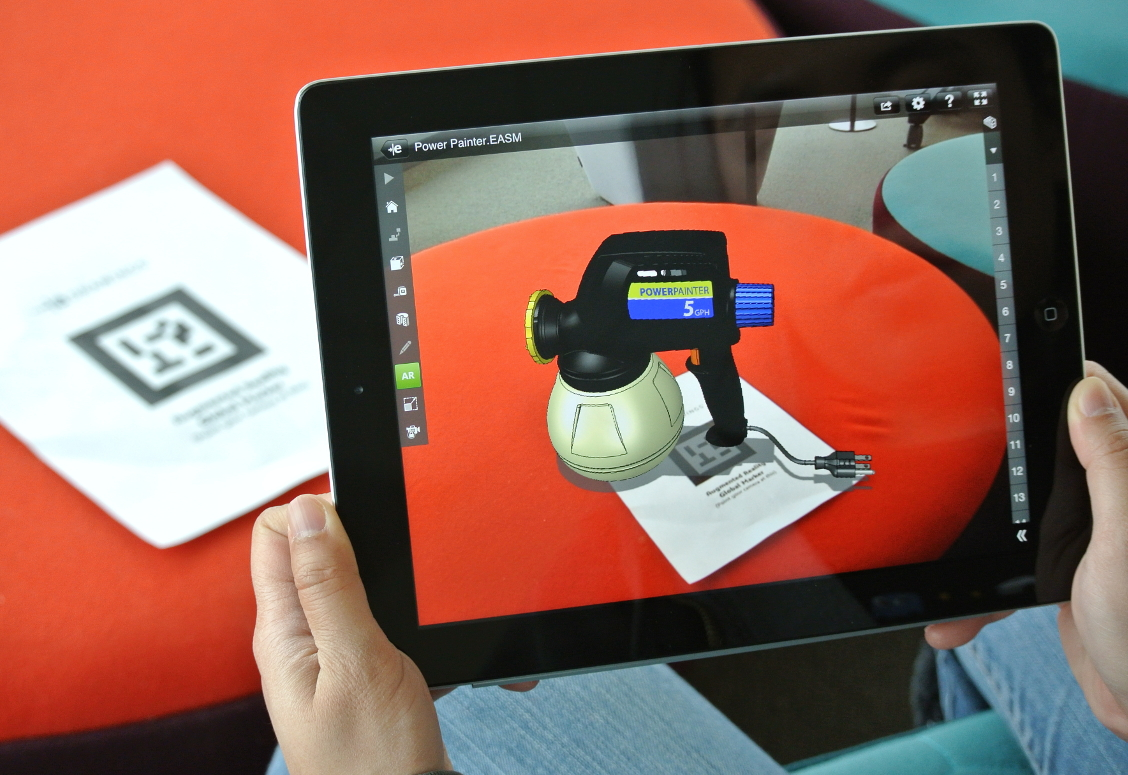
\includegraphics[scale=0.9]{pics/fiducialexample.jpg}
	\caption{Typical Augmented Reality application with fiducial markers}
	\label{fiducialexample}
\end{figure}

For applications like this to work, markers, usually perfect squares, are
created. This is so that the program detecting the markers is able to
take in information from the user about the markers' real world dimensions,
i.e. the length of the sides of the marker. From there the corner points 
of the marker are detected in the image. The realitive length of the sides 
then constructed from these corner points are worked out and
compared to the known truth. Performing these calculatiosn allow the 
program to work out the tilt of the marker, along with its 
distance from the camera and its rotation. These allow the 3D image to be 
rendered with the corresponding properties allowing rotation, tilt,
translation etc. of the 3D image when the marker is moved within 
the video feed.

\subsubsection{Markerless Augmented Reality}
Obviously, having a marker in the scene is not always desirable.
In my own opinion, having a marker in the scene makes the whole
experience less interesting. The reason for this being is that there is
a clear object in the output image that offers a  
separation between what is real and what isn't. Of course, there
are many situations where this does not matter, but if you could 
remove the marker, the scene becomes one step towards being mistaken
for a true reality.\\
\\
Markerless Augmented Reality is seeing a lot of research nowadays, if not
for the same reasons I just mentioned, another reason could be it may not 
be easy or even feasible to place a marker in the scene. 
To combat this, we must
look to other things to help us anchor our scene and graphics. This is done
through \textit{implicit markers}; things in the scene that arent defined
as markers but due to properties such as remaining more or less constant 
as it is viewed in the scene, it can be referred to judge the state of other
things in the scene. The more implicit markers used and detected, the more
likely the scene is to be understood by the program correctly as there is
now a higher amount of ground truth available.\\
\\
Take, for example, beauty company, Sephora's, augmented reality mirror.
This application just takes a video feed of someone's face and will allow
them to augment onto themselves, different kinds of make up! Obviously 
this wouldn't be a hit with their patrons if they had to place some 
fiducial markers on their face. First, it will obscure part of the face, 
which is the main thing
the user will be looking at, and it would also make the user feel a bit 
silly. \\
\\
As aforementioned, markers can be anything, inculding implicit markers,
preferably ones that are easily identified. For Sephora, these implict
markers will likely be the eyes, the mouth, possibly ears and jaw line.
The reason for this is that the eyes and mouth are the main areas to
apply makeup, in addition, ears and jaw stand out and the rough positions
of all other facial structures can be determined from them! It is quite
easy to begin identifying eyes and mthe mouth due to their shape, 
e.g. eyes will be circular, lips oval in shape. In addition, there will
be a large change in colour between skin and eye white and then eye white
and iris colour. As a result, when the program identifies such a point with 
these shapes and a sharp difference in the colour, it
is likely an eye and can be used as an anchoring point!\\
\\
However, using implicit markers leaves more room for possible error and
misdetection will lead to the application not working some of the
time. In the retail industry, this can cause loses in sales and revenue 
and can mean a lot to a company and their image. As a result, there
have been many investigations into making markerless Augmented Reality
better and better, this starts at the root, which is the Computer
Vision aspect of Augmented Reality. Computer Vision is a massive field, it is
mainly concerned with being able to segment and break
down an image into different objects and parts, then identifying which
parts are the ones important to track or to use.

\subsection{FINAL CHECK - Construction of Augmented Reality scenes}
Augmented Reality has two main parts to it; Computer Vision and Computer Graphics.
There may also be all sorts of other computer science topics melded in, for
example Machine Learning, Artificial Intelligence to name a couple. 
The pipeline in Figure \ref{fig:arpipeline} describes how a basic Augmented Reality 
application should be created.\\

\begin{figure} 
	
\includegraphics[scale=0.5]{pics/ARpipeline}
	\caption{Augmented Reality pipeline.}
	\label{fig:arpipeline}
\end{figure}

The middle stage, where the data from Computer Vision methods is processed. 
In this stage we can usually slot in Machine Learning or other kinds 
of data manipulation, before handing it over to be rendered by the Computer
Graphics part of the application. For the purposes of this project, I will not need,
nor do I intended, to stray from this basic pipeline where data processing in 
the middle will be minimal.

\subsection{FINAL CHECK - Computer Vision and Image Processing}
Computer Vision is a massive topic in the field of Computer Science. It
involves taking an image and performing various algorithms on it so that
the image can be better understood by the computer. For example,
passing in a simple photograph and having the computer output a box
around the recognised faces in the photograph. This is exactly the
functionality we see in most modern day smart phone cameras! Computer
vision is everywhere and is a widely studied area.\\
\\
Computer Vision is not limited to pictures, we can extend it to 
computer generated images and video. Anything we can see, we can pass to 
the computer to represent in a way it can understand and
store. The field also finds itself intertwined with other areas of
Computer Science due to its range of applicability and its plethora
of possible use cases. Some areas include Machine Learning, Robotics,
Medical surgery and Imaging, the list goes on.\\
\\
The topic of Computer Vision is so large that it can be split into
many subdisciplines. Some of these subdisciplines include
Image manipulation, Segmentation, 
Transformation, Filtering, Feature Extraction, Image Registration,
Tracking and more. Due to the sheer size of this field, within 
this master's thesis I will only 
introduce the main topics used in Augmented Reality: Feature 
Recognition and Extraction, along with Image Manipulation.

\subsection{FINAL CHECK - Image Manipulation/Processing}
Image Manipulation involves taking an image, be it a photograph or 
computer generated image, representing it in a way that is understood
by the computer and then performing actions on this representation.\\
\\
In Augmented Reality, Image Manipulation is typically used to help in
Feature Extraction and Recognition. In these areas, "important" features and
objects are identified to track. However, it is sometimes hard to fully
distinguish what should be identified. Image manipulation can offer methods
to alter the image in such a way that these features stand out more in terms
of computer representation. For example, an Image may be converted to 
black and white
(or the pixels in dark areas made darker and the bright areas brighter),
where the white areas are areas of interest and the black areas are places
which do not need to be considered. Other manipulation techniques will
involve looking at pixel colour values and gaining some understanding of
the picture based on the collectin data. With this data, the program can
perform different functions to change the picture.

\subsubsection{An Image in the computer}
A computer displays a picture with \textit{pixels}. A pixel is the
smallest unit of an image. A 2D array of pixels will make up an image.
The more pixels you can fit into an area, the better quality a picture
you can show on the screen.\\
\\
Pixels hold values which describe how they should appear to the user, this is
essentially the colour of a pixel. There are many \textit{colour spaces} that
an image can be represented in. What this means is that there are
various ways to represent the value of a pixel, the most common colour
space is the RGB model, where each pixel is given a Red, Green and Blue
colour value, which, when combined, will give the resultant colour of the
pixel. The ranges of these values are typicall 0 to 255. 
For example, \texttt{(0,0,255)} indicates a completely blue pixel. 
Figure \ref{fig:pixels} shows a few more examples. However, there are 
also different colours spaces, such as BGR (where B and R values are
switched), Grayscale which has one value per pixel (0-255), and Binary
colour space (pixels are either black or white).
An image is a 2D array of these pixels.

\begin{figure}
	\centering
	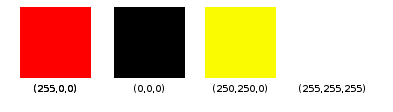
\includegraphics[scale=0.9]{pics/pixels.png}
	\caption{Pixel values and colours in RGB space.}
	\label{fig:pixels}
\end{figure}

\subsubsection{Image masks and operating on an Image}
To manipulate an image, the computer applies functions to images,
these functions typically iterate over each pixel in the provided image and
make changes to the image at the pixel level.\\
\\
Images can be aligned to each other (Image Registration), where pixels
will be matched to obtain an optimal alignment. Images can also
be rotated, translated, sheered etc. (Image Transformation) to, effectively,
shiftthe pixel values to different pixel locations. \\
\\
Using Image masks is one way of applying a function across an image.
Some uses of masks involve edge detection or blurring an image. In
Computer Vision literature, masks are also known as \textit{kernels},
or \textit{convolution matrices}. A mask is typically square in shape,
of an odd number in length. For example, a 3x3 mask or a 5x5 mask. 
Masks are then convoluted with the image, which itself is considered as
a matrix of values. Depending on the values in the mask and the convolution
algorithm, new pixels can be assigned the to middle pixel.\\
\\
To explain convolution, the peusdoalgorithm in Algorithm 
\ref{algo:gaussianblur}, and Algorithm \ref{algo:blur}, is used as an example.
The values of the kernel can be seen in Figure \ref{fig:gaussiankernel} .

\begin{figure}
	\centering
	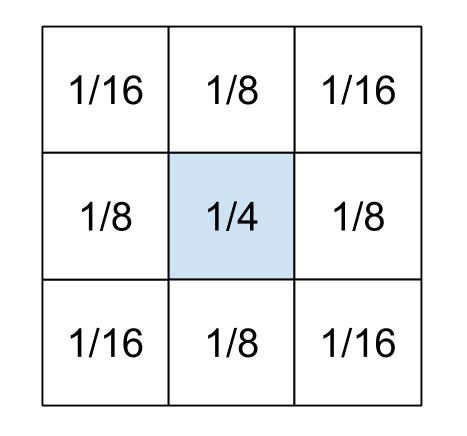
\includegraphics[scale=0.3]{pics/gaussiankernel.jpg}
	\caption{The Gaussian Kernel for blurring}
	\label{fig:gaussiankernel}
\end{figure}

\begin{algorithm}
\DontPrintSemicolon
$gMask$ is the 3x3 convolution matrix\;
Img is the image being blurred\;
blurredImg is the new blurred image with the same dimensions as Img\;
\Begin{
$newValue \longleftarrow 0$\;
	\For{pixel($i,j$) under $gMask(h,w$)}{
		newValue $\longleftarrow$ getPixelValue($Img,i,j)$ * $gMask(h,w)$\; 		
	}
	Set value of blurredImg pixel under the centre of $gMask$ to newValue\;
}
\caption{The Blurring Algorithm}
\label{algo:blur}
\end{algorithm}

\begin{algorithm}
\DontPrintSemicolon
$gMask$ is the 3x3 convolution matrix\;
Img is the image being blurred\;
blurredImg is the new blurred image with the same dimensions as Img\;
\Begin{
	\For{pixel($i,j$) $in$ Img}{
		align centre of $gMask$ with the first pixel in Img and blurredImg\;
		apply The Blurring Algorithm\;
	}
}
\caption{Convoluting a Gaussian kernel with an image to blur it.}
\label{algo:gaussianblur}
\end{algorithm}

\subsection{FINAL CHECK - Feature Recognition and Extraction}
Feature Recognition and Extraction is the other important Computer Vision
topic that will come into play in Augmented Reality. As Computer Vision can
be separated into many different topics and subtopics, from this point
onward, when I refer to Feature Recognition and Extraction, I also refer
to Object extraction (which is sometimes classed as a subtopic of
visual recognition).\\
\\
A feature in an image is a particular thing which
may be of importance to track. This could range from a shape, a corner point,
a certain pattern, a whole object etc. For Augmented Reality and 
the purposes of this project the areas of particular interest to us are 
Edge detection, Corner Detection and Object Extraction.\\
\\
In Augmented Reality applications that utilise a marker, Corner and 
Edge detection is used
to locate the marker in the scene.In markerless Augmented Reality, 
there is need to identify implicit markers, this is usually solved
by Object Extraction.  However, to begin Object Extraction, 
there is usually need to perform Edge detection first.

\subsubsection{Edge Detection}
% Detecting lines and edges of paper, for registration

\begin{center}
	In an image, an edge is a set of pixels that separates two disjoint
	regions.
\end{center}

A key part of Computer Vision is line and edge detection. Edge detection is
the very beginning of how we can start to identify different objects 
within an image. In addition, by stripping an image down to its comprising
edges, we greatly decrease the amount of information in the image whilst
preserving the important parts which we want to operate on. 
As a result, how edges are detected have a large contribution
to what we can do with certain images.\\  
\\
Edge detection tries to find the set of pixels that separate two 
disjoint areas of an image by analysing sets of neighbouring pixels and 
looking for discontinuities in intensity or texture. A variety of factors
can cause these (local) discontinuities:
\begin{enumerate}
	\item Object colour and texture. If the object has any change in colour or
		  texture, then where the change occurs, an edge will be detected.
	\item A change of surface normal. In the real world, we have 3D objects,
		  as a result, there will be a surface normal change when we consider,
		  say, the top face of a box against the side face. There is an edge
		  between the two and this is partly also due to the next factor...
	\item Illumination. A change of illumination or simply due to some
		  part of the object in question casting a shadow will cause some regions
		  of the image to be darker or lighter in intensity, even if said
		  regions are part of the same object. Edges will be detected in this
		  instance.
	\item Two objects. This a large part of why we even do edge detection, to
		  detect objects. If there are two objects, then, likely, there will be
		  a difference in colour and intensities of their constituent pixels.
		  However, this is not always the case and also as can be reasoned from
		  above, these regions may belong to the same multi-coloured object.
\end{enumerate}


We can distinguish edge detectors into two sets, the Laplacian (of 
Gaussain)-based detectors and the Gradient-based detectors.

\subsubsection{Gradient-based detectors}
Gradient edge detectors look for changes of gradient (first-order) of 
neighbouring pixels. Some common gradient-based detectors are Sobel,
Prewitt, Canny and Robert. Each of these detectors starts off with an image
and an x and y kernel. The kernels help determine the gradient change in the x
and y directions of the image, different kernels (size and values) are what
separate the different Gaussian-based detectors. For example, some kernels
may be 3X3 and others 5X5 or even 7X7. The size usually affects how
sensitive the operator is to an edge while values will determine how much
each pixel in the neighbourhood will contribute to the final outcome
of the operator for that pixel. The final gradient magnitude
for a given pixel is then the square root of the sum of the x and y
magnitudes for that pixel: 

\begin{equation}
	G = \sqrt{\Delta x^2 + \Delta y^2} 
\end{equation}

Users can then set a threshold value for which any pixel with a final
gradient that is above that threshold will be treated and marked as an edge,
the others will be discarded. Thresholding is the way in which we 
ultimately find edges and lines within an image, a good threshold value is
required to have good edge detection and can be image dependent as
the innate properties of images may be hidden due to other properties such
as colour or overexposure.

\subsubsection{Laplacian (of Gaussian)-based detectors}
Laplacian based detectors are similar to Gradient-based ones except that 
instead of taking the first derivative, they consider the second derivative.
Their goal is to look for zero-crossings, i.e. local maxima in 
gradient changes (i.e. looking for when gradient starts going negative). The
change of gradient sign, which occurs when second order derivative is 0,
indicates that the intensity of the observed pixels begins changing also. This
method can be coupled with a Gaussian kernel which serves to de-noise the
image by smoothing out the pixel intensities. 

\subsubsection{Corner Detection}
Edge detection is not always a good way to identify what is within a scene.
In the real world, there are many objects within the scene and they can
cause many edges to be detected with typical edge detectors. When trying
to understand a scene that has a lot going on, it is very difficult
to begin doing this with edges. Instead, it may be better to track certain
\textit{feature points}, which are discrete, rather than continuous features
such as edges. In addition, it can be much easier to identify an object by
these feature points rather than having to identify the relation of each
edge point to another. It greatly reduces the amount of information to be
stored and compared if done in this way. Another problem is that when
edges are detected, it is not always 100\% accurate. There can be gaps
and misdetections along with connectivity problems between sets of points
along an edge.\\
\\
Corners are an example of feature points. There are several corner detection
algorithms out there, the earliest of which comes from Hans Moravec. His
original detector wasn't intended as a corner detector, but rather a way
of identifying features to track to navigate a robot (the Stanford Cart).
However, the algorithm a few flaws and so was improved on by Chris Harris
and Mike Stephen's, making the Harris/Stephen's corner detector. Their 
paper \textit{A Combined Corner and Edge Detector}\cite{Harris88} 
highlights both of these corner detectors.\\
\\
\underline{Moravec's Corner Detector}\\
Moravec's corner detection algorithm works on the basis that you can,
very likely, identify a corner by considering a window of pixels and
examining them in turn as the window shifts. It is possible to do this
as there are three possible scenarios when considering a window of an image:
\begin{enumerate}
	\item On a solid area (Fig \ref{moravecsolid})
	\item On an edge (Fig \ref{moravecedge})
	\item On a corner point (Fig \ref{moraveccorner})
\end{enumerate}

These instances are illustrated in the pictures below in 
Figure \ref{moravecinstances}. The corresponding windows can be seen on the
original image in Figure \ref{moravec}.

\begin{figure}[h]
	\centering
	\begin{subfigure}[t]{.3\textwidth}
		\centering
		
\includegraphics[scale=1]{pics/moravec1.png}
		\caption{Solid window}
		\label{moravecsolid}
	\end{subfigure}
	\hfill
	\begin{subfigure}[t]{.3\textwidth}
		\centering
		
\includegraphics[scale=1]{pics/moravec2.png}
		\caption{Window over an edge}
		\label{moravecedge}
	\end{subfigure}
	\hfill
	\begin{subfigure}[t]{.3\textwidth}
		\centering
		
\includegraphics[scale=1]{pics/moravec3.png}
		\caption{Window over a corner}
		\label{moraveccorner}
	\end{subfigure}
	\caption{Window instances}
	\label{moravecinstances}
\end{figure}

\begin{figure}[h]
	\centering
	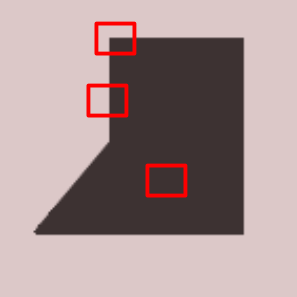
\includegraphics[scale=0.6]{pics/moravec.png}
	\caption{Sample image to detect edges on}
	\label{moravec}
\end{figure}

In order to obtain a measure of how likely the window is to be covering
an edge point, the window is advanced in various directions (typically
horizontal, both up diagonals and vertical) by a small 
amount and the image intensity measured. This is compared to the original
window intensity to help determine the nature of the window. In the end, 
a SSD (sum of squared differences) is used to obtain a measure of ``change".
If we call this measure $E$, the formula for computing $E$, the
change between a window and one of its neighbouring windows is:

\begin{equation}
	E(u,v) = \sum_{x,y} w(x,y)[Intensity(x+u,y+v)-Intensity(x,y)]^2
\end{equation}

Where the values of $u$ and $v$ are typically $\in (-1,0,1)$, i.e
$(1,0), (1,1), (0,1), (-1,1)$. The function $w$ just states that
this function applies for only those in the appointed window being 
considered. The function returns 1 if the pixel is in the window, 0 
otherwise.\\
\\ 
In the three scenarios listed above:
\begin{enumerate}
	\item If over a \textbf{solid} area of the image, a change in the
			window is likely to bring you over another solid area, so
			the change in intensity will be small.
	\item If over an \textbf{edge} in the image, a shift along the edge
			direction will cause a small change as you will be travelling
			along the edge. However, a shift perpendicular to the edge will
			likely bring you to a solid area, causing a large change in 
			intensity in this direction.
	\item If over a \textbf{corner} within the image, a shift in either 
			up, down, left or right will usually bring about a significant
			change in the intensity of the resulting windows. The SSD measure
			further intensifies this difference to give a large value for $E$.
\end{enumerate}

Thus, from these results, it is possible to set a threshold for which 
any resulting value of $E$, if it is above the threshold, can be considered
as a corner point to track. The corner strength of the window is then
taken to be the smallest SSD between the window and its neighbours.\\
\\
There are several things that could be identified as wrong with this 
algorithm, Moravec stated that the detector is not isotropic. In the
event there is an edge that is not in the direction of its neighbours,
the corner strength will be large
causing this type of edge point to be identified as a corner. Harris
and Stephens outline other reasons being:
The anisotropy comes from the discrete shifting of the windows every 45 
degrees. In addition, due to the binary nature of the windowing 
function, $w$, there can be noise generated in the image as each 
pixel within the window is given an equivalent weight in the SSD measure.
Finally, the detector responds to edges a lot as the corner strength
is determined by the lowest SSD, more on this point can be read from
their paper\cite{Harris88}.\\
\\
\underline{Harris/Stephens Detector}\\
The Harris/Stephen detector is a popular corner detector to use. It builds
on the weaknesses of the Moravec corner detector by offering solutions
to some of the problems in Moravec's detector.\\
\\
To counter the fact that Moravec's detector is affected by noise, Harris
and Stephens use a Guassian window function rather than a binary one,
with the the function being centred at the centre point of the window.\\
\\
To counter the anisotropy of Moravec's detector, instead of just a couple of 
shifts, all shifts are considered using a Taylor series expansion. First
order gradients are approximated such that the small shifts can be expressed
as the following equation, further explanation of this method is
in their paper\cite{Harris88}:

\begin{equation}
	E(u,v) = Au^2 + 2Cuv + Bv^2
\end{equation} 

The Harris/Stephens corner detector also utilises eigenanalysis in the
intensity change between windows depending on the direction of the window 
shift. Eigenvalues that are large typically depict an interest point
while if both eigenvalues are small, we are likely above a solid area,
a point we don't have to be concerned with. If both eigenvalues are large,
we have an area of interest, i.e. a corner. \\
\\
The Harris/Stephens detector is generally better than the Moravec 
detector as it works to fix its identified flaws, other attributes of
the detector are that it is rotation invariant (depending on eigenvalues 
means that since the shape is the same, the values will be equivalent). 
It is also somewhat invariant with transformations to the picture
intensities as gradients are used (Taylor expansion). Scaling the
image will affect the detector though, it is essentially the same
affect as making the window larger or smaller, scaling an image
could place an original non-corner point in such a position in the
window that it will be detected as a corner.

\subsubsection{Object Detection}
Object detection is a massive field and there are many 
different ways to identify an object within a scene. For 
example, gradients in an image can be used to identify 
parts of an object or which area of the image is likely 
to belong to the same object much like it is used in edge
detection to segment areas. Texture or intensity histograms 
store how many pixels of each object belong to a set of 
identified textures or intensities and histograms can 
be compared to see if we are looking at the same object. 
Plain template matching can be used to identify objects 
in a scene, for example cars or motorbikes, where the objects 
do not vary too much in shape, if the area the template 
is compared to has a good similarity, the object can be 
identified. \\
\\
Corner points, an example of identified features in a scene,
are a good start point for Object detection. By processing
images in sequence (in video), and being able to pull out
corners, if the object only undergoes rotation and translation,
the corner points can still be identified and an understanding
of where the object has moved, if at all, can be worked out.
However, there will likely be many corner points identified
in a scene. With fiducial markers, the reason why they are
mainly square in shape is to compare ratio of sides. When
corner points are identified, a quick calculation of the
length of sides can be calculated, sides opposite to
one another should have a ratio of around 1 even if 
the object undergoes rotation and translation. The question
then becomes what if there are several square objects within
the scene that aren't actually fiducial markers? That is
where template matching or intensity/histogram measures 
can be utilised. For example, there may be a set of fiducial
markers stored in a database. When a square has been detected,
then the object within the square can have a similarity
function run against it with the stored markers. If it 
comes into a specific similarity range, we can identify the
found object as the marker. Alternatively, the marker
is given a unique pattern that is able to be encoded into
a certain value based on the intensity of pixels within the
square. An example would be to divide the square into 5 
strips of 5 pixels, having 25 pixels in total. Each of
these can be black and white, thus there could be
$25^2$ different symbols such a square can represent 
(actually the resulting number of symbols will be much less
as the pictures will have to be unique, so one symbol
that is a rotation of another will not work though the 
principal is the same, being able to work out the 
represented value which uniquely identifies the marker
from other markers along with plain squares).\\
\\

\subsection{FINAL CHECK - Contours and Ordnance Survey Maps}
Ordnance Survey(OS) are an agency for Great Britain that specialise in
making maps. The agency was formed around 1791 and has
been producing maps for Britain since. Ordnance Maps are, of course, 2D and
are produced on paper, long before maps could be accessed online, such
as GoogleMaps. OS maps were a staple to any adventurer travelling Britain's
landscapes. Below, in Figure \ref{OSmap}, is a segment of a typical OS Map.

\begin{figure}[!h]
	\centering
	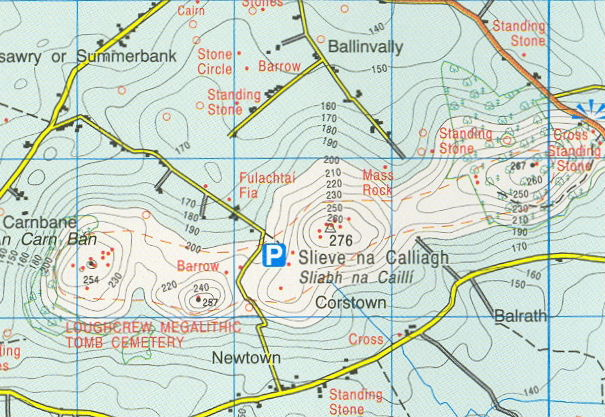
\includegraphics[scale=0.7]{pics/OSmap.png}
	\caption{OS Map snippet}
	\label{OSmap}
\end{figure}

The curved, grey, lines which have numbers on them are contour lines. These contour
lines dictate the height of the land (above sea level) at that point. All points
along the contour are of the stated height. The OS map standard is 
that every next contour is a difference of 10m from the last. 
In addition, every 50m has a thicker contour. As a result, OS maps 
accurately depict hills, mountains
and elevated land. The contours used for landscape maps in this project are 
heavily based off of OS map contours. A possible, advanced use for this project
is to turn OS maps into 3D representations and port the application to
a mobile device. This would allow travellers who are
out in the field with no internet reception for their favourite map application to
simply hold view a 3D version of the OS map they should have taken on their journey.
Of course, there are many other factors invovled, such as extracting other lines
which may represent road or river and determining what is actually a land contour, 
this idea is one to keep in mind, however.\\
\\
Another trait to notice about contour lines is that their proximity to each other
also indicates how steep the slope of the area is. If contours are close, such as
near the peak of the Slieve	na Callaigh in Figure \ref{OSmap}, then the land is 
steep. If you compare this to somewhere such as near Ballinvally, the contours 
are much further apart, indicating a flatter, less steeply increasing/decreasing 
slope. 

\subsection{~DO~ Computer Graphics and Rendering AR Scenes}
Computer Graphics is also a very large field in Computer Science. It is
concerned with producing pictures or video with which objects in the
medium have been created by the computer. With relation to Augmented
Reality scenes, graphics is concerned with generating the frame of
a 3D model. Onto this, there may or may not be textures, colours and
illumination applied. The main problem comes with aligning the object
with the scene in real life. This is because each of the components
of Augmented Reality is rendered in its own coordinate space.\\
\\
When working with an Augmented Reality application, the following
coordinate spaces have to be aligned:
\begin{itemize}
	\item Real World coordinates
	\item Camera Coordinates
	\item Model Coordinates
\end{itemize}

In addition, there also has to be a specification of what the 
user should be able to see, which is described through a 
\textit{Projection Matrix}.

\subsubsection{Real World Coordinates}
Real world coordinates are where objects are situated in the real world.
There is some defined origin and objects have


\subsection{FINAL CHECK - Existing Augmented Reality Projects}
Within this section, I outline a couple of existing Augmented Reality 
applications which perform similar, but not the same functions as 
what my project is proposing to solve.

\subsubsection{LandscapAugmented Reality}
\label{LandscapAugmented Reality}
Looking into the Augmented reality scene and potential similar
applications brought me across the mobile application \textit{LandscapAugmented Reality},
made by Stapps. The premise of the application is that it is aimed at
graphic/landscape designers and turns drawn contour lines into an augmented
reality environment you can view through your phone screen. \\
\\
The application imposes several restrictions upon the user, however. The user
must use a thick black pen for the app to successfully identify contours. 
In addition, the user must make sure that every contour is properly connected
and closed. Already, this limits some things that the user is able to do.
Users also have to take the time to be precise with their handywork and also 
must make sure they have the 
correct equipment to start creating their work. In addition, the application
requires the user to place white paper over a dark background/table otherwise
the scene may not be recognised. Even if the paper is on a dark table, it 
does not guarantee the paper is identified, this may be due to illumination
differences of the whole paper not being fully captured, as in 
Figure \ref{fig:landscapeAugmented RealityNoPaper1} and \ref{fig:landscapeAugmented RealityNoPaper2}.This 
is likely because the application uses 
the paper edges/corners as anchor points upon which they can align the 
augmented scene and use registration to align the output. In addition, it
is possible for the paper to be "too far" away from the camera, when I
myself tested this, it caused a good several minutes of frustration trying
to align the phone camera and the paper such that the application could 
function seen in Figure \ref{fig:landscapeAugmented RealityNoTooFar}.\\
\\ 
Finally when all this is done, the user must press the "Scan" button
which can cause them to lose their hard-sought alignment! An original
topdown view is generated, see Figure \ref{fig:landscapeAugmented Realitytopdown}, on
the first scan. After, the user can choose a free camera mode where they 
can move the camera around to view the scene in 3D, 
Figure \ref{fig:landscapeAugmented Realityangled}, though the ability to steadily
keep this image on the screen is lackluster in some scenarios.  \\

\begin{figure}[!ht]
	\centering
	\begin{subfigure}[t]{.4\textwidth}
		\centering
		
\includegraphics[scale=0.3]{pics/landscapeARNoPaper.png}
		\caption{The user must align their paper properly}
		\label{fig:landscapeAugmented RealityNoPaper1}
	\end{subfigure}
	\hfill
	\begin{subfigure}[t]{.4\textwidth}
		\centering
		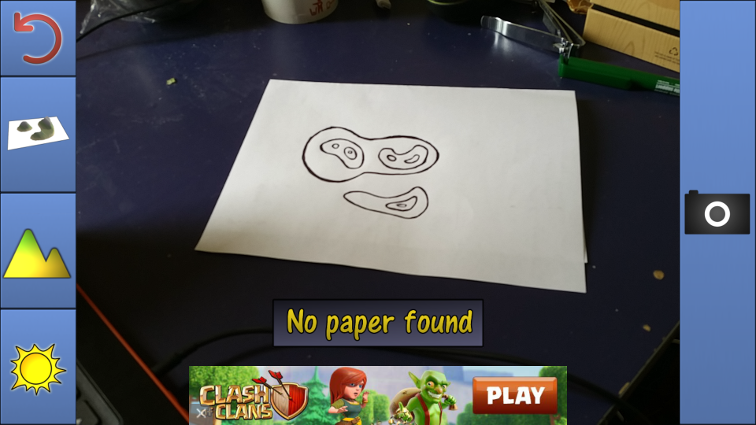
\includegraphics[scale=0.3]{pics/landscapeARNoPaper2.png}
		\caption{The user must align their paper properly}
		\label{fig:landscapeAugmented RealityNoPaper2}
	\end{subfigure}
	
	
	\begin{subfigure}[t]{.4\textwidth}
		\centering
		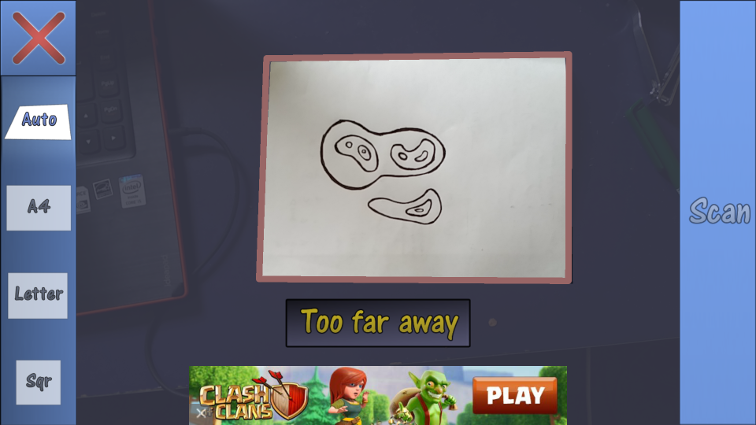
\includegraphics[scale=0.3]{pics/landscapeARTooFar.png}
		\caption{The range of detection is limited.}
		\label{fig:landscapeAugmented RealityNoTooFar}
	\end{subfigure}

	
	\begin{subfigure}[t]{.4\textwidth}
		\centering
		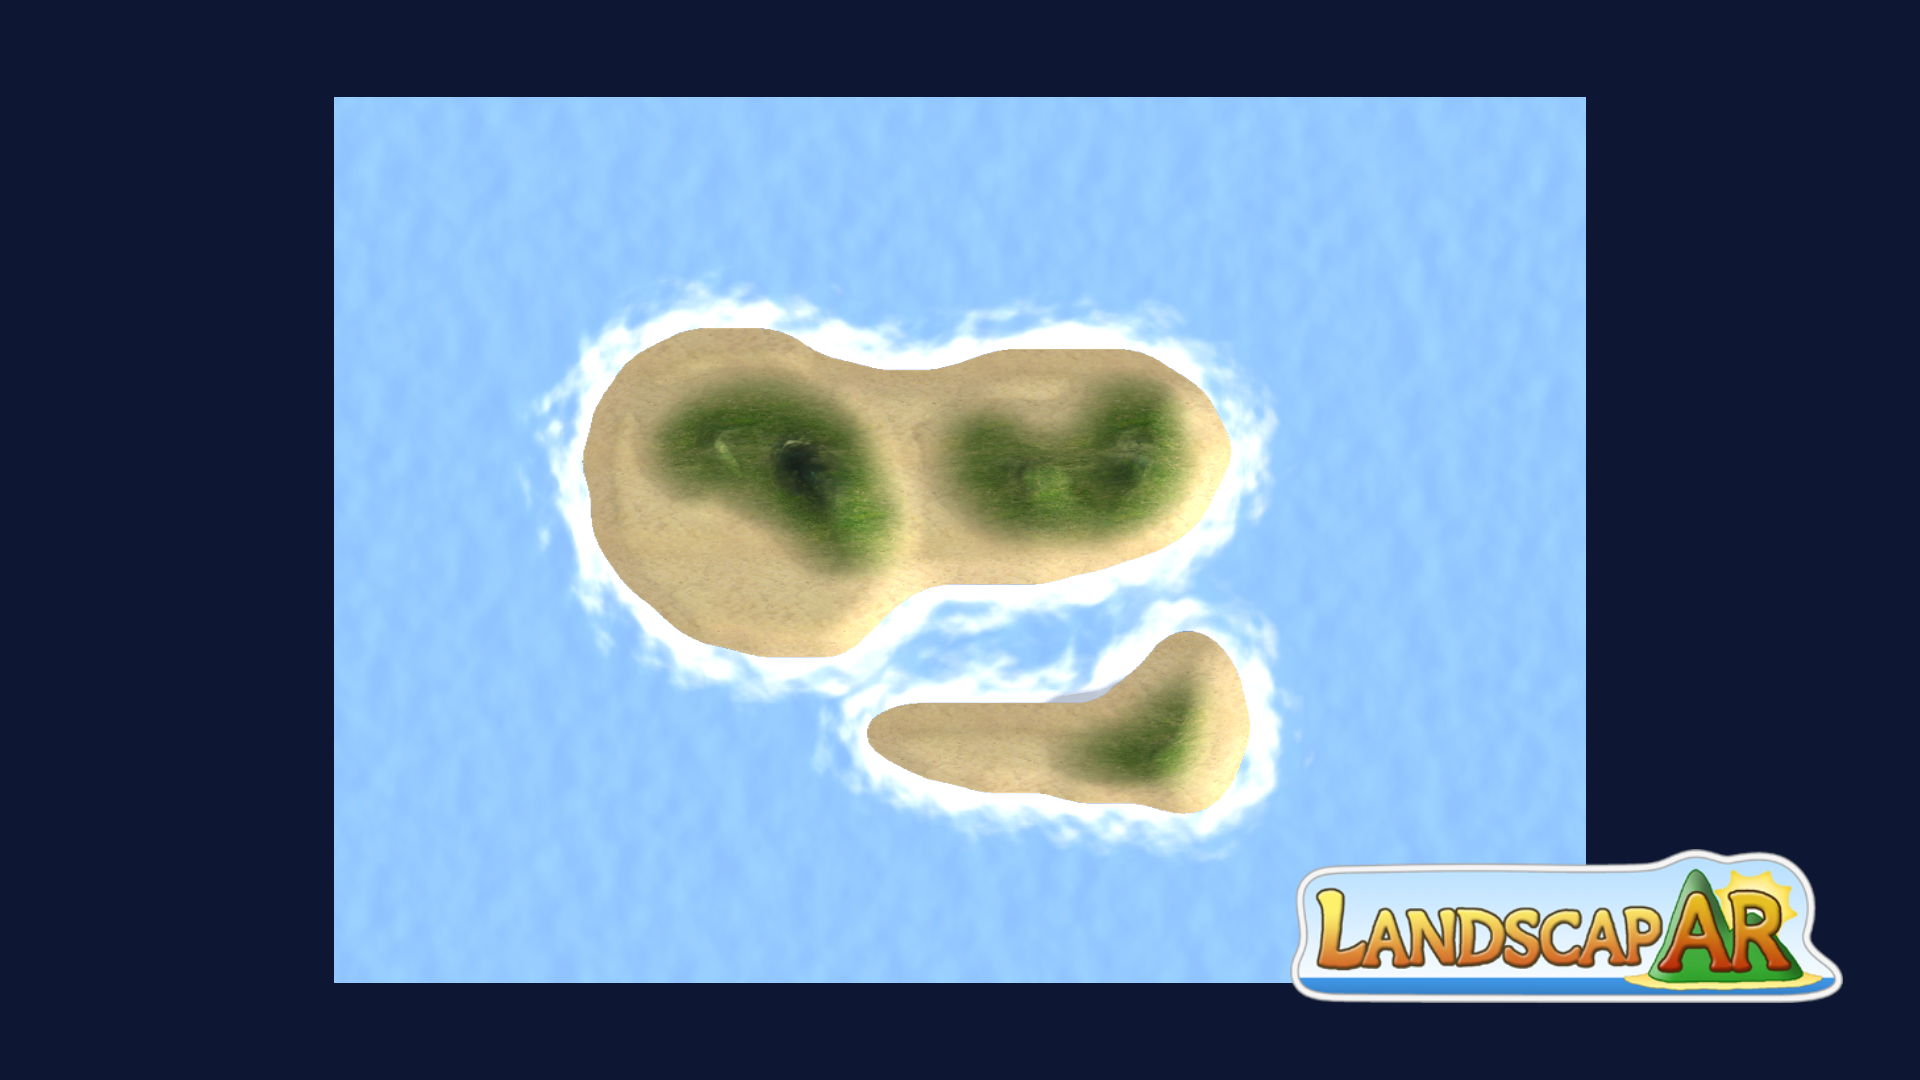
\includegraphics[scale=0.3]{pics/landscapeARtopdown.png}
		\caption{Output from a simple scan produces a top down image}
		\label{fig:landscapeAugmented Realitytopdown}
	\end{subfigure}
	\hfill
	\begin{subfigure}[t]{.4\textwidth}
		\centering
		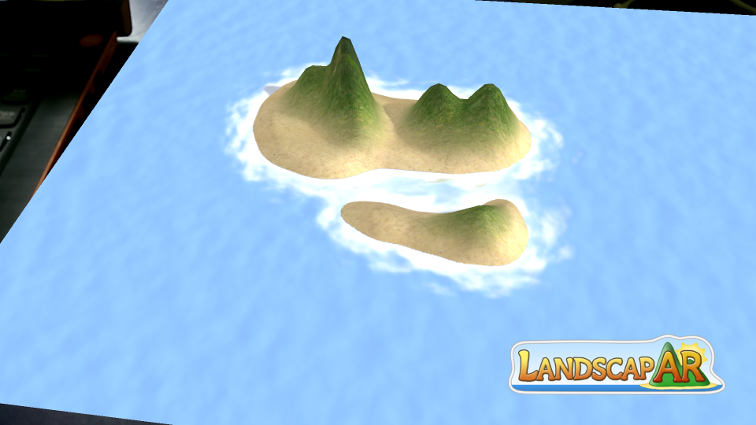
\includegraphics[scale=0.3]{pics/landscapeARangled.png}
		\caption{After scanning it is possible to move the camera}
		\label{fig:landscapeAugmented Realityangled}
	\end{subfigure}
	\caption{Testing LandscapAR}
	\label{landscapAugmented Reality}
\end{figure}

There are several ways that this application can be improved. For example,
currently the user has to draw their contours on a piece of paper and then
scan paper using their mobile device. The scanning process itself is quite 
cumbersome as trying to get the system to detect paper can be hit and miss.
The scan analyses the image and overlays a 3D scene onto it quite well, however
the downfall with this is that to make updates to the scene, ou use has to
re-scan the image after addition, adding more cumbersome steps. For users
who want to make several small changes here and there, this will consume a lot
of time and effort on their part.

\subsubsection{The Augmented Reality Sandbox}
The University of California, Davis along with the Lawrance Hall of Science 
and ECHO Lake Aquarium and Science centre contribute to a project called the
Augmented Reality Sandbox\cite{Reed14}. The project allows users to turn a 
typical sandbox
into a creative landscape environment, much akin the goal of this project.
The system uses a Microsoft Kinect 3D camera along with a projector to 
perform its magic. Both are positioned above the sandbox and the depth 
camera on the Kinect
will measure the local relative depths of the sand in the sandbox. If the
user has created mounds on the sandbox the peaks of the mounds
will be closer to the camera, these will be converted into mountains/hills. 
Areas lower than a certain threshold 
depth will be converted into water. The input from the 3D camera will pass 
the data to a computer and project subsequent land/water colours onto the
corresponding areas of the sandbox.\\
\\
The Augmented Reality Sandbox also has a variety of other functionalities, such
as creating rain over the Augmented environment by hovering a hand over the 
area you wish there to be rainfall. The whole project aims to teach people, 
particularly children, about landscapes, watersheds and catchment areas 
that you can physically change, interact with, and get real-time response 
from. The project has gained quite a bit of interest, with alternate 
versions being built by others and is something that helped in the 
motivation for this project. The sandbox can be seen in Figure \ref{arsandbox}. \\

\begin{figure}[!h]
	\centering
	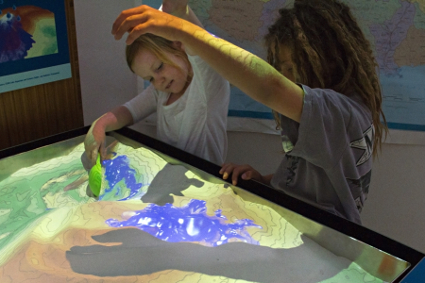
\includegraphics[scale=0.8]{pics/sandbox.jpg}
	\caption{Children learn about watersheds with Augmented Reality.}
	\label{arsandbox}
\end{figure}

The Augmented Reality Sandbox is a great tool for creativity, however it is very hard to set up
on a small, personal scale. Institutions and education centres can easily set
up and manage such a project but the cost and maintenance is hard for an
individual. In addition, the purpose is very limited and geared towards those
of the younger generation to learn simple concepts of geography. In this project,
I will be using the ideas the Augmented Reality Sandbox has put forward to offer an
improved, alternate version which is geared towards a much larger audience, with
less of a specific goal and more of an environment for creativity with less
requirement for special equipment like your own sandbox.

\section{FINAL CHECK - Hardware Investigation}
\subsection{Microsoft Kinect V2}
\subsubsection{Background \& History}
The Microsoft Kinect(V1) was originally released as an extra piece of hardware
for Microsoft's Xbox360 in 2010. The Kinect for Windows (V2) was released
in 2012 and offered a range of improved functionality from its ancestor, the
V1. Since its introduction into the market, the Kinect has received a lot of
attention from developers and it has seen many applications put forward for 
it. Many large companies have caught onto its capabilities and work 
alongside Microsoft and the Kinect to offer new experiences with the device.\\ 
\\
The Kinect V2 offers users the ability to track their
whole body with reasonable accuracy. In addition, the V2 can track up to 6 individuals
at one time with 25 body joints able to be placed onto the captured images.
This opens up a whole new range of applications
that the Kinect can be used for and this is apparent in the amount of interest in the
Kinect, along with the amount of published papers and success stories of 
its different use cases.
Some of the possible fields this device can be used include 
Augmented Reality, Entertainment and Games, Retail, Education and much more.\\
\\ 
"Evaluation of the Spatial Resolution Accuracy of the Face 
tracking system for Kinect For Windows V1 and V2" \cite{AmonFuhrmann14}
explores in more detail the increase in performance and capability
of the V2 and shows that it beats V1 in every aspect. 

\subsubsection{How it works} 
The V2 allows us to take infrared images along with 1080p colour images. It 
also has depth sensors to produce depth images. Inside the V2 are 3 infrared
emitters along with a colour camera, an infrared camera and some microphones.
These internal components can be seen in Figure \ref{kinectinternal}. The
microphones are along the bottom.
\begin{center}
	\begin{figure}[H]
		\begin{center}
			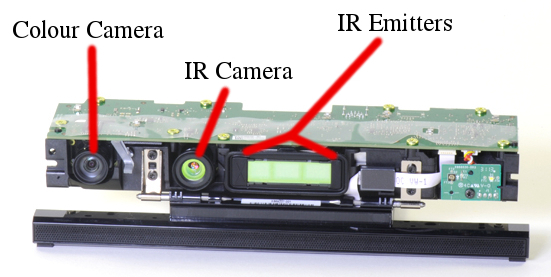
\includegraphics[scale=0.5]{pics/kinectinternal}
				\caption{Inside the Kinect V2 for Windows}
				\label{kinectinternal}
		\end{center}
	\end{figure}
\end{center}

The Kinect V2 differs from the V1 majorly in the way it produces depth maps.
V1 uses structured light while the V2 utilises Time-Of-Flight. Time-of-Flight
involves emitting many short bursts of infrared light (strobing it) and then
collecting it back through its camera. 
The technique involves splitting a pixel in half and collecting infrared light
on the pixel. However, each half is switche on at different times, 
while one half is on, the other is off and depending on the ratio of
how much light is collected by each half (ratio since it accounts 
for light absorption by objects in the scene),
the relative depth of objects can be inferred. \\
\\
The V2 also accounts for over exposure and saturation of pixels. This scenario
occurs when there are alternative sources of infrared light, i.e. in an outdoor
environment! The V2 can reset pixel values in the middle of an exposure, also
explained in Daniel Lau's blog mentioned above. This then
allows it to be used outside whereas the V1 wouldn't account for this and cause
all kinds of strange behaviour; this of course means that the scope for using
the V2 and its applications is significantly larger than it ancestor.
\\ \\
\subsubsection{My investigations} 
I investigated the Kinect for Windows first hand. In figure \ref{KinectDepth} 
you can see an example of the depth sensing capability of V2. On the right,
circled in blue, is myself. I sat around 40cm away from the camera. As I highlight 
in the limitations section below, this is reported as the minimum distance 
performance can be guaranteed by the V2. My friend, Juto Yu, is circled in 
yellow, he stays slightly outside the view of the camera, giving me a rough 
indication on how wide the capture region is. The green circled object is a 
pillar in the central library of Imperial College, it is definitely more than 
3m away from the V2 which is reported as the range before objects become 
"too far". Whether its detection is because the device can actually 
handle larger capure depths or due to the pillar being white and thus 
more reflective will need to be further looked into.
\begin{center}
	\begin{figure}[H]
		\begin{center}
			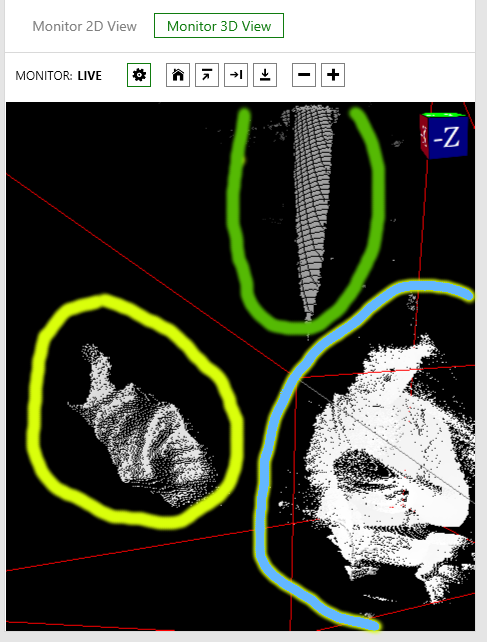
\includegraphics[scale=0.5]{pics/KinectDepth}
				\caption{Depth image from Kinect V2}
				\label{KinectDepth}
		\end{center}
	\end{figure}
\end{center}

I also looked into the colour camera's performance. The camera has a 1080p HD
video taking capability and is of a good quality. In addition, as seen in 
figure \ref{KinectColour}. The body tracking is pretty good and can make rather
accurate implications of people's limbs even when they are sitting down and are
obscured as shown. I was sitting at a desk but the V2 could make some guesses
as to where my legs would be. It is also clear that multiple tracking can be done
in real time at a speed that is responsive.
\begin{center}
	\begin{figure}[H]
		\begin{center}
			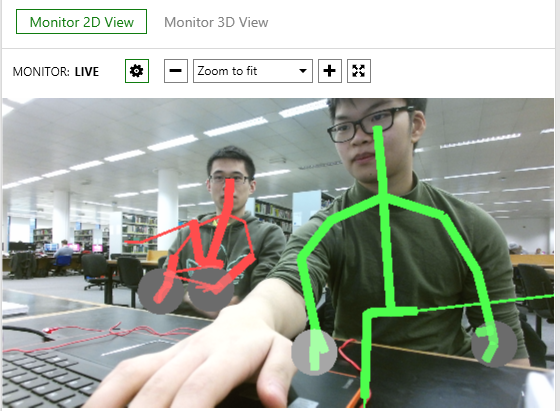
\includegraphics[scale=0.5]{pics/KinectColor}
				\caption{Colour Camera (with body tracking)}
				\label{KinectColour}
		\end{center}
	\end{figure}
\end{center}

The V2 is definitely a great alternative to some of the more expensive depth 
sensors on the market. As highlighted in the paper
"Low-cost commodity depth sensor comparison and accuracy analysis" by
Timo Breuer, Christoph Bodensteiner, Michael Arens. Some of the other sensors
that out perform it are upwards of £3000 while the V2 costs just around £150.
This means that it will be accessible to a much larger audience, something
definitely needed if an Augmented Reality game is to be successful.\\ 
\\
\subsubsection{Limitations and pitfalls}
The cameras of the V2 have a set range of values that it works well within.
This is reported by Microsoft to be from 0.4m to 3m
Anywhere beyond that seems to be too
far to determine the depth of objects. There is also a notion of being too near
to the device to! If we are working with the device, say, next to our laptop or
in a space nearby, there may be complications with how the sensor performs, 
anything closer than 0.4m produces unknown behaviour with the depth sensor.\\ 
\\
A pitfall I expect to encounter is when developing with the Kinect SDK. I have
experience in C++ which is one of the languages that can be used to write Kinect 
applications. However, it seems a lot of the colour camera tutorials are written
in C\# which will could cause problems for me if I had to pick up the language 
or translate it into the C++ equivalents. However, this should only be a small
pitfall and cause minor hindrance to the progression of the project.

\newpage

\section{Implementation}
\label{chapter:implementation}
In this section I outline the main steps I took in
the creation of this project. I will highlight some of the steps that I 
took to overcome some implementation problems. These will also be 
assessed later in the report in Section \ref{chapter:evaluation}.

\subsection{FINAL CHECK - Assumptions and Restrictions of the User}
\label{sec:assumptions}
This project started extremely broadly. I had many ideas and aspirations on
what the final product could do. However, I quickly realised that most
of these ambitions were unattainable in the time frame, at my level
of expertise, and with resources available to me. In light of this, 
some restrictions had to be imposed, implicitly, on the 
user when they use the program. Behaviour of the program outside of these
restrictions is currently undefined. This is not to say the program will not
work if these restrictions are not met but rather that the program has not been 
tested enough nor fine-tuned outside of the restrictions. 
In addition, I have designed my
program with a set of assumptions in mind that simplify the problem.
This project contains many topics within Computer Vision, 
Augmented Reality and Human-Computer
Interaction. If broken down and investigated in depth, some of these
could be whole research topics in themselves. The problem has thus been
reduced to one of less difficulty but which still achieves the original
goal. In this section, these restrictions and assumptions are listed. 

\subsubsection{Restrictions}
\begin{itemize}
    \item The ArUco marker is visible in the Camera
    \item The contour colour must be noticeable on the surface colour
    \item The user must have a fixed camera
    \item The angle of the camera to the lanscape map can't be too small
   	\item User must calibrate their camera themselves
   	\item The camera must \textbf{only} point at the landscape map and the
   			surface it lies on.        
\end{itemize}

In the ideal case, this project would have absolutely no restrictions 
on the user. To have otherwise means that creativity is constrained
to within the realms where these restrictions hold. As 
aformentioned, in this project, the goal of having absolutely no restrictions 
became infeasible. \\
\\
The subject of markerless Augmented Reality 
is being researched quite a bit now, however, current methods are rather 
cumbersome due to the real time requirement of Augmented Reality. Finding
and tracking an implicit object is quite difficult. As
a result, the user must have a marker on the surface they are drawing their
landscape map. \\
\\
In addition, if it is hard for humans to see the contour
lines, it is even more difficult for computers. With this in mind, 
the pen colour must
be of an adequately different shade to that of the surface it is drawing on.\\
\\
The user must also be able to calibrate their camera and make sure it
is fixed in the scene such that it can see the landscape map. The camera should
not be at too large of an angle to the surface otherwise 
the picture becomes way to difficult to understand and the contours hard
to recover.

\subsubsection{Assumptions}
\begin{itemize}
    \item The user draws perfect connected contours or near 
    	  perfect contours
    \item Light in the environment is stable and is not
    	  changing drastically over short time periods
    \item The user only draws with the intent of shapes being contours
    \item The user draws reasonably sized landscape maps and contours
    \item The user doesn't draw an extremely deep tree of nested contours
    \item The user typically starts the program with a landscape map drawn
    	  out already, as opposed to starting to draw only once the paper
    	  has been placed under the camera. The user then makes small 
    	  incremental changes to the landscape map, rather than complete 
    	  redraws.
\end{itemize}

I believe the above assumptions I have developed this project with
are reasonable quite reasonable.
Firstly, it would be very demanding of any Computer Vision program 
if a user drew an incoherent landscape map and hope for the program 
to understand it. Such a scenario requires a deep understanding of the scene,
the user's intentions etc. and may be possible to solve by machine learning
but even that is a stretch. \\
\\Secondly, it will be unlikely a user will be drawing the landscape map 
in an environment with rapidly changing light. If the user draws other 
shapes such as triangles, squares, etc., they will be interpreted as 
contours as this program only accommodates contours. \\
\\
It is also reasonable to assume that the user will not draw a 
miniscule landscape map as it becomes hard for both themselves and the camera
to understand what the scene is depicting.
The case of a large map is fine as the restriction of seeing the ArUco 
marker keeps the scale within reason, so long as the ArUco marker is not,
itself, miniscule to the point of being unrecognisable. \\
\\
We do not want a deep
tree due to the amount of contour level-traversal in the program. This
should only become a problem if the user begins at the very edges of the paper
and draws containing contours just one or two millimetres apart all the
way until they fill the paper, which is a rather uninteresting landscape map
anyway.

\subsection{FINAL CHECK - Computer Vision and Image Processing}
A key part of this project is the Computer Vision aspect. The field of
Computer Vision involves the understanding of data from images and pictures.
"Understanding" is a broad term that encompasses many ways of manipulating or
processing images in order to extract features or points of interest that
can be then used by the computer. \\
\\
To begin the project I looked into possible edge detection algorithms as 
this would allow me to start identifying drawn contours on a sheet of paper.

\subsubsection{Canny Edge Detector}
\label{sec:Canny}
% Detecting Contours for landscaping
There have been numerous methods of detecting edges put forward,
some Gradient-based and Laplacian based edge detection methods are 
outlined in 
\textit{A Comparison of various Edge Detection Techniques used in Image Processing}
\cite{Shriv12}. However, the most popular edge detector out there is the
Canny Edge detector, put forward by John Canny in his paper
\textit{A Computational Appraoch to Edge Detection}\cite{Canny86}. The paper
dicusses a mathematical approach to edge and ridge detection which is then
analysed in Ding and Goshtasby's paper, 
\textit{On the Canny Edge Detector}\cite{Ding00}. Rashmi's paper,
\textit{Algorithm and Technique on various Edge Detection: A Survey}
\cite{Rashmi13} compares various edge detection algorithms and finds that 
the Canny edge detector comes out on top, with Maini's paper 
\textit{Study and Comparison of Various Image Edge Detection Techniques} 
\cite{Maini} supporting the notion.\\
\\
The Canny Edge detector falls within the Gaussian-based Edge detectors and
can be described algorithmically below:
\begin{itemize}
	\item Apply a Gaussian filter over the image to remove noise by smoothing
	\item Take the gradient of the image pixels over each direction, just as
		  would be done in a normal Gaussian-based detector.
	\item Apply non-maximum suppression 
		  such that only local maxima are marked as edges (the pixel 
		  has a greater gradient magnitude than all
		  of its neighbours) resulting in a thin edge. The thinning of found
		  edges is to remove some effects of the blur. After this, perform
		  double thresholding, those higher than a threshold are "strong" edges
		  and those underneath are considered "weak" edges.
	\item Another round of removing edges is applied by using hysteresis.
		  This involves identifying "strong" edges,and then removing 
		  all edges that are not connected directly to these strong edges.
\end{itemize}

The steps are more fully explained in the paper by unnamed author 09gr820, 
\textit{Canny Edge Detection}\cite{09gr820}.

\subsubsection{Open and Closed contours}
We understand a closed contour to be a loop. By this we mean that if we had
to draw a closed contour, we begin at a point on a piece of paper and end at that
point, either by not removing our pen from the page or, if done so, will resume
at the same point to finish the contour. The existence of white space between
points on a contour mean that the contour is open and not closed. Examples
of open and closed contours can be seen in Figure \ref{fig:closedcontours} and 
Figure \ref{fig:opencontours}.
\\

\begin{figure}[H]
	\centering
	\begin{subfigure}[t]{.3\textwidth}
		\centering
		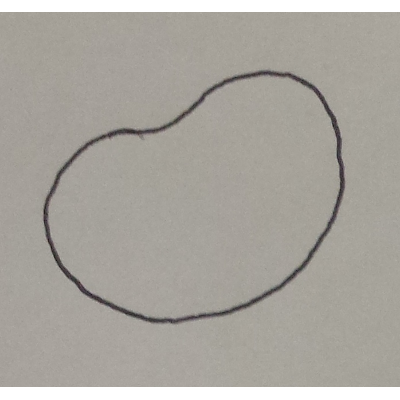
\includegraphics[scale=0.3]{pics/closedloop1.png}
		\caption{Contour is fully closed, no gaps}
	\end{subfigure}
	\hfill
	\begin{subfigure}[t]{.3\textwidth}
		\centering
		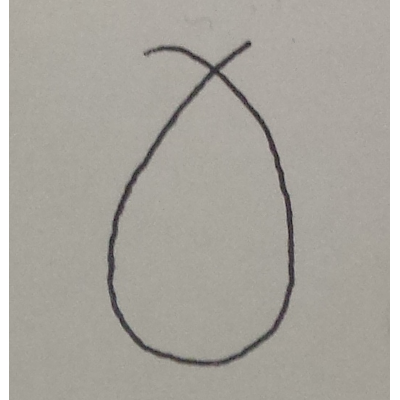
\includegraphics[scale=0.3]{pics/closedloop2.png}
		\caption{Contour is closed, but with artefacts on the ends}
	\end{subfigure}
	\hfill
	\begin{subfigure}[t]{.3\textwidth}
		\centering
		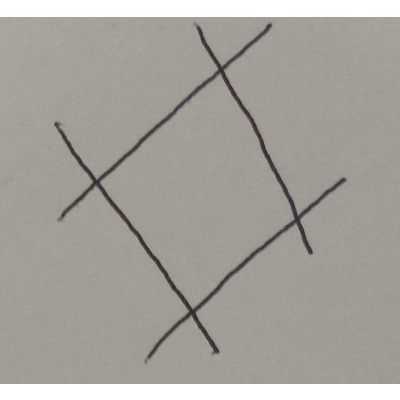
\includegraphics[scale=0.3]{pics/closedloop3.png}
		\caption{This is also a closed contour}
	\end{subfigure}
	\caption{Examples of \textbf{closed} contours}
	\label{fig:closedcontours}
\end{figure}

\begin{figure}[H]
	\centering
	\begin{subfigure}[t]{.3\textwidth}
		\centering
		
\includegraphics[scale=0.3]{pics/openloop1.png}
		\caption{A line/edge counts as an open contour}
	\end{subfigure}
	\hfill
	\begin{subfigure}[t]{.3\textwidth}
		\centering
		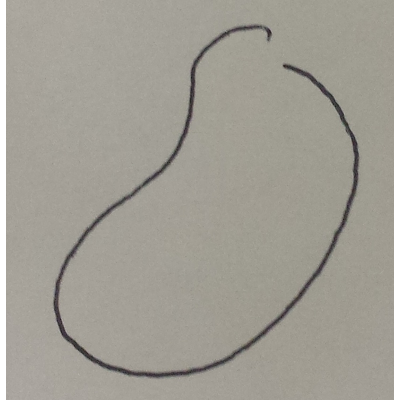
\includegraphics[scale=0.3]{pics/openloop2.png}
		\caption{Contour open as beginning doesn't connect to end}
	\end{subfigure}
	\hfill
	\begin{subfigure}[t]{.3\textwidth}
		\centering
		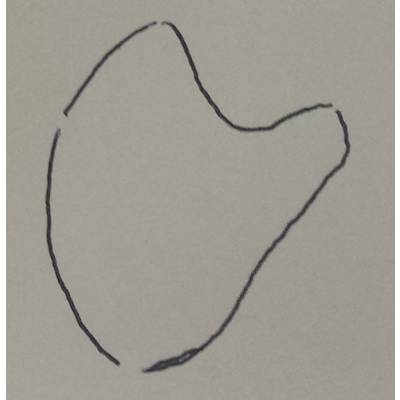
\includegraphics[scale=0.3]{pics/openloop3.png}
		\caption{This contour is open with several gaps}
	\end{subfigure}
	\caption{Examples of \textbf{open} contours}
	\label{fig:opencontours}
\end{figure}

For feature detection, and especially within this project, we look for 
\textit{closed} contours, they provide us with the most information. An open
contour may be related to some kind of feature point but if it is not closed,
it is essentially useless. We want closed contours so that any
contours that are drawn within them can then lend themselves to a natural
hierarchy/ordering, this will let the program which areas of an image
should be represented higher than others in terms of elevation. 
In the context of this project, contours contained within closed contours
will represent areas that are of higher elevation than the area contained between
itself and the outer contour. When contours are not closed, it becomes harder
for us to identify this hierarchy and ordering within the image. This
would result in a lot more difficult computation to be done to achieve
our goal of generating a corresponding landscape. Indeed, this is the problem of
many similar projects.

\subsubsection{Mathematical Morphology}
One technique used within this project 
to help close contours/loops in Computer Vision is \textit{Closing}.
To understand \textit{Closing}, we must first introduce the ideas of 
Mathematical Morphology (MM). MM is a method of manipulating geometric objects
and structures, typically used on images but can also be applied to other things
such as graphs. Within MM, there are four basic operators, but for the purpose
of this project, I shall only go into detail about the first three as 
the fourth is just an inversion of the third:

\begin{itemize}
	\item Erosion	
	\item Dilation
	\item Closing (Dilation followed by Erosion)
	\item Opening (Erosion followed by Dilation)
\end{itemize}

The operators were originally defined for binary images and so shall be 
described below in that sense, however, the functionality has been extended
to include grayscale images as well, which is very useful when dealing with
photographed images or video feed as will be done within this project.
\\
For these operators, let us assume there is a binary image, with pixels 
holding values of either 0 or 1. In correspondence to a typical colour image,
1 indicates white, a brighter area, of the image and 0 corresponds to a
black pixel, a darker area. In the erosion and dilation operators,
we have a binary image as the input. 
We also have a corresponding kernel which we will convolve
with the image. This kernel, sometimes referred to as a structuring element,
usually takes the shape of a circle, a 3x3 square or a cross. To achieve
different results from these operators, the kernels can be changed, for example
to a 10x10 square which will cause a more drastic shrink or growth of bright 
areas. For the purpose of explanation, I will assume use of a 3x3 kernel.

\subsubsection{Erosion}
\begin{center}
Erosion causes bright areas of images to shrink.
\end{center}

Having the 3x3 kernel anchored at its centre point/pixel, we align
the kernel with individual pixels on the binary image by superimposing
the kernel's anchor over it. This process is repeated with every pixel in
the image. By considering the other kernel pixels (a 3x3 neighbourhood
of the pixel in question), we set the pixel under the anchor to the minimum 
value in this neighbourhood. Thus, the only way a pixel can remain white in
a binary image is if all pixels considered within the neighbourhood
starts off as white. If this is not the case with even a single pixel having
value 0 in its neighbourhood, the pixel under the anchor is set to 0. The effect
of this can be seen in Figure \ref{fig:ErosionExample}.\\
\\
As you can see from 
the result, the original shapes have become much thinner and there are now
3 shapes instead of 2. When combined with dilation, it is clear how some contours
can be "opened" as erosion comes as the last step. The result shown in
Figure \ref{fig:ErosionExample} shows how the constituent pixels
of a possible contour are broken down into 2 separate objects of interest, thus 
\textit{opening} the contour. In addition, erosion can be used to remove
small, likely unimportant, parts of images, such as noise. Any noise
that isn't large enough to be a problem, would be removed by the kernel, 
whose size can be changed to modify noise sensitivity of the operator.\\

\begin{figure}[H]
	\centering
	\begin{subfigure}{.45\textwidth}
		\centering
		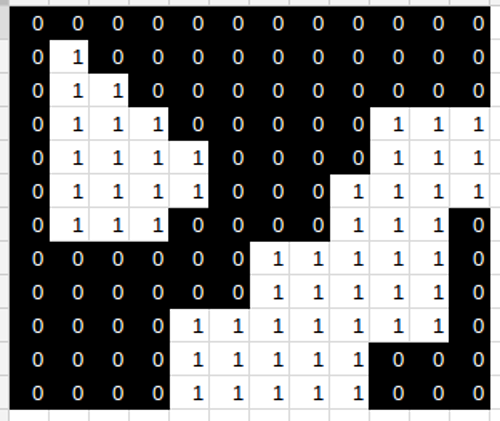
\includegraphics[scale=0.4]{pics/morphologyexample.png}
		\caption{Original Binary Image}
	\end{subfigure}
	\hfill
	\begin{subfigure}{.45\textwidth}
		\centering
		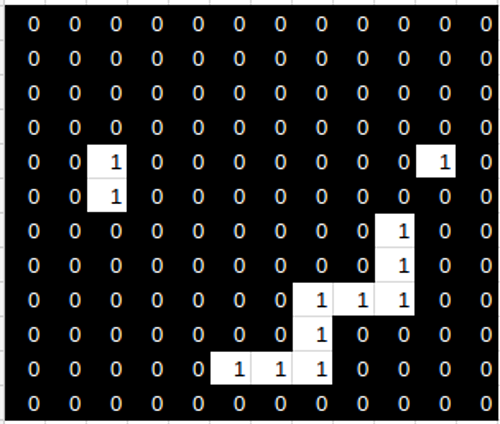
\includegraphics[scale=0.4]{pics/morphologyexample_e.png}
		\caption{Eroded Image}
	\end{subfigure}
	\label{fig:ErosionExample}
	\caption{Erosion}
\end{figure}

\subsubsection{Dilation}
\begin{center}
	Dilation causes bright areas of image to expand.
\end{center}

Dilation performs the opposite of what erosion would do. We still perform 
convolution with our 3x3 kernel but instead we set the pixel below the
kernel anchor to be the \textit{maximum} value within the 3x3 neighbourhood.
As a result, if there is even a single white pixel in the neighbourhood, the
current pixel will turn white. The only case this will not happen is if the 
pixel started off with a pixel value of 0 and all of its neighbours also had
a value of 0. Figure \ref{fig:DilationExample} shows the result of dilation with
the same original image as shown in the Erosion section above. 
\\
It can be observed from the result above that a dilation greatly increases
the size of the bright area. In addition, if bright areas are suitably close
to one another, it can cause the areas to join into a single, large
area as a result of applying the dilation.
This is how contours with small gaps are able to be closed and will aid in the
contour detection process. Again, the kernel size and shape may be changed to
cover a larger area (thus join bright areas further apart) or otherwise 
depending on how sensitive you want the operation to be.

\begin{figure}[H]
	\centering
	\begin{subfigure}{.45\textwidth}
		\centering
		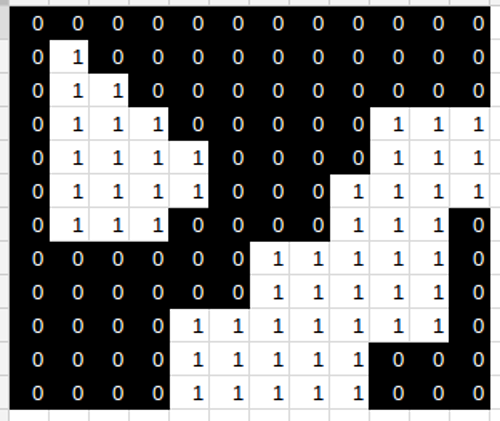
\includegraphics[scale=0.4]{pics/morphologyexample.png}
		\caption{Original Binary Image}
	\end{subfigure}
	\hfill
	\begin{subfigure}{.45\textwidth}
		\centering
		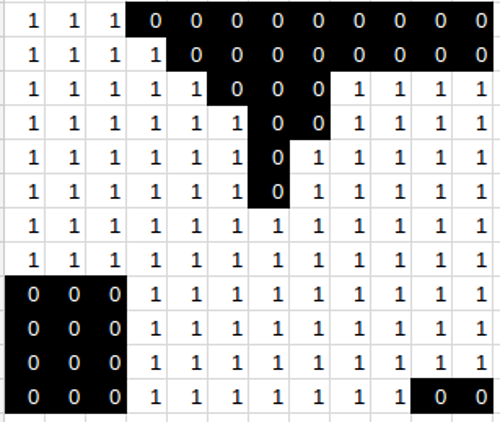
\includegraphics[scale=0.4]{pics/morphologyexample_d.png}
		\caption{Dilated Image}
	\end{subfigure}
	\caption{Dilation}
	\label{fig:DilationExample}
\end{figure}


\subsubsection{Morphological Closing}
\label{sec:morphologicalclosing}
\begin{center}
Morphological Closing is Dilation followed by Erosion.
\end{center}
Closing is very similar to dilation but it aims to preserve more information
about the original state and structure of the image.
The Closing operation is no different to erosion or dilation in that we
provide a kernel with which to convolve the given image with. To perform Closing,
the image first has a dilation operation applied to it with the given kernel. 
After this, erosion is done with the \textit{same kernel} on this dilated image. \\
By just performing dilation, we do manage to close small gaps in the image, 
however, every pixel is equally distorted by the kernel and so the resulting
image will look quite different to the original shapes, as can be seen
in the dilation stage in Figure \ref{fig:dilationstage}. 
In order to reduce as much
of this distortion as possible, erosion is used. The overall affect of this is
to make the resulting image as similar as possible to the shape of the
original image. Closing is idempotent, after one pass the resulting
image will not change from further Closings with the same kernel. The effect 
of closing is illustrated in Figure \ref{fig:closing}.\\
\\
The original images starts off with some holes within the image. If we
take this to be a contour discovered by an edge detector, then we can show
how we can close it with \textit{Closing}. After the Dilation stage, the
small holes within the original image have been closed, in addition, the 
boundaries of the bright parts of the picture have been joined due to their
proximity and the kernel shape. However, as seen in Figure \ref{fig:dilationstage},
the shape has changed a little from the original picture. After applying
erosion, seen in Figure \ref{fig:erosionstage}, the final result is much closer
in shape to the original picture, except it has its holes filled and the 
bright areas have joined. This would have closed the contour, if it were one,
preserving most of the original shape and not
losing too much fine detail through enlarging the bright area!

\begin{figure}[H]
	\centering
	\begin{subfigure}{.32\textwidth}
		\centering
		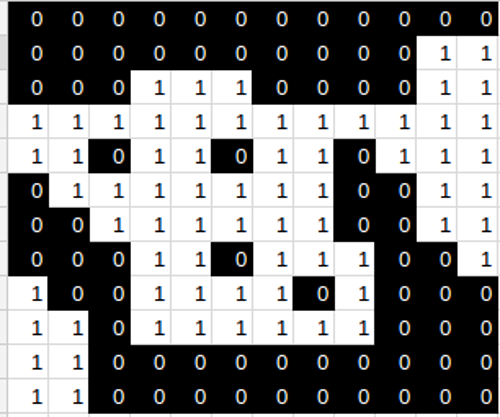
\includegraphics[scale=0.27]{pics/closing_o}
		\caption{Original Picture}
	\end{subfigure}
	\hfill
	\begin{subfigure}{.32\textwidth}
		\centering
		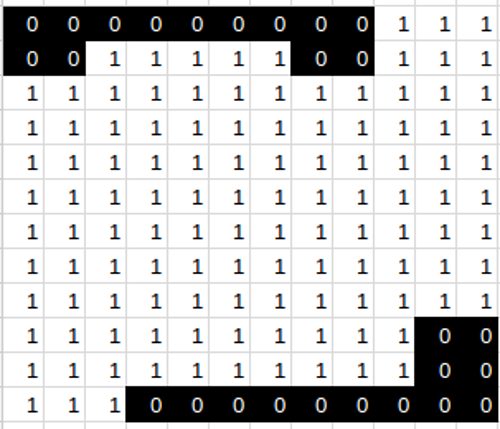
\includegraphics[scale=0.27]{pics/closing_d}
		\caption{Dilation stage}
		\label{dilationstage}
	\end{subfigure}
	\hfill
	\begin{subfigure}{.32\textwidth}
		\centering
		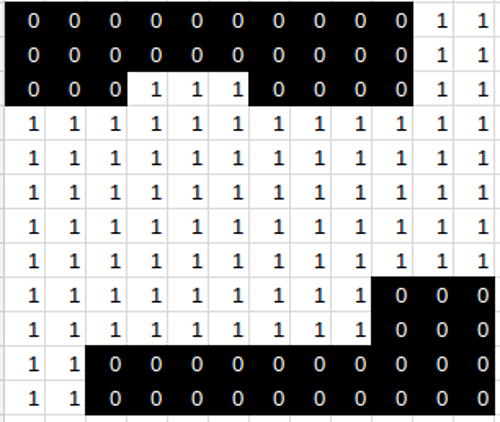
\includegraphics[scale=0.27]{pics/closing_e}
		\caption{Erosion stage}
		\label{erosionstage}
	\end{subfigure}
	\caption{Closing operator step by step}
	\label{fig:closing}
\end{figure}

\subsubsection{Image Differencing}
For users to be able to draw their own landscapes, there has to be some way
of recognising when there has been a change, physically, on paper. To 
automate this process enables the program to decide for itself when
there has been an update to a drawing, rather than a user having 
to confirm each time there is an update. Image differencing is the 
primary way of achieving this kind of detection. There are many 
different ways of actually
working out whether there is a "difference" between two images and some will
be further explained below. The general method for image differencing from
a video feed is taking two frames, one at time $t_s$ and a another at a 
time in the future $t_{s+c}$ and compare the two.

\subsubsection{Simple Intensity Differencing}
The simplest form of finding the difference between two images is comparing 
their pixel intensities. Equation \ref{eq:differencing} shows the typical
way of finding difference between two images, A and B. the equation 
simply states that the difference of a pixel is the difference in its 
intensity between the two images where:
\begin{itemize}
	\item[-] A is Image at time $t_{s}$
	\item[-] B is Image at time $t_{s+c}$
	\item[-] D is a \textit{Difference Image}
	\item[-] I(pixel) is a function returning the Intensity of the 
			supplied pixel.
\end{itemize}

\begin{equation}
		D_{i,j} = | I(A_{i,j}) - I(B_{i,j}) | 	
		\label{eq:differencing}
\end{equation} 

Once the Difference Image has been computed, performin a 
sum over all the pixels obtains an indication into how much "change"
there was. Depending on if the image is grayscale, binary or RGB will
give different ranges of change, the higher the range, the less
this final sum will be able to tell you about the change in the image as
total change can be attributed to several different factors.\\
\\
A popular way to deal with this problem is to first perform 
thresholding on the Difference Image before looking for total
change. This is explained in Rosin's Paper
\textit{Thresholding for Change Detection}\cite{Rosin}, in which he
refers to the Difference Image as a Difference Map. 
Again, there are different types of thresholding
such as Truncation, to-Zero, Binary and all of their inversions. 
For the purposes of this project, we will only look at Binary 
thresholding as it is the simplest way of representing change which
is in a yes or no fashion. \\
\\
Binary thresholding uses a threshold value, $\tau$, which is 
acquired either through statistical or empirical methods. With
the threshold, any pixel value in the Difference Image that is below
the threshold is effectively ignored and set to 0. The pixels above
the threshold are set to 1. This method is very quick,
especially when considering grayscale images where the range of
pixel values is between the value 0 to 255 and $\tau$ can be a hard
cut off point. It gets harder to use Binary thresholding with images 
with more colour channels as each colour channel may merit it's own
unique threshold, recquiring need to obtain $\tau_{1}, \tau_{2} .. \tau_{n}$
where $n$ is the number of channels in the image. 
Equation \ref{eq:differencingEq} describes thresholding in the grayscale 
case.

\begin{equation}
	D_{i,j} = 
	\begin{cases}
	0, & \text{ if $D_{i,j}$ $\leq$ $\tau$}. \\
	1, & \text{ otherwise}.
	\end{cases}
	\label{eq:differencingEq}
\end{equation}

By summing over these obtained values, the result may make more
sense as it is a representation of how many pixels in the image have
changed such that their change is significant. Of course this
"significance" is determined by the user and the chosen $\tau$.\\
\\
It is obvious that this is a very simple way of calculating difference
between images. To ensure accurate results, the camera has to stay
very still. If this is not the case, every pixel could experience a 
change in intensity as the pixture is no longer aligned. 
This can be somewhat countered by choosing
and appropriate $\tau$, depending on the change in the environment. 
However, if looking for finer changes, the
chosen $\tau$ could remove some of them, meaning an inaccurate and
undesirable detection result.\\
\\
In addition, if the images are taken in different lighting environments,
that too will cause inaccurate indications of difference. Take two
potential scenes, exactly the same and untouched with camera fixed. In
the day time, the image captured will have a much higher intensity
than an image taken in the evening, when it's dark. 
Comparing the two could cause the whole image
to be above the threshold of change but actually tell us nothing 
about changes in the scene, if any. In addition, if choosing a $\tau$ for 
a well lit environment will differ from a darker environment. This is because
as it gets darker, any added contours to the scene will cause a smaller
intensity difference as the scene is closer in tone to the dark colour
of the utensil used to draw the contour. In this case, even a large change
may not induce a large enough intensity change to signify a difference in the
scene. The problem with dealing with
illumination changes becomes more prominent in surveillance literature but
will not be much of a problem as described in Section \ref{sec:assumptions}
concerning my assumptions when creating this project.
A way to reduce the illumination effect is to perform a normalisation
of the pixels based on average intensities and variance. This shall
not be explained further but details and other detection 
techniques are highlighted it Radke's paper\cite{Radke04}.

\subsubsection{Image Ratioing}
Image Ratioing is another method to compare images. The general concept
is explained (along with other change detection techniques) in Singh's
paper \textit{Review Article Digital change detection techniques 
using remotely-sensed data}\cite{Singh88}. Again we have our two images,
from before, taken at different times. From here, the pixels' intensities
are compared to obtain a ratio, shown in Equation \ref{eq:ratio}:

\begin{equation}
	R_{i,j} = \frac{A_{i,j}}{B_{i,j}}
	\label{eq:ratio}
\end{equation}

The closer this $R_{i,j}$ values is to 1, the more similar the two 
pixels are in terms of intensity. Thus, if $R_{i,j}$ is quite far from 
1, it is a good indicator that there has been change within the image.
Again, thresholding can be applied to ths Ratio Image, $R$, which will 
leave only those with a significant ratio to be considered. The same steps
as image differencing can then be utilised to gain a representation of the
overall change in the image. The process, however, may introduce some error,
especially as you consider less of the electromagnetic spectrum. For example,
a grayscale image has values 0 to 255 per pixel. The ratio of a change from
3 to 1 is the same as a ratio change from 240 to 80 when the latter is clearly
a larger change in the intensity of the pixel. Instead, the ratios of the
pixels from several same images from different bands are used to determine
the ratio with the same equation as above. The image/spectral ratioing
algorithm, Singh uses in his paper utilises band 2 and band 4 images. The 
ratioing technique was criticised by Singh, he states: \\
\begin{quote}
The critical element of the methodology is selecting appropriate threshold 
values in the lower and upper tails of the distribution representing change 
pixel values.
\end{quote}

A certain amount of empirical testing is needed to obtain a good threshold.
The method has also been criticised due to the "Non-normal distribution upon
which it is based", i.e. a Non-Gaussian distributed image which is produced as 
the resultof ratioing as the areas on either side of the mode are not equal, 
making the error rates on both sides not equal.

\subsubsection{Camera distortion}
A vast amount of Computer Vision requires the use of a camera, whether to 
capture video or pictures. In Augmented Reality a camera is an absolute
necessity. However, cameras suffer from distortion
in the lens hardware of varying degrees, usually with relation to the quality
of the camera. Distortion is usually less in the more expensive and 
high end cameras. However, since these distortions are constants, we can
correct them in order to achieve undistorted images from our cameras.
There are three common types of distortion, these are classified as
\textit{Radial Distortion}, which occur from the spherical shape and
symmetry of a lens. Pixels away from the optical centre are distorted
in some way:
\begin{itemize}
	\item \textit{Barrel Distortion} \\
			Where images seem more magnified the further away from the optical
			axis (usually a straight line through the centre of the lens) 
			the pixel is. This causes lines to bend outward from the centre.
	\item \textit{Pin Cushion Distortion} \\
			The opposite of Barrel Distortion, where the image becomes more 
			magnified the closer you get to the optical axis. This type of
			distortion causes parts of the image to bend inward toward the 
			centre and optical axis.
	\item \textit{Moustache Distortion} \\
			A complex mixture of the two types of distortion, where by the 
			image seems to be Barrel distorted and as you start at the
			image centre but then turns into a Pin Cushion-like distortion
			as it gets further away.
\end{itemize}

Figure \ref{fig:distortions} shows these distortions.

\begin{figure}[H]
	\centering
	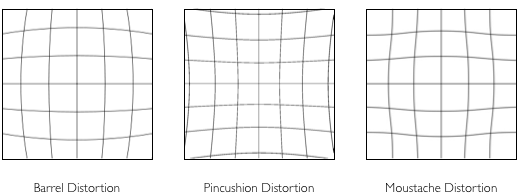
\includegraphics[scale=0.8]{pics/distortions.png}
	\caption{Lens distortion types}
	\label{fig:distortions}
\end{figure}

When working with Computer Vision algorithms, these distortions can cause
inaccuracies when analysing captured images. 
As a result, it is in our interest to find the transformations
necessary to counteract these distortions. Camera distortions only need to be 
calculated once as it will stay constant with the camera as the problem
is fixed in the hardware.
To undistort a camera image, we can use an image with known measurements 
as a reference to calculate the error rate of the camera, as well as
store these error coefficients. This is known as \textit{Camera Calibration}.
The coefficients should then be supplied
to any programs using the camera to obtain the data to correct the distortion.\\
\\
From a mathematical standpoint, there are intrinsics and extrinsic parameters
that describe the camera and its distortion from the real scene.\\
Intrinsic Parameters:
\begin{itemize}
	\item Focal length ($fx$ and $fy$, expressed in pixels)
	\item Optical center ($cx$ and $cy$, expressed in pixels)
	\item Distortion coefficients ($k_{1},k_{2}..k_{n}, p_{1},p_{2}..p_{n}$) which are
		indicators of tangential and radial distortion. Tangential distortion
		is caused when the lens is not parallel to the image plane and
		has to be correspondingly shifted. 
\end{itemize}

Extrinsic Parameters:
\begin{itemize}
	\item Rotation parameters ($Rx, Ry, Rz$)
	\item Translation parameters ($Tx, Ty, Tz$)
\end{itemize}

These parameters are arranged as transformation matrices and applied to the
image after it has been read by the camera to transform the image into
one that is undistorted.

\subsection{FINAL CHECK - Setting up the Camera and Environment}
To begin reading data from a video feed and manipulating it, there 
is a preliminary stage of setting up the correct environment. Here,
this means calibrating the camera and fixing the hardware into place.
In addition, to aid me in this project, I have used a few external
libraries that I will describe within this section.

\subsubsection{Camera Calibration and Setup}
It is important in the use of the program that the camera being used to
capture the scene is stationary. This is a fundamental restriction of the 
program. Althought it is possible to move the camera every so often,
most of the time it should be fixed to achieve the best results. The reason
for this being that if the camera is on an unstable surface or is constantly
experiencing some movement, the images captured will differ in pixels even though
the landscape image itself has not changed. This will cause continuous
recomputation of the landscape even though it does not need to be done. Extra
computation imposes unecessary extra costs on the hardware of the user's machine
and should be avoided. To user is permitted to move the landscape image in 
what direction they want, so long as it conforms the to restrictions
outlines in section \ref{sec:assumptions}.\\
\\
The camera used for this project was a webcam from Logitech, model C930e.
The webcam can be seen in Figure \ref{webcam}. The camera has 1080p HD 
recording with scalable video coding. It records at 30fps and has a wide 
angle view with autofocus. It was very easy to mount this webcam and start
using. The device is pretty high end, at the time of writing it is valued
at \$129USD which equates to around £85. Obviously this is not something
everyone can instantly get their hands on due to its cost, however, the
program will still function with much cheaper cameras, even in built
webcams on laptops will work too (however, angling these to face the 
landscape map while having the screen face the user is probably impossible).
However, this does prove that the webcam hardware is not a barrier to 
entry to start using this program to create landscapes. 

\begin{figure}[H]
	\centering
	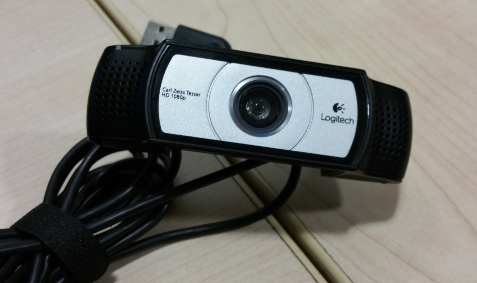
\includegraphics[scale=0.6]{pics/camera.jpg}
	\caption{Webcam used in this project: Logitech C930e}
	\label{webcam}
\end{figure}

To correct the issue of distortion within the web 
camera, I had to first calibrate it. This was
quite easily done by printing out a 7 by 5 square chessboard and running
OpenCV's provided calibration program. The calibration is a program included
within the OpenCV sample files and was run with the command:

\begin{verbatim}
./cpp-example-calibration 0 -w 6 -h 4 -s 0.025 -o ../cam\_0\_params.yml -op -oe
\end{verbatim}

The various inputs describe the nature of the board being used
for calibration. 6 and 4 are the number of internal corner points along
each side (squares per side $- 1$). The calibration process was very easy,
just running the program while moving the chessboard in front of the
camera in question, see Figure \ref{cameraCalibration} will create 
a YAML file containing the intrinisic camera data and information 
about its distortion. The YAML file can then be passed into the program to
help account for the the distortion and adjust the resulting displayed 
camera feed.

\begin{figure}[H]
	\centering
	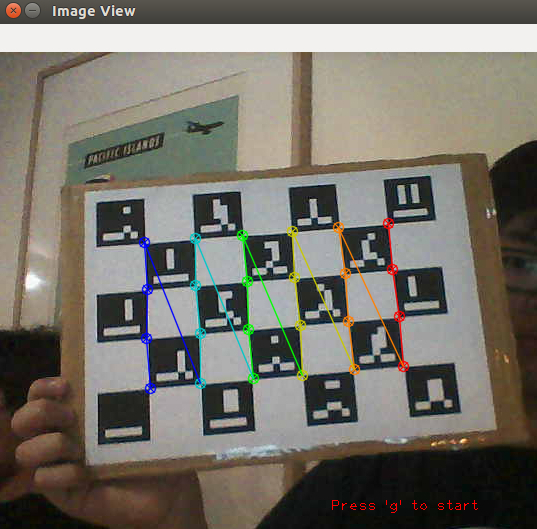
\includegraphics[scale=0.5]{pics/calibration.jpg}
	\caption{Calibrating the Camera}
	\label{cameraCalibration}
\end{figure}

\subsubsection{Choosing C++}
\begin{quote}
“C makes it easy to shoot yourself in the foot; C++ makes it harder, 
but when you do it blows your whole leg off.” - Bjarne Stroustrup
\end{quote}

C++ was the language of choice for this project.
As a project that was concerned with Augmented Reality, it meant that I was
definitely going to be messing around with Computer Vision to 
identify marker points and use Computer Graphics to then render objects over them.
In addition, it is a project that will be aimed at users of all kinds of ages,
anyone requiring a creative environment should be able to use the end product.
Augmented Reality is defined to have real time response and also requires custom 3D 
object generation and so will need to be very fast. Generally, this will mean
that I aim to use a language that can be immedaitely converted into native
machine code not something like Java that needs to be converted into Java byte code.
This project utilised the Computer Vision library
\textit{OpenCV} and the Computer Graphics Library \textit{OpenGL}. OpenCV is written 
C/C++ and has full support in C, C++, Java and Python, other language wrappers are
avialable such as C\#, Perl and Ruby. OpenGL supports various languages, however
since we are working on a real time program, we want a language that compiles
directly into machine code so that it is quick! As a result, the overlapping
language was C++ and was the chosen language to proceed with this project in.
C was the other alternative, although due to personal experience and Bjarne's
very relatable quote above, C also having a distinct lack of objects and 
containers lead me away from this choice. Even though there
were various problems along the way in terms of debugging, I consider
C++ the best, and probably only, choice of language.

\subsubsection{OpenCV}
OpenCV is the "Open Computer Vision" library, it is open source and was
developed by Intel in 1998. From the year 2000, it has been under the BSD
license, meaning it is a \textit{very} popular library to use. In addition,
it is probably the largest and most extensively used Computer Vision library.
OpenCV has a strong focus on real time applications, such as in video and
image processing. Some areas that
OpenCV is used in include Face recognition, Robotics, Motion Tracking, 
Augmented Reality and Interactions between Humans and Computers. In addition,
OpenCV also includes some statistical machine learning tools, aiding with
Decision Trees, KNN algorithsms, Naive Bayesian Classifiers amongst others. 
I shall not be utilising these in this project, however.\\
\\
OpenCV has various modules focused on different areas of
Computer Vision and offer numerous different transformations and operations
on images and video such as segmentation, edge detection, object tracking
amongst others. Kim Yu Doo's paper\cite{Kim14} has a very nice summary of
these modules that OpenCV offers. One of these is the recent GPU module which
allows computation to be done on the GPU to accelearate computation, this is
highlighted in K. Pulli's (senior Director at NVIDIA research) article  
\textit{Real-Time Computer Vision with OpenCV}\cite{Pulli12}.\\
\\
There were numerous other Computer Vision libraries available, such as 
the Cambridge Video Dynamics library (CVD) and CCV, though due to the extensive
documentation and usage of OpenCV along with its massive user and developer
community, it was obvious to choose it over these. 
Using the OpenCV library has plenty
of online documentation and guidelines. There are also numerous samples
that come along with the library that helped me get to grips with using it 
for my project. The version used throughout was OpenCV 2.4.11.

\subsubsection{OpenGL}
OpenGL, "Open Graphics Library", was introduced in 1992 and
developed by Silicon Graphics, supported by NVIDIA. 
It is the most widely adopted Computer Graphics Library. Akin to OpenCV, it
has a massive community and a lot of online help, along with a Wiki page to
support users. OpenGL interacts with the GPU to create computer graphics.\\
\\
When developing this project, I was using OpenGL Version 4.4, the most
recent version at the time of writing is version 4.5. With respect to this,
I saw no extra benefit in upgrading my version as it didn't offer anything
particularly useful to me. I simply needed the basic constructs
to generate a terrain and possibly map a texture over it.\\
\\
Some versions of OpenGL are limted based on what hardware (graphics card)
you have on your machine. I was using my personal laptop for the 
duration of this project which has an Integrated Intel Graphics card, along
with an NVIDIA GeForce 820M dedicated Graphics card which performs the 3D
rendering.\\
\\
Some of the code I wrote during this project is deprecated since the newer
versions. These started happening around OpenGL version 3.0, I did keep the
code as generous as possible to the lower OpenGL versions. In the event that
others use my code and they do not have a graphics card supporting
newer versions of OpenGL, they do not have to worry about their hardware 
requirements as I used functions that are common across even the very low
versions of OpenGL. For example, 
\texttt{glVertex()} and \texttt{glColor()} are two function calls I make in my
code but are now deprecated. It may be useful in the future to start moving
my code towards the replacement functions but that was one more worry
to include within this project which didn't really add much to the 
end goal. Since I have had exprience with ssaid functions before, 
that also made me favour sticking to the old function 
calls for the purpose of this project.

\subsubsection{ArUco}
ArUco is a C++ Augmented Reality library that offers wrappers and methods
based around OpenCV (versions 2.1 and above) that simplify the procedure
of identifying fiducial markers in an image. The library is under the BSD
license, created by the University of Cordoba in Spain. I am using the
most recent release of the library: version 1.2.5.\\
\\
ArUco has been used in a multitude of projects already with success and 
has helped me immensely in the creation of this project. The library 
allowed me to easily integrate a fiducial marker into the landscape map
and then detect this marker. Using properties of the marker, it was easy
to identify the orientation of the landscape map. The library is also 
pretty fast, however, it is worth noting that if this were to be ported
to mobile applications, ArUco currently performs much slower than on
computer, taking around 100 milliseconds to detect a marker, 
about 20 times slower than on a substandard processor like a Pentium 4.
Taking a look into the code, ArUco use the OpenMP API to parallelise
some of their code. This is probably on factor why it works much
slower on a mobile device which will likely have less processor cores, than
the typical computer.\\
\\
The ArUco library is also sufficiently documented, although more work can
be done in this area, it was enough to get me started. In addition, they
have a couple of example programs, some integrating with OpenGL, which 
allowed me to easily piece together a basic program that would render
an image over the fiducial marker in the scene. This would have been
a tough process otherwise due to the calibration of real world, camera and
3D model coordinate spaces which is handled nicely by ArUco.

\subsection{Capturing the Landscape map}
Now that the environment has been set up for the user, we begin the first
part of the Augmented Reality pipeline which is to conduct Computer
Vision algorithms on the scene the camera is capturing. This corresponds to
reading in the video feed of the landscape map that the user has drawn and
trying to understand it.

\subsubsection{Drawing the map}
To begin working with contour detection and landscape maps. 
I asked 2 friends, alongside
myself to draw potential landscape maps. I used these to test the
contour detection and this can be seen in my Evaluation in Section
\ref{chapter:evaluation}. Initially I worked based 
upon a static image basis, rather than using
video feed. The landscape maps were drawn on typical pieces of white paper with
black biro pen. The reason for using black biro pen is that it is the most
common utensil for the average person to use to draw or write things. 
Other utensils considered were pencils and black marker pens. 
Pencils will allow erasing parts of the scene, however, there will be 
gradient changes due to smudges and 
the effects of rubbing out pencil drawings. I decided to leave this 
scenario for a point later in the project or as an extension. 
Black marker pens are much thicker and thus easier
to detect by vision techniques, however, I did not want to limit users
to just black markers as they are not as commonplace as black biros.\\
\\
The images were drawn in specific ways, they can be viewed in Figure 
\ref{fig:landscapeMaps}. \\

\begin{figure}[H]
	\centering
	\begin{subfigure}[t]{.4\textwidth}
		\centering
		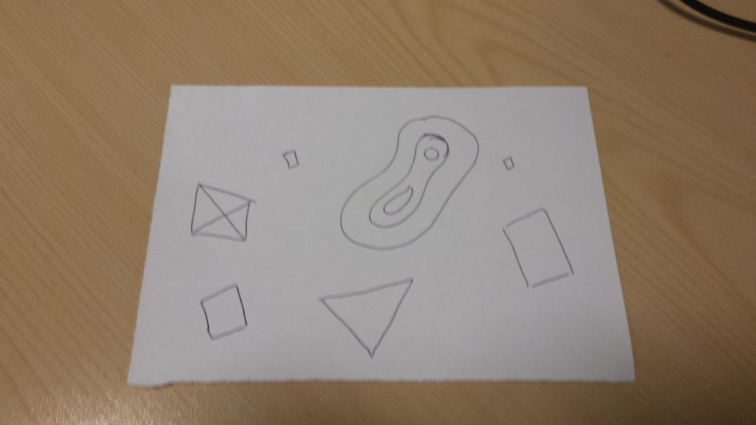
\includegraphics[scale=0.3]{pics/normal.jpg}
		\caption{A variety of contours and other shapes.}
		\label{fig:landscapeMapNormal}
	\end{subfigure}
	\hfill
	\begin{subfigure}[t]{.4\textwidth}
		\centering
		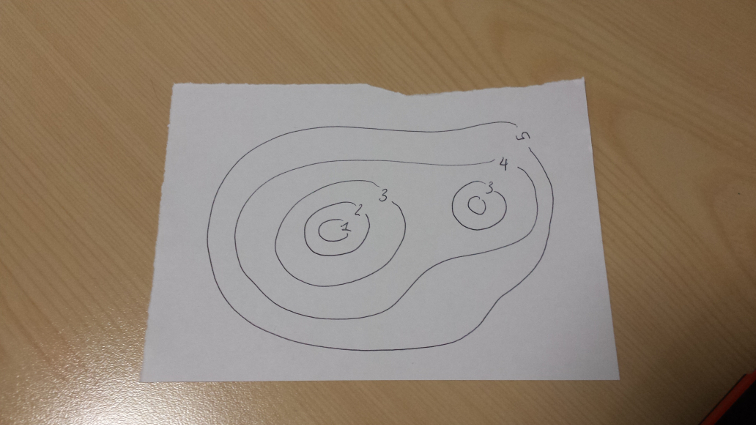
\includegraphics[scale=0.3]{pics/height.jpg}
		\caption{All contours open, no artifacts.}
		\label{fig:landscapeMapHeight}
	\end{subfigure}
	
	\begin{subfigure}[t]{.4\textwidth}
		\centering
		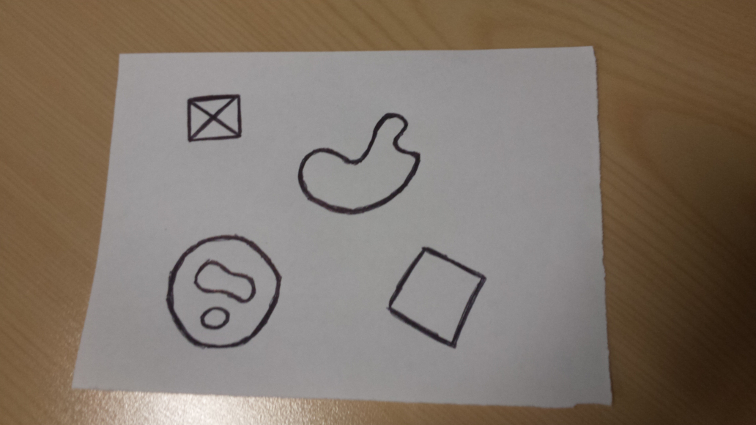
\includegraphics[scale=0.3]{pics/thicklines.jpg}
		\caption{Shapes and contours drawn in thickly, all closed.}
		\label{fig:landscapeMapThick}
	\end{subfigure}
	\hfill
	\begin{subfigure}[t]{.4\textwidth}
		\centering
		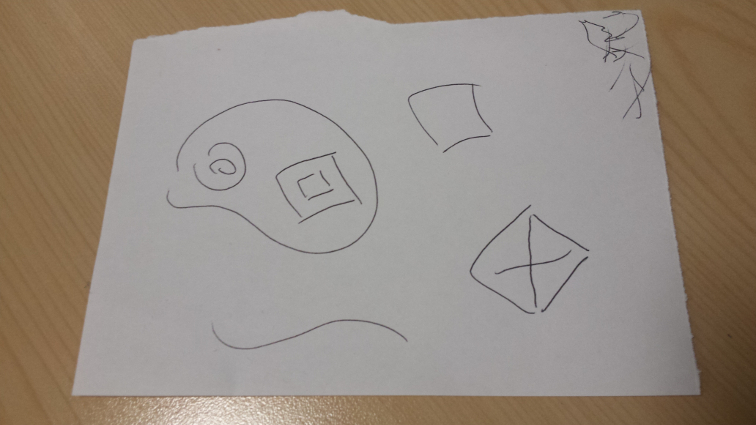
\includegraphics[scale=0.3]{pics/shitlines.jpg}
		\caption{Roughly drawn contours and pictures, som artifacts in the corner.}
		\label{fig:landscapeMapShit}
	\end{subfigure}
	
	
	\begin{subfigure}[t]{.4\textwidth}
		\centering
		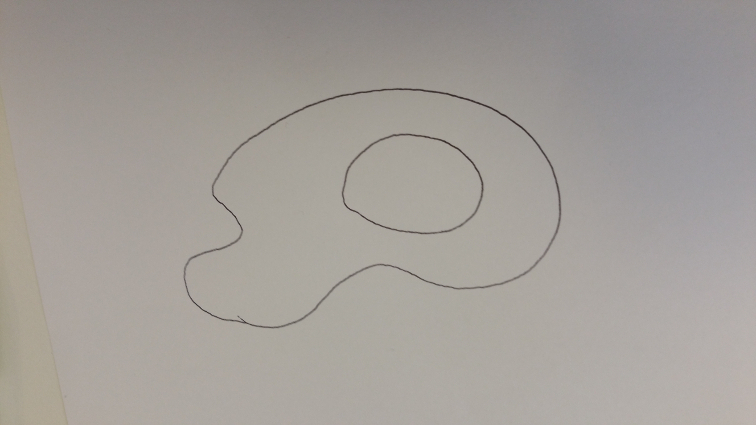
\includegraphics[scale=0.3]{pics/simple.jpg}
		\caption{Very simple contours drawn in; both closed.}
		\label{fig:landscapeMapSimple}
	\end{subfigure}
	\caption{Original landscape maps}
	\label{fig:landscapeMaps}
\end{figure}

Figure \ref{fig:landscapeMapNormal} has a couple of contours, closed, along with
a few other shapes. The contours have some small artifacts(some bold lines and
additional lines on the contour) which may happen in a typical drawing due to 
human error. The lines were drawn with intent, and although the other shapes are 
outside of the project's scope to identify as somethinig other than contours,
this picture was used to illustrate a "typical landscape map". \\
\\
Figure \ref{fig:landscapeMapHeight} was drawn by a friend who thought that 
labelling the contours with numbers to illustrate height would be a good idea.
Unfortunately, this is outside the scope of the project, we are following
the OS Map specification where each contour will dictate an uniform increase in
height, though without the added heights as all height will, by default, start
at 0. By doing so, the friend has created a bunch of open contours which were
used in this project to test the ability to close contours with small gaps. 
The ability to recognise numbers through template matching to manually set the 
heights may be a possible extension to this project but not something I will look
in to. \\
\\
Figure \ref{fig:landscapeMapThick} shows lines drawn in thickly, they are also
all connected. This represents a landscape map where the user may have used
a black marker or just thickly sketched out their design, making contour edges 
rough. This was made to mimic some noise as people may accidentally go over 
drawn lines and add small artifacts off the side of contours. 
Morphological Closing as well
as smoothing of the image with the Canny Edge Detector counter these small
artifacts.\\
\\
Figure \ref{fig:landscapeMapShit} tries to mimick a bad situation where
the user has drawn contours with large gaps, artifacts and other odd shapes
on the landscape map. There are also some scribbles in the top right corner, 
placed as a test to see how to what extent these would be captured. 
This drawing was more of a "lower bound" performance measure, to see
how limited the program would behave and could be done to remove human error
and what kind of restrictions and prerequisites a landscape map should have
to be cause a decent Augemented Reality rendering.\\
\\
Figure \ref{fig:landscapeMapSimple} is a very simple image. Two contours, one 
inside the other, both closed. This is the basic iage that could be used to
represent a "perfect" landscape map and is used to test how well the program
would work in the optimal conditions, if this isn't satisfactory, we cannot
expect any of the other drawings nor the user's drawings to perform well at all.\\
\\
Working on static images allowed me to mimic operating on frames taken from
a webcam. As a result, operating in this way allowed me to easily and quickly 
make adjustments to threshold parameters and other operations on the images
rather than having to extract from a camera each time and manually look at each
result generated was much easier to load the image and run several 
bash scripts which output all the image results to files I could quickly view.
I was very quickly able to attain empirical value for some of the thresholds
and parameters in the function calls that OpenCV offers, introduced
in the next section. I show how I evaluated the empirical value 
for the threhsolds in Section \ref{chapter:evaluation}.

\subsubsection{Detecting Contours}
Detecting contours is very simple when using OpenCV. A single function call
will perform Canny Edge detection, as outlined in the background of this report,
on the provided image. The function also performs double thresholding, so takes
two threshold values that I had determined empirically, along with an
aperture size for the Sobel operator and a choice of wether to use the L1 or L2 norm
when determining gradient magnitudes.\\
\\
The Canny function returns an image of contours. The image is 
passed to the \texttt{findContours()} function in OpenCV to obtain a set
of contours. These are represented as
a list of cartesian co-ordinates which dictate which pixels are considered part
of an identified contour. The method call in C++ is shown below.

\begin{lstlisting}
void Canny(img,contourImg,t1,t2,SAS,GMO)¶
\end{lstlisting}

\begin{enumerate}
	\item \texttt{img}: \\
		Input image where we are looking for contours within.
	\item \texttt{contourImg}: \\
		Is the resulting contour image produced by the algorithm.
	\item \texttt{t1}: \\
		Lower Threshold, part of Hysteresis as mentioned in 
		Section \ref{sec:Canny}. Contours with a strength higher than
		this value are considered "weak contours".	
	\item \texttt{t2}: \\
		Upper Threshold, second part of Hysteresis, mentioned in 
		Section \ref{sec:Canny} where contours of higher strength than
		this value are considered "strong contours".
	\item \texttt{SAS}: \\
		Sobel operator Aperture Size. The Sobel operator is used to 
		detect edges using gradient change and its size can be set here.
		The operator is a square of length set here.
	\item \texttt{GMO}: \\
		Gradient Magnitude Option, specifies how to compute norms of
		image gradient magnitude.
\end{enumerate}

The resulting \texttt{contourImg} is what is then passed onward to 
method \texttt{findContours()}. This will return a vector of vector
of points which describe the list on contours detected. This list
is further passed and used through the pipeline for more 
processing by Computer Vision methods. 

\subsubsection{Generating the Hierarchy Tree}
\label{sec:hierarchytree}
In openCV, there is a function that will take a contour image and from
it, figure out the points of the image that are on contours. The function is
called as below:
\begin{lstlisting}
void findContours(imgIn,contours,hierarchy,mode,method,p)
\end{lstlisting}

The variables \texttt{contours} and \texttt{hierarchy} are variables into which
the outputs of the function are placed. The \texttt{contours} variable is a vector
of contours, which themselves are represented as vectors of pixel points. 
The \texttt{hierarchy} variable is a list of all the contours and their
relation to the other contours (based on what is passed to the \texttt{mode}
variable in the method). I used \texttt{CV\_RETR\_TREE} to return a list which
describes a tree like hierarchy of the scene. Take for example the contour
image (computer generated for clarity) by the landscape map in 
Figure \ref{perfectsimple}.
The returned hierarchy is seen below (has been formatted for easier reading).

\begin{lstlisting}
hierarchy = [
	Contour 0: [-1, -1, 1, -1]
	Contour 1: [-1, -1, 2, 0]
	Contour 2: [-1, -1, 3, 1]
	Contour 3: [-1, -1, 4, 2]
	Contour 4: [8, -1, 5, 3]
	Contour 5: [-1, -1, 6, 4]
	Contour 6: [-1, -1, 7, 5]
	Contour 7: [-1, -1, -1, 6]
	Contour 8: [-1, 4, 9, 3]
	Contour 9: [-1, -1, 10, 8]
	Contour 10: [-1, -1, 11, 9]
	Contour 11: [-1, -1, 12, 10]
	Contour 12: [-1, -1, 13, 11]
	Contour 13: [-1, -1, 14, 12]
	Contour 14: [-1, -1, 15, 13]
	Contour 15: [-1, -1, -1, 14]
]
\end{lstlisting}

A contour is expressed in the following way:
\begin{verbatim}
Contour N: [Next,Prev,FChild,Parent]
Next = Next Contour on the same level as this contour (-1 if none)
Prev = Previous Contour on the same level as this contour (-1 if none)
Child = The first child contour of this contour  
         (a child is a contour contained within another contour)
Parent = the Parent contour of this one (-1 if none)
\end{verbatim}

\begin{figure}[H]
	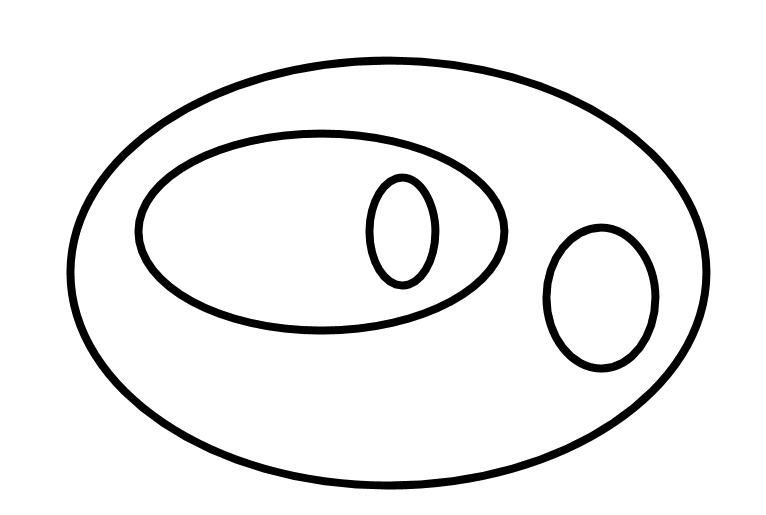
\includegraphics[scale=0.4]{pics/perfectsimple.png}
	\caption{Computer generated landscape map}
	\label{perfectsimple}
\end{figure}

To re-represent this hierarchy, I create a Tree Object that
encompasses the meaning of the hierarchy. The objects implementations
are shown below.

\begin{lstlisting}
class TreeNode {
public:
  //Methods and constructors removed
private:
  int level; //Level of the node in the tree
  TreeNode* parent;
  vector<TreeNode*>* children;
  TreeNode* next;
  TreeNode* prev;
  int nodeID; //ID of the node, as assigned by method findContours
};

class Tree {
public:
  //Methods and contructors removed
private:
  unordered_map<int,TreeNode*>* allNodes; //all nodes in this tree
  void insertNode(int TreeNode*);
};
\end{lstlisting}

I keep this hierarchy tree as a global object in the program that is used
whenever there is anything concerning contour manipulation. The tree is
also used when creating the 3D scene, explained in Section \ref{sec:3dgen}.

\subsubsection{~DO~ Joining Contours}
Joining contours is a key part of this project. As can be seen in the
section \ref{sec:hierarchytree}, the landscape map in Figure 
\ref{perfectsimple} produced 15 detected contours after being
passed to some OpenCV methods. Looking at the landscape map, it is
extremely clear to us humans that there are ony 4 contours present.
This means that Canny detection has probably split up each contour into
3 or 4 different contours that are very close but have gaps in between
preventing them from being considered as one full contour. The returned
hierarchy is thus not helpful to us at all as the realtionships between
contours is inacccurate. Our primary goal now becomes to join contours
before analysing any hierarchical data.\\
\\
\underline{Morphological Closing}\\
The first step to join contours is to perform morphological closing on 
the image. In Section \ref{sec:morphologicalclosing}, morphological closing 
was described as dilation followed by erosion. I do it in the opposite
way this time because we want the \textit{darker} areas (pen!) to expand
rather than the typical brighter areas to dilate.

\begin{lstlisting}
void morph_Closing(Mat* image, float elementSize, Mat* output){
  Mat structuringElement = getStructuringElement(MORPH_ELLIPSE,
	Size(elementSize,elementSize),
	Point(ceil(elementSize/2.0f), ceil(elementSize/2.0f)));
  Mat erodedImage(image->rows, image->cols,DataType<float>::type);
  
  erode(image, erodedImage, element);
  dilate(erodedImage,output,element);
}
\end{lstlisting}


\underline{Joining contours based on locality}\\
The next step is realising that sometimes, a single contour is split into
two but since they actually are both from the same contour, their end and
start points are very close. With this in mind, I implemented a 
\texttt{naiveContourJoin} function. The function call is shown below and
the corresponding algorithm shown in Algorithm \ref{algo:naivecontourjoin}.

\begin{verbatim}
vector<Point>* naiveContourJoin (vector<vector<Point> >*contourList, 
                         vector<vector<Point> >* joinedList)
\end{verbatim}

\begin{algorithm}
\DontPrintSemicolon
\Begin{
contourList is a vector of all contours, each contour is a vector of\;
points which make up the contour.\;
joinedList is the vector of returned contours.\;
\;
currentContour $\longleftarrow$ first contour in contours\;
\For{contour $in$ contours[1..$length($contours$-1])$}{
	\If{$adjacent($currentContour$,$contour$)$}{
		$join($currentContour$,$contour$)$\;
	}\Else{
		add currentContour to joinedList\;
		currentContour $\longleftarrow$ contour
	}
	add currentContour to joinedList\;
	update the Hiearchy Tree\;
}

}
\caption{Joining contours based on proximity of start and end points.}
\label{algo:naivecontourjoin}
\end{algorithm}

The function \texttt{naiveContourJoin} works by traversing the list of 
contours and examining in turn whether two contoursare adjacent, due to 
the nature in which OpenCV identifies contours, we can safely consider 
contours adjacent to each other in the list to check their adjacency. 
Adjacency is determined by whether the start or end of one contour is within
a certain area of the strat or end of another contour. If it is, the 
contours are joined, if not, we move on down the list.

.........................MORE(other methods)


.................FINISH, DO CONTOUR REMOVAL FROM Augmented RealityEA


\subsection{Generating the 3D scene}
\label{3dgen}
After the initial Computer Vision aspect of the program has been completed,
we can move onto the generation of the Augmented Reality scene that is
overlayed onto the camera feed so that the user is able to view the
landscape that they have drawn. From here, we have entered the Computer
Graphics portion of this Augmented Reality program pipeline.

\subsubsection{~DO~ View Point alignment}
Thanks to the ArUco library, there was little need to deal with the
complications of aligning camera coordinate space, rendering coordinate space
and real-world coordinate space together. Usually, there would be
need to align the Model, Projection and View matrices. The Model matrix
is the space in which our 3D graphics are rendered. The View matrix is
our camera, how we angle it and where it lies in relation to everything
else. The Projection matrix tells us what we will show on the screen,
until what depths we wiill view the image and what should be clipped.
In conjunction with this, there is also need to
to understand the relation of the Camera to World coordinates to appropriately
overlay the landscape on top of the correct part of the drawing.\\
\\
ArUco solves these issues in a few lines of code. 
After identifying the marker
locations and knowing the intrinsics of the camera, calling the following:
\begin{lstlisting}
	marker.glGetModelViewMatrix(modelview_matrix);
	cameraIntrinsics.getProjectionMatrix(proj_matrix);
\end{lstlisting} 

we obtain
the necessary matrices to pass to OpenGL to solve the coordinate space
alignment. By passing the matrics into OpenGL in their corresponding
matrix modes, I simply placed in my vertex and OpenGL primitive generation code.
However, the only catch is that the coordinate space is set by ArUco to have
an origin at the centre of the detected marker. Another point to note is
that the axes are scaled down to a size that is equivalent 
to the marker in the real world.\\
\\
In order to place the objects correctly in the scene, there was need to 
account for the fact that all generation is centred around the marker centre.
This was simply done by translating the model rendering coordinates by the
location of the marker centre
.............. ADD ABOUT HOW TO SCALE THE IMAGE TO THE CORRECT DIMENSIONS

\subsubsection{~DO~ From Hierarchy Tree to Height Map}
Taking the resulting hierarchy from the Computer Vision stage of this
program, we can then convert it into a height map which represents the
state of the landscape. The height map is then used later on in the pipeline
to help generate the landscape.\\
\\
Creating the hierarchy tree allowed me to gracefully attach tree
depths to each contour, encapsulated within a \texttt{TreeNode}. Thus,
all that needs to be done is identify the contour that each pixel resides
in and render its height as that equivalent to the depth of the 
\texttt{TreeNode} in the tree. However, this will create a massive "step"
landscape which means that where there is a contour boundary, the
pixels will suddenly jump from one height to another. This looks very
unrealistic and not aesthetically pleasing. Since anything concerning
computer graphics relies on looking good, it was a given to smoothen out
the landscape heights. This was done with Euclidean distance transforms 
in mind, where we increase the height of the pixel by a percentage of how
far the pixel is to the next height level. In essence, I implement a 
basic interpolation function that assigns a height as described in the 
pseudocode in Algorithm \ref{algo:assignHeights}.

\begin{algorithm}
\DontPrintSemicolon
\Begin{
\For{$h\in imageHeight$}{
	\For{$w \in imageWidth$}{
	p $\longleftarrow pixel(h,w)$\;
	c1 $\longleftarrow getContainingContour(p)$\;
	c2 $\longleftarrow getClosestContour(p,c1)$\;
	
	baseHeight $\longleftarrow getLevel(c1)$\;
	d2parent $\longleftarrow getDistanceFromContour(p,c1)$\;
	d2next $\longleftarrow getDistanceFromContour(p,c2)$\;
	extraHeight $\longleftarrow d2parent/(d2parent+d2next)$\;
	HeightMap[h][w] $\longleftarrow$ baseHeight + extraHeight\; 	
	}
}
}
\caption{Assigning heights to the pixels in the heightmap.}
\label{algo:assignHeights}
\end{algorithm}

However this algorithm depends on the function \texttt{getContainingContour}
which, though provided in OpenCV as \texttt{pointPolygonTest}, using
the function does not provide results as expected. The \texttt{findContours}
function, mentioned in \ref{hierarchytree} returns a contour list as
well as a hierarchy. Even though the hierarchy can be established, sometimes
\texttt{pointPolygonTest} doesn't recognise the contours as fully closed and
so will not return as expected.\\
\\
Another pitfall is depending on the \texttt{getDistanceFromContour} function.
OpenCV also provides this functionality through \texttt{pointPolygonTest},
yet the specified behaviour in the OpenCV documentation is that it 
"\textit{estimates the signed distance from the point to the nearest 
contour edge}". What this means is that if I were to use this function
to give me the height from one contour to another it would be inaccurate.
This is best illustrated in Figure \ref{fig:polygonTest}. 

\begin{figure}
	\centering
	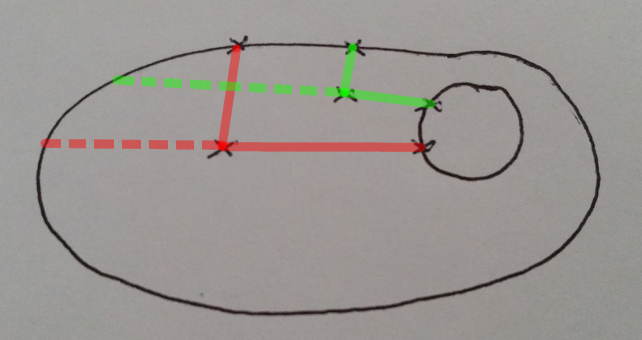
\includegraphics[scale=0.6]{pics/polygontest.jpg}
	\caption{Why not to use \texttt{pointPolygonTest}}
	\label{fig:polygonTest}
\end{figure}

In Figure \ref{fig:polygonTest}, there are two points contained within
the larger contour. To try and assign it a height, we need to know the heights
of the the contour it is contained in and the next highest contour. 
The points marked with a cross on each contour and connected to the
two considered points with a solid line represent the closest
point on the contour to them. If I were to take a proportion of total
distance to interpolate heights, as outlined in Algorithm 
\ref{algo:assignHeights}, the two points will be roughly assigned the 
same height due to the proportion of distances being the same. This is
not what is desired as the green point is clearly close to the next contour 
and should be higher. It would be more ideal to measure the closest distance
to the next contour and then follow that line to the containing contour, as
I have shown in the dotted line versions on the same figure. However,
OpenCV offers no easy way to do this and calculating it would be tedious,
making extra calls to \texttt{pointPolygonTest} for each pixel in the 
image, thus order $O(n^2)$. Of course, this is reasonable until there
are more child contours within the containnig contours as we'll have to
compute the shortest distances between them all and then work out the 
dotted line component.\\
\\
As a result, I offer an alternative algorithm, seen in 
Algorithm \ref{algo:assignHeights2}. The algorithm involves holding 3
matrices of equal size to the image. 

\begin{algorithm}
\DontPrintSemicolon
$baseLevelMap$ stores the level of the contour the pixel is within\\
$foundMap$ is a bitMap indicating which pixels are considered "found" by the
			algorithm\\
$explosionMap$ is a map of pixel distances to the next, closest, contour\\
contourList is a vector of vectors of points, each describing a contour\\
\Begin{
	Initialise $foundMap$ to all be $false$\;
	Initialise $explosionMap$ to all be $0$\;
	\For{contour $in$ contourList}{
		\For{point $in$ contour}{
			$foundMap($point$) \longleftarrow true$\;
		}
	}
	
	$currentHeightLevel \longleftarrow 0$\;
	\While{$foundMap$ has false entries}{
		\For{Each found point $\&\&$  
			$baseLevelMap($point$) = currentHeighLevel$}{
			set all neighbours of point to $true$ in $foundMap$\;
			increment $explosionMap($point$)$\;	
		}
		\If{all points that are $currentHeighLevel$ in $baseLevelMap$
			are true in $foundMap$}{
			increment $currentHeightLevel$\;			
		}
	}	
}
\caption{Corrected height assignment into the heightmap.}
\label{algo:assignHeights2}
\end{algorithm}

\subsubsection{~DO~ Landscape Generation}
Generating the landscape was not much of a problem after this stage. By
creating the \texttt{baseLevelMap}I can assign a height to all the pixels
already. However, doing so would make the terrain appear very step-like
rather than smooth. In an attempt to correct this, I create the 
\texttt{explosionMap} which gives a distance in pixels that a pixel 
is from the nearest contour pixel. From here, a simple proportion 
calculation can be used to work out the heights of each pixel. For 
example, if a pixel has an \texttt{explosionMap} value fo 30, it is 30 
pixels away from the next contour up. If the highest value in that
level is 36, then the height of the pixel is
$30 \div 36 + baseLevel$. I do this for all pixels in the 2D array
and store the heights.\\
\\  
All that remains past these steps is a simple 1-to-1 map of each
entry in the 2D array to a pixel point on the screen. I made use of
the openGL primitive, Quads, to generate the landscape. The code snippet
below in Figure \ref{quadcode} shows how I take use the height map 
to assign heights to each vertex of the quad, equivalent to the 
heights in the final 2D array.

\begin{figure}
\begin{lstlisting}
for(int i=0; i<WIN_SIZE; i++) {
  glBegin(GL_QUADS);        
  for(int j=0; j<WIN_SIZE; j++) {
    glColor3f(0.0f,(1.0f/finalHeightMap[i][j]),0.0f);          
    glVertex3f( float(i), float(j),finalHeightMap[i][j]);
    glVertex3f( float(i), (j+1.0f),finalHeightMap[i][j+1]);
    glVertex3f( i+1.0f, (j+1.0f),finalHeightMap[i+1][j+1]);
    glVertex3f( i+1.0f, float(j),finalHeightMap[i+1][j]);
  }
  glEnd();
} 
\end{lstlisting}
\caption{Assigning heights to Quad corners}
\label{quadcode}
\end{figure}

\subsection{Detecting change in the scene}
To provide the functionality of no user input, which was one of the main
focuses of this project, there has to be some way to indentify when it 
is time to redraw the scene. In this section I describe how I determine 
change within the landscape map and whether it is significant enough 
to represent a user change instead of a small change in environment.

\subsubsection{Generating the Base image}
\label{sec:baseimage}
The Base Image is the current landscape map that is used for generating the
Augmented Reality 3D landscape. This project was focused on providing 
users with a dynamically updating environment to tackle the problem that
some similar applications out there have, which is having to tell the program
when they want the scene rebuilt. For a creative individual, quickly and seamlessly
being able to make changes to their creation is paramount and a key motivation
for this project. Rendering the landscape over and over again based on
each frame is inefficient, and not really needed,thus I have implemented an 
algorithm that only requires re-render of a scene if there has been significant
enough change, i.e. the addition of a new contour.\\
\\
Right now, as the program starts, the first frame captured is considered to 
be the Base Frame. The Base Frame is held in memory and from there, 
constant comparisons to the subsequent frames are carried
out to determine whether significant change has been taken place. After a
threshold point, the Base can be considered to have changed and a new Base 
Frame will be stored. 

\subsubsection{~DO~ Introducing change}
Change in the landscape map occurs in two ways, it is also possible that
they happen simultaneously. The first way is by 
physically editing the landscape map. A user
can add and remove contours by drawing them in or erasing them from the 
scene. Removal of contours, however, will probably cause detection of
the other type of change which is positional change. When a user erases
a contour, they will likely shift the paper, when the user is not
erasing a contour, they may also rotate or move the paper around the camera
view.\\
\\
With each of these types of change, the scene has to be redrawn. Change
can also be introduced in other ways, some include obsuring of the scene
or the fiducial marker, drastic changes in illumination, objects
moving into the scene etc. However, with regards to 
Section \ref{sec:assumptions}, I assume that such unlikely and controllable
factors by the user will not occur and thus not cause problems in
change detection.\\
\\
However, I had to consider the event of small changes. This means slight
changes in the scene, i.e. say the user accidentally bumped the table on
which their camera sat, this causes a small misalignment in the camera.
Another scenario is that the user accidentally brushes the landscape map
with their hand and ever-so-slightly moves it from it's original position.
In cases similar to these, the change is so insignifcant that it hardly
demands a re-render of the scene and thus should not. Thus, to counter
this, I introduce various change thresholds which any change in the scene 
must surpass to count as adequate change for a redraw.

...................MORE (DO THE PICTURE TESTS AND THRESHOLDS)

\subsubsection{Determining Stabilisation}
The key part of creating the dynamic, self-updating environment
is determining when it is time to update. The reason for this
is that there should be an interval between a scene update that is 
not too frequent such that it imposes a large, unecessary amount of
computation on the system. In addition, 
we do not want it so infrequent that even after the user draws 
a new contour, there is still time before the recomputation occurs 
as this will take away from the real-time component whichh is so 
fundamental to Augmented Reality. A better way of choosing the time 
to update the 3D scene is to try determine \textit{when}
there has been a change in the landscape map.\\
\\ 
As mentioned earlier, the way I have chosen to do this is through 
a comparison of captured frames to an identified base frame. When 
there has been enough difference captured, we can say that this is
a suitable time to update the 3D scene and the base frame. 
However, the key here is to decide when we should actually update 
the base frame. There can be a massive change in the scene which
passes the threshold, for example, the user moving their hand into the
scene to draw in a new contour, every frame will be massively different
to the next due to the amount of movement going on in the scene. Thus,
the problem now becomes when can we say that the user has finished 
making edits to their masterpiece?\\
\\
The solution implemented was to look for stability. After substantial
change has occured, if the subsequent frames show little change, then
it is likely the user has finished their changes to the scene. Thus,
after this time has elapsed, we consider the first frame in the
examined sequence the new base frame and this will trigger a redraw of
the 3D scene. There are two ways in which change is identified in a base 
frame. These are between the landscape map or a change in the position
and/or orientation of the ArUco marker. 

\subsubsection{Generating a Difference Image}
Generating a Difference Image is rather simple. In the program, there is
a global variable, \texttt{BASEFRAME}, which is the current stored base frame.
Obtaining the base frame is explained in section \ref{sec:baseimage}. The
code for this is shown below and requires 3 simple calls to OpenCV 
functions. First, the base frame and the current frame are converted
into grayscale for ease of comparison. An absolute difference is calculated
between the two images, pixels with a difference higher than
\texttt{CHANGE\_THRESHOLD} are marked as they have changed significantly 
(as described by the threshold).

\begin{lstlisting}
	/*** Elsewhere in the code ***/
	//Converts into grayscale images
	cvtColor(BASEFRAME,gBASEFRAME, CV_BGR2GRAY);
	cvtColor(thisFrame,gthisFrame, CV_BGR2GRAY);
	/*****************************/

	//Create an image to store the Difference Image
  	Mat* diffFrame = new Mat(BASEFRAME.rows, 
  				BASEFRAME.cols,
  				DataType<float>::type) ;
	
	//Get the absolute difference between the base frame (note:
	//these are the grayscale versions) and the 
	//most recent frame, store this in the Difference Image.  				
  	absdiff(gBASEFRAME, gthisFrame, *diffFrame);	
  	
  	//Makes a binary image, pixels which have seen a change
  	//higher than CHANGE_THRESHOLD are set to 1, the others are 0.
  	//CHANGE_THRESHOLD is chosen empirically. diffFrame is the final
  	//binary image and can be used later.
  	threshold(*diffFrame, *diffFrame, CHANGE_THRESHOLD, 
  			MAX_COLOUR_VAL, THRESH_BINAugmented RealityY);
\end{lstlisting}

\subsubsection{Tracking the Fiducial Marker}
This step was rather easily taken care of. The library I used, ArUco, 
offered a very simple interface into the tracking of a fiducial marker(s)
in a given camera feed. The code to start it off is only a couple of 
lines.

\begin{lstlisting}
	MarkerDetector mDetector;
	cvtColor(inputImg,inputImg,CV_BGR2RGB);
	//remove distortion from frame
	undistort(inputImg,undistortedImg, 
		camParam.CameraMatrix, camParam.Distorsion);
	mDetector.detect(undistortedImg,markersList, 
		camParam.CameraMatrix,Mat(),markerSize,false);
\end{lstlisting}

Markers are stored in a list, \texttt{markersList}, which can then be 
iterated over to manipulate them individually. The library takes care
of orienting the markers such that even a through orientation of the
paper and reruns of the program, the markers are tracked consistently 
rather than corners randomly assigned. The markers are also identified
by using the Harris corner detection algorithm.\\
\\
Since we should only have one marker in the scene, this list will 
only grow to size 1. There is scope, to include more markers,
should this be a desirable thing. The library is said to perform
better the more markers there are in the scene that it can use for
stable identification. However, since it would be more ideal to have 
less additional markers in the scene for the purposes of this
project, this is probably not a good route
to go down.\\
\\
Another thing to note with fiducial markers is that since they have to be
in the scene as well, their edges will be detected. This means that it
will likely create a contour and have a landscape generated over it. This is
not the intention of the program and thus the contours created here will
have to be removed from the scene so that no landscape is generated there.
This is why achieving Augmented Reality without the use of explicit 
markers is an interesting topic. Ideally, we don't want to extra things 
in the scene which do not add to the 3D environment but are constants and
may be visually unappealing. If we didn't need the fiducial markers, it would
be one step closer to making Augmented Reality more "real". I did not
have time to try my fiducial marker removing ideas within this project,
I have outlined them in the Extensions Section \ref{chapter:extensions}.

\subsubsection{Detecting Stabilisation}
After figuring out how to detect change, all that remains is to use those
as ways to indicate stabilisation. Due to the sparse spread of code
for the project, I have instead included the pseudocode algorithm I 
used to detect stabilisation in the image, seen in 
Algorithm \ref{algo:stabilisation}. 

\begin{algorithm}[H]
\DontPrintSemicolon
BaseFrame is an image,\\
PotentialNewFrame starts off as equal to BaseFrame,\\
PotentialChange is a global flag,\\
StabilisedCounter is a global counter of frames.

\Begin{
\While{Camera is open}{
	thisFrame $\longleftarrow$ Next frame from Camera\;
	differenceImg $\longleftarrow getDifferenceImage(BaseFrame,thisFrame)$\;
	changedPixels $\longleftarrow countNonZero(differenceImg)$\;
	
	\If{changedPixels $>$ frame\_change\_threshold}{
		PotentialNewFram $\longleftarrow$ thisFrame\;
		PotentialChange $\longleftarrow true$\;
	}\ElseIf{PotentialChange is false}{
		StabilisedCounter++\;
		\If{StabilisedCounter $> $change\_requirement}{
			StabilisedCounter $\longleftarrow 0$\;
			BaseFrame $\longleftarrow$ PotentialNewFrame\;
			PotentialChange $\longleftarrow false$\;
			Redraw the scene\;
		}			
	} 
}
}
\caption{Detecting Stabilisation}
\label{algo:stabilisation}
\end{algorithm}

The logic behind the algorithm is as follows, from the base frame
each subsequent frame has the potential to become the new base frame, should
there be enough change between the two. Every time there is a significant 
difference between the last potential base frame and the next frame, the
potential base fram egets updated. If there are frames after the potential
base frame has been set that show change \textit{underneath} the threshold
then the stabilisation counter, \texttt{StabilisedCounter}, will be 
incremented. When \texttt{Stabilised Counter} has surpassed a set threshold
value, it indicates that there is high posibility that the scene has
settled from the last potential base frame update. What this translates
into is that it is likely the user has now moved their hand out of shot of the
paper and finished their change to the scene. When stability has been
achieved, a re-render of the scene and recaluclation of the hierarchy tree 
and height maps need to be done. Other stabilisation variables are reset for
next time a change might occur.

\subsection{Restructure and regenerating the 3D scene}
After a sufficient difference has been identified by the program, there is
now need to restructure and re-render the scene. This part of
the implementation did not require much work. All that needed to be done was
to take the new base frame that was obtained from the stabilisation
stage and create the new landscape from that. This is all encapsulated 
within one function call \texttt{createLandscape()} which changes
the global parameters, i.e. the height map and the hierarchy tree.\\
\\
The program is always in a continuous loop due to the \texttt{glutMainLoop()}
call. Since the scene is always rendered from the heightmap in each 
loop, once there has been a change and the new heightmap has been created,
the new scene will show to the user.\\
\\
Thus, with minimal extra work, the restructuring of the scene is done
after the stabilisation has occurred. By using two threads, one that
computes the new landscape after a base framme change, and the other
that runs the main glut loop, there is seamless update of the new
scene!

\section{Evaluation}
\label{chapter:evaluation}
In this section, I assess the outcomes of this project, trying to 
give numerical representation to its overall successes and failures.

\subsection{~DO~ Test Measures}
In Table \ref{fig:TestMeasureTable} below, I have compiled the various 
test measures I look into in an attempt to gain a representation of how 
well this project has turned out. For each, there is an associated 
unit of measurement in which I quantify the trait being assessed. 
The expected results correspond to what I originally considered the 
minimum result to be considered a success in that trait.

\newpage
\begin{landscape}
\begin{longtable}{p{.2\textwidth}|p{.2\textwidth}|p{.4\textwidth}|p{.25\textwidth}|p{.25\textwidth}}
\hline \hline
Trait to measure & Unit of Measurement & Reason & Expected Result & Actual Result \\
\hline \hline
Contour Detection &  Number of contours & A successful program will be able to 
										distinguish close to the real amount of 
										contours in order to accurately represent the	
										landscape map the user 
													has made      & Equal to drawing&  			  \\
\hline
Landscape Generation
	Accuracy     & By observation	   & Since the accuracy of the generation both
										 depends on how the end 3D scene looks in 
										 addition to being an accurate depiction of
										 the landscape map, the outcome should be 
										 judged from a user's viewing perspective
										        & Quite Smooth landscape,
										          all with heights as described by
										          the landscape map &  			  \\
\hline
Program Responsiveness &  Seconds      & Being real-time is a key part of Augmented
									  	 reality and so the response time between 
									  	 when the user has drawn the scene and when it
									  	 renders should be sufficeintly low to 
									  	 provide a real-time response
									  	        &    $<$ 2 seconds       &  			  \\
\hline
Base Frame 
   Stabilisation & By Observation	   & We want the program to re-render the scene
   										 only when an adequate amount of change has 
   										 occured and only when the scene has 
   										 stabilised. & Responds to an average contour    &  			  \\
              
                 &                     &        &                 &  			  \\
                 &                     &        &                 &  			  \\
                 &                     &        &                 &  			  \\                                                                                                     
                 &                     &        &                 & 
\label{fig:TestMeasureTable}
\end{longtable}
\end{landscape}
\newpage

\subsection{~DO~ User Testing}
%Being a creative, Augmented Reality environment for people to bring their 
%landscape creations to life, to assess its worth, there has to be feedback
%from the users. I chose an assortment of people from the Imperial College
%Computing Department to help test my application. In addition, I also
%got the younger siblings of my friends and peers to lend a hand as well! 
%I also looked to get feedback from those who are in the arts field,
%getting feedback from a handful of graphic designers and artists.

Below I have compiled some of the responses from the users who took part in
trying out this program. As well as their landscape maps and generated
3D landscapes.

\newpage
\begin{landscape}
\begin{longtable}{p{0.1\textwidth}| p{0.5\textwidth}| p{0.5\textwidth} | p{0.1\textwidth} |p{0.1\textwidth}}
\hline
User Landscape 		& Landscape Map 			& Generated 	& Run time(s) & Contours found vs actual\\
\hline
1. Student (Other)
	no artistic background & \begin{center}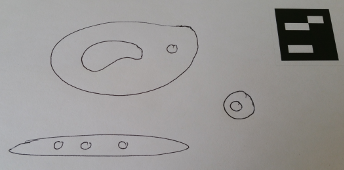
\includegraphics[scale=0.5]{pics/usertesting/1.png}\end{center} 
							& \begin{center}\end{center} & \\
\hline
2. Student (Computing)
	no artistic background & \begin{center}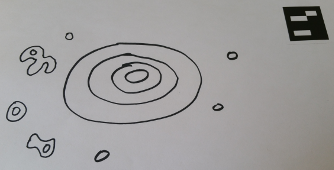
\includegraphics[scale=0.5]{pics/usertesting/2.png}\end{center} 
							& \begin{center}\end{center} & \\
\hline
3. Student (Computing)
	no artistic background & \begin{center}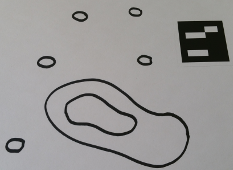
\includegraphics[scale=0.5]{pics/usertesting/3.png}\end{center} 
							& \begin{center}\end{center} & \\
\hline
4. Student (Computing)
	no artistic background & \begin{center}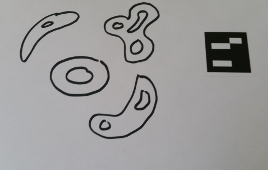
\includegraphics[scale=0.5]{pics/usertesting/4.png}\end{center} 
							& \begin{center}\end{center} & \\
\hline
5. Student (Other)
	no artistic background & \begin{center}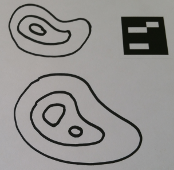
\includegraphics[scale=0.5]{pics/usertesting/5.png}\end{center} 
							& \begin{center}\end{center} & \\
\hline
6. Student (Computing)
	no artistic background & \begin{center}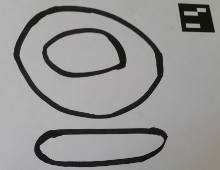
\includegraphics[scale=0.5]{pics/usertesting/6.png}\end{center} 
							& \begin{center}\end{center} & \\
\hline
7. Student (Computing)
	no artistic background & \begin{center}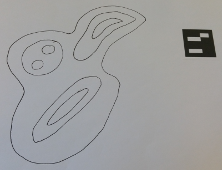
\includegraphics[scale=0.5]{pics/usertesting/7.png}\end{center} 
							& \begin{center}\end{center} & \\
\hline
8. Student (Computing)
	no artistic background & \begin{center}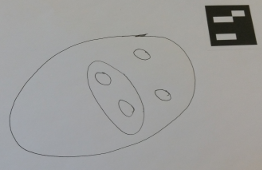
\includegraphics[scale=0.5]{pics/usertesting/8.png}\end{center} 
							& \begin{center}\end{center} & \\
\hline
9. Student (Computing)
	no artistic background & \begin{center}\includegraphics[scale=0.5]{pics/usertesting/9.png}\end{center} 
							& \begin{center}\end{center} & \\
\hline
10. Student (Computing)
	no artistic background & \begin{center}\includegraphics[scale=0.5]{pics/usertesting/10.png}\end{center} 
							& \begin{center}\end{center} & \\
\hline
11. Student (Computing)
	no artistic background & \begin{center}\includegraphics[scale=0.5]{pics/usertesting/11.png}\end{center} 
							& \begin{center}\end{center} & \\
\hline
\caption{A table arranging  images}
\label{tab:gt}
\end{longtable}
\end{landscape}
\newpage

\subsubsection{~DO~ Responsiveness}
There are different types of responsiveness that I wish to assess of this 
project. The first of which is the program's responsiveness to change (and
non-change) within the landscape map and developing environment. As the
main goal of the project, I will assess to what degree the program will
begin responding to change in the landscape map, in addition, 
\textit{how} it responds, for example to rather unexpected change in the
scene. The tests I have outlined for this section are the following:
\begin{itemize}
	\item No change introduced
	\item Small smudge/line (thick/thin) drawn
	\item Moderate (thick/thin) line drawn 
	\item Small (thick/thin) contour drawn
	\item Large (thick/thin) contour drawn
	\item Slightly open (thick/thin) contour drawn
	\item Open contour (thick/thin) drawn
	\item Illumination changed
	\item Contour drawn in similar colour to surface
	\item Rotation of the landscape map (thick/thin) 
	\item Translation of the landscape map (thick/thin) 
	\item Tilt of the landscape map (thick/thin) 
\end{itemize}

Most of the tests will be conducted twice, once with thick contours,
for example drawn with a permanent marker. The other test will be
with a thinner contour, i.e. drawn with a biro.

In addition, responsiveness can also be measured in terms of speed, rather
than detection. I also assess how quickly the program can respond
to changes in the scene. With this measure, there are significantly
less variables, I will test the following:

\begin{itemize}
	\item Time to respond to rotation
	\item Time to respond to translation
	\item Time to respond to tilt
	\item Time to respond to a new contour drawn
	\item Time to respond to a new contour drawn that affects the hierarchy
	\item Time to respond to an entirely new landscape map
\end{itemize}

\subsubsection{Aesthetics}
\begin{center}
	Aesthetics: A set of principles associated with the appreciation of beauty
	of an object, particularly in art. 
\end{center}

As this is a project which has a visual output, it is worthwhile to
judge the solution on how it looks/performs. Since beauty is 
sometimes said to be in the eye of the beholder, I have also accumulated
responses from other people (those who have no prior bias or association
to myself, the project or the Computer Science in particular).\\
\\
In this section, I will assess the following: How the generated landscape
looks, how did the result stack up against how the user envisioned their
landscape map and how nice the idea and set up of the project was.\\
\\
\underline{The Generated Landscape Aesthetics}\\
The generated landscapes seen from the user testing section above show
the extent of the aesthetics achieved in this project. Quite simply,
the generated graphics are not particularly pleasing. They describe the
scene and generally take the shape of what the user has drawn. The
colours of the contour areas accurately describe the height difference
in the image. However, the actual landscapes are still rather blocky. This is
a result of not being able to succesfully solve the double contour problem
of OpenCV detecting 2 contours for every 1 contour drawn. It is 
also partly attributed to the fact my solution to the problem uses
a discrete method to interpolate heights. Though I tried to correct this by
reducing the effect of discrete steps, it still is not enough to consider
the landscapes to be aesthetically pleasing. \\
\\
The landscapes could have been made a lot more appealing had I the time
to implement texture mapping or devised another way to assign heights.
Adding local illumination and surface normal points to the OpenGL Quads
I produced would also have given a better effect visually. These will
be outlined in the Extensions of this report in Section \ref{chapter:extensions}.\\
\\
\underline{Comparing Aesthetics of Idea to Reality}\\
The successful part of the aesthetics of this project is thaton successful
render, the created scene reflects the landscape map well, in terms of 
height, it matches up to what the user was thinking. However, the quality 
of the landscapes created compared to the vision each user had ended
up being lackluster as a general point of feedback. The reason for this
is that nowadays, with the amount of realism in Computer Graphics,
particularly games and entertainment, people have a base level of
realism they feel should be a given. As a result, the expectations
of the landscapes the users had in their mind whilst drawing the 
landscape map are expected to be of much higher quality. Given more time
with this project, such expectations may be able to be met. \\
\\
Although the quality of the landscapes wasn't the main
aim of this project, it is a worthwhile point to make about Augmented
Reality applications as a whole and definitely a point worth
evaluating and looking into for the future. If Augmented
Reality applications are to be used commercially, be
interesting and captivate users, they have to meet certain realism 
benchmarks that people implicitly create from exposure to 
Computer Graphics in their everyday life.

\subsection{Process Evaluation}
In this section I take time to evaluate my implementation process, aside
from the results gathered from the final product.

\subsubsection{OpenCV}
Using third party libraries is always a gamble, their performance is not
always guaranteed. Even for a library so well supported as OpenCV, there 
were times where the library did not behave as expected. This can be 
attributed to some of the algorithms used in the functions provided. 
Whether there exists a more suitable and better performing algorithm is
unlikely and hard to determine.\\
\\
Having justified my use of the OpenCV library, playing around with a 
few functions and digging through the documentation to see what was
on offer for me, I think it was the best option to use. 
However, I did not conduct a thorough enough investigation into specific
functions and their behaviour. This would have merited a lot more time in 
the beginning of the project, it would not have changed my mind to  use
the library but would have prepared me against some of the problems that 
arose throughout the project. The Computer Vision aspect is the most
important part in my project, it is the first step and an inaccurate
representation of the drawn scene will cause the rest of the 
implementation and the result to be inaccurate and essentially useless. As
a result, OpenCV played a huge part in this project. 
In this section, I outline some of the
problems that came with using OpenCV, a brief explanation of my solution
(of which more can be read about in Section \ref{lol}), and evaluation of
the solution. 

\subsubsection{Contour Detection}
The first major step in this project is contour detection. This was achieved
using the Canny Detector from OpenCV, thresholding empirically. Having
researched edge detectors avaiilable to me before hand, I was aware of those
available and I could manipulate the output in various ways by
changing the paramters passedto the function. I did experiment with different
sizes of Sobel kernel, which were 3x3, 5x5 and 7x7. In addition, I also
tested various upper and lower thresholds which are used for hysteresis. The
results were accumulated as pictures and I stored the output for visual
comparison. After this process was done I made my choice of threshold values
and kernel size based on which pictures seemed to capture the contours
in each contour the best. \\
\\
Figure \ref{fig:kernelDetermining} shows the way I determined the best kernel
size. I simultaneously raised the Upper and lower thresholds alongside the 
kernel size so that I could visually compare them later on. I did this
across different pictures as well, with different styles of contours drawn,
thick, thin, open etc. The Sobel operator has a smoothing effect when
used and so its size will affect contour detection quality.
From this I found that the best kernel size to use was
a 5x5 kernel. The best picture to illustrate this is \ref{kernelExample1} 
and \ref{kernelExample2}, Looking at the smaller, circular contour in
\ref{kernelExample1}, it is coloured red, with its inner contour
blue and then the inner contour's inner area coloured red. This highlights
3 distinct contours identified. In \ref{kernelExample2} the same contour
now only has two colours, the outer most being blue with the inner, inner
area being red. This is because the inner contour has been joined with the
outer contour as the kernel size was too large and determined the two
contours to be connected! In the other case, in \ref{kernelExample3}, the
same contour did not have its inner, inner area coloured, this  because the
kernel size was too small and did not join the contour completely. In 
addition, the simple square in \ref{kernelExample3}, just to the top right of
the large, curved contour, has its edges coloured green
and red, whilst both \ref{kernelExample2} and \ref{kernelExample3} correctly
detect the square to be one contour, coloured in a single colour. Since
the program should be able to tolerate some small amount of openness of
contours, the kernel size was determined, empirically, best of size 5.\\
\\
Figure \ref{fig:hysteresisDetermining} shows a
small selection of results I obtained through this kind of testing. After
seeing that performance was best between an upper threshold of 1700 and 2200,
along with a lower threshold of 800, I did a smaller scale, binary search
approach to reach the upper and lower thresholds the program currently uses
of 2000 and 900 respectively.

\begin{figure}[H]
\centering
	\begin{subfigure}[t]{.25\textwidth}
		\centering
		\includegraphics[scale=0.3]
		{pics/shitlinesThreshTest/Upper1700lower1000kernel3.png}
		\caption{U:1700, L:1000, K:3x3}
	\end{subfigure}
\hfill
	\begin{subfigure}[t]{.25\textwidth}
		\centering
		\includegraphics[scale=0.3]
		{pics/shitlinesThreshTest/Upper1700lower1000kernel5.png}
		\caption{U:1700, L:1000, K:5x5}
	\end{subfigure}
\hfill
	\begin{subfigure}[t]{.25\textwidth}
		\centering
		\includegraphics[scale=0.3]
		{pics/shitlinesThreshTest/Upper1700lower1000kernel7.png}
		\caption{U:1700, L:1000, K:7x7}	
	\end{subfigure}


	\begin{subfigure}[t]{.25\textwidth}
		\centering
		\includegraphics[scale=0.3]
		{pics/shitlinesThreshTest/Upper2200lower800kernel3.png}
		\caption{U:2200, L:800, K:3x3}
		\label{kernelExample3}
	\end{subfigure}
\hfill
	\begin{subfigure}[t]{.25\textwidth}
		\centering
		\includegraphics[scale=0.3]
		{pics/shitlinesThreshTest/Upper2200lower800kernel5.png}
		\caption{U:2200, L:800, K:5x5}
		\label{kernelExample1}
	\end{subfigure}
\hfill
	\begin{subfigure}[t]{.25\textwidth}
		\centering
		\includegraphics[scale=0.3]
		{pics/shitlinesThreshTest/Upper2200lower800kernel7.png}
		\caption{U:2200, L:800, K:7x7}
		\label{kernelExample2}
	\end{subfigure}


	\begin{subfigure}[t]{.25\textwidth}
		\centering
		\includegraphics[scale=0.3]
		{pics/shitlinesThreshTest/Upper2200lower1200kernel3.png}
		\caption{U:2200, L:1200, K:3x3}
	\end{subfigure}
\hfill
	\begin{subfigure}[t]{.25\textwidth}
		\centering
		\includegraphics[scale=0.3]
		{pics/shitlinesThreshTest/Upper2200lower1200kernel5.png}
		\caption{U:2200, L:1200, K:5x5}
	\end{subfigure}
\hfill
	\begin{subfigure}[t]{.25\textwidth}
		\centering
		\includegraphics[scale=0.3]
		{pics/shitlinesThreshTest/Upper2200lower1200kernel7.png}
		\caption{U:2200, L:1200, K:7x7}
	\end{subfigure}
	
	\caption{Example of determining Kernel size \\
		(U = UpperThreshold, L = LowerThreshold, K = KernelSize)}
	\label{fig:kernelDetermining}
\end{figure}

\begin{figure}[H]
\centering
	\begin{subfigure}[t]{.25\textwidth}
		\centering
		\includegraphics[scale=0.3]{pics/normalThreshTest/Upper1700lower800kernel5.png}
		\caption{U:1700, L:800}
	\end{subfigure}
\hfill
	\begin{subfigure}[t]{.25\textwidth}
		\centering
		\includegraphics[scale=0.3]{pics/normalThreshTest/Upper1700lower1200kernel5.png}
		\caption{U:1700, L:1200}
	\end{subfigure}
\hfill
	\begin{subfigure}[t]{.25\textwidth}
		\centering
		\includegraphics[scale=0.3]{pics/normalThreshTest/Upper1700lower1400kernel5.png}
		\caption{U:1700, L:1400}	
	\end{subfigure}


	\begin{subfigure}[t]{.25\textwidth}
		\centering
		\includegraphics[scale=0.3]{pics/normalThreshTest/Upper2200lower800kernel5.png}
		\caption{U:2200, L:800}
	\end{subfigure}
\hfill
	\begin{subfigure}[t]{.25\textwidth}
		\centering
		\includegraphics[scale=0.3]{pics/normalThreshTest/Upper2200lower1400kernel5.png}
		\caption{U:2200, L:1400}
	\end{subfigure}
\hfill
	\begin{subfigure}[t]{.25\textwidth}
		\centering
		\includegraphics[scale=0.3]{pics/normalThreshTest/Upper2200lower2000kernel5.png}
		\caption{U:2200, L:2000}
	\end{subfigure}

	
	\begin{subfigure}[t]{.25\textwidth}
		\centering
		\includegraphics[scale=0.3]{pics/normalThreshTest/Upper2700lower800kernel5.png}
		\caption{U:2700, L:800}
	\end{subfigure}
\hfill
	\begin{subfigure}[t]{.25\textwidth}
		\centering
		\includegraphics[scale=0.3]{pics/normalThreshTest/Upper2700lower1400kernel5.png}
		\caption{U:2700, L:1400}
	\end{subfigure}
\hfill
	\begin{subfigure}[t]{.25\textwidth}
		\centering
		\includegraphics[scale=0.3]{pics/normalThreshTest/Upper2700lower2000kernel5.png}
		\caption{U:2700, L:2000}
	\end{subfigure}
	
	\caption{Example of determining hysteresis thresholds with kernel size = 5. \\(U = UpperThreshold, L = LowerThreshold}
	\label{fig:hysteresisDetermining}
\end{figure}

A regret I have with the way I tackled detecting contours is not fully 
investigating using pure thresholding to identify contours. Quite naively, 
after reading
up the Canny edge detector versus other edge detection algorithms, I tunnel
visioned on that solution because I thought it was the best of the edge 
detectors. However, I did not consider the thought of not using
a edge detecor, just simply using a thresholding algorithm that if pixels 
vary in intensity from those nearby, mark it as a possible contour. I
missed the fact that I could purely use thresholding to identify possible
contours and use the result to form a hierarchy. However, in retrospect,
whether this approach would have worked better than using the Canny 
remains to be determined. It may
have behaved a lot worse, I would also have to spend a lot of time 
empirically determining the threshold values, especially without the 
use of hysteresis which is so useful in the Canny Edge Detector. However, if
the user was limited to using just black pen on a white paper surface,
detection of contours may have done well in the thresholding case. However,
with these points in mind, I think it was sufficient to try out the 
Canny detection method, due to its proven good performance by using
the double thresholding method with hysteresis. Detecting contours
without an edge detector could be a worthwhile extension or something that
future projects should consider in their approaches.

\subsubsection{Contour Joining}
OpenCV offers a method, \texttt{findContours()} which will return a
vector of contours (expressed as a vector of constituent points) along with
a hierarchy describing the relation of these contours. However, detection
isn't always perfect sometimes a contour, though continuous on paper
will be identified as several contours. In an attempt to reduce this, I 
use morphological closing to try connect contours as much as possible.
This worked to some extent but had to be amplified with another join
algorithm. The algorithm I implemented was to analyse the beginning and end points
of each contour, due to the order in which OpenCV discovers, it is sufficient 
enough to join contours that are subsequent to others in the returned
vector. If two adjacent contours are within an empirically set pixel
neighbourhood they will be joined together. \\
\\
When using the \texttt{findContours()} if a contour is not closed,
points, in an effort to close the contour, the library will duplicate 
points as a way to get from the end of the contour back to the beginning
point without loss of information. However, sometimes the backtrack does
deviate from the original beginning-to-end point path and choose a very
slightly different path on the way back to the beginning point. This causes 
a variety of complications, if we were to naively remove duplicate points
within each contour, there may be stray points on the contour that do not
belong. This is best explained in the example below in Figure \ref{backtrack}.
The coloured pixels indicate a possible contour. Consider this contour
starting left and ending right, this is not a closed contour and
so OpenCV tries to close it. The mauve pixels are pixels that are part
of the front and back traversal. On the way back the constituent pixels
deviate slightly due to detection in OpenCV. The black pixels are
on the path left to right, the pink pixels are those on the path right to left.
By eliminating duplicates, we will keep the pink pixels. If these are on the
way back and pixel discovery order is preserved, then the pink pixels are
where the contour will "end" as determined by OpenCV rather than at the 
original start point. This causes a massive problem later on where we
will be unable to tell if contours are actually closed or not and connecting
nearby contours becomes a problem since they no longer have their
start and end points nearby each other. \\
\\
After assessing the behaviour of 
the program after trying to eliminate duplicate points in conjunction 
with my \texttt{naivecontourjoin()} algorithm, I found these exact
problems to occur, making joining contours almost impossible. As it
would be better to reduce the amount of contours by joining them, my approach
to this problem was to simply leave the duplicated points as they would 
at least preserve the original contour end and begin properties. This is
something that should be considered by others thinking of working with
OpenCV for contour detection.

\begin{figure}[H]
	\centering
	\includegraphics[scale=0.8]{pics/backtrack.png}
	\caption{Contour Backtracking problem}
	\label{backtrack}
\end{figure}

\subsubsection{Contour Elimination}
For the landscape seen in Figure \ref{eliminationInput}, the results of
runnig \texttt{findContours()} can be seen in 
Figure \ref{fig:contourElimination}. In Figure \ref{eliminationInput}, we
clearly see that there are only 3 contours, OpenCV finds 21 contours. These
can be attributed to the fact that contours are counted twice (once entering
the contour, once leaving the contour) in addition to the ArUco marker being
treated as a contour. In addition, there are other contours found that are
a lot more subtle, some of these are joined with the \texttt{naivecontourjoin()}
algorithm as explained in the last section. Joining the contours
reduces the total count to 13 so my approach above does work quite well, but
there are still anomalies that will take more than just proximity checking
to join together. 

\begin{figure}[H]
	\centering
	\begin{subfigure}[t]{0.45\textwidth}
		\centering
		\includegraphics[scale=1.4]{pics/elimination.jpg}
		\caption{Landscape Map}
		\label{eliminationInput}
	\end{subfigure}
	\hfill
	\begin{subfigure}[t]{0.45\textwidth}
		\centering
		\includegraphics[scale=0.8]{pics/eliminationResults.png}
		\caption{Contours Found}
		\label{eliminationResults}
	\end{subfigure}
	\caption{Results of \texttt{findContours()}}
	\label{elimination}
\end{figure}

There were other algorithms implemented within this project to try to reduce the
contour count. This is because having a smaller contour tree will speed
up the overall computation in the program. The first of which was to try and
eliminate contours of negligible size. Looking at Figure \ref{eliminationResults},
we ca see cotour 9,10 and 11 have considerably less contours than the
other ones found, having under 60 points each. The original intuition is that
these can be thrown away with minimal impact on the understanding of the
landscape map. This is further backed up by the fact that they add
minimal extra value to the reconstruction of the landscape map in contour form,
which is seen in Figure \ref{construction}.\\
\\
As can be seen from Figure\ref{construction9}, Figure \ref{construction10} and
Figure \ref{construction11}. There is not much gained from keeping the smaller
contours. In addition, Figure \ref{construction12} also seems negligible, with
the final construction seemingly done by Figure \ref{construction8}. 

\begin{figure}[H]
	\centering
	\begin{subfigure}[t]{0.32\textwidth}
	\centering
		\includegraphics[scale=0.28]{pics/elimination/joinedAfterRemoval1.png}
		\caption{1}
		\label{construction1}
	\end{subfigure}
	\begin{subfigure}[t]{0.32\textwidth}
	\centering
		\includegraphics[scale=0.28]{pics/elimination/joinedAfterRemoval2.png}
		\caption{1,2}
		\label{construction2}
	\end{subfigure}
	\begin{subfigure}[t]{0.32\textwidth}
	\centering
		\includegraphics[scale=0.28]{pics/elimination/joinedAfterRemoval3.png}
		\caption{1,2,3}
		\label{construction3}
	\end{subfigure}
	
	
	\begin{subfigure}[t]{0.32\textwidth}
	\centering
		\includegraphics[scale=0.28]{pics/elimination/joinedAfterRemoval4.png}
		\caption{1,2,3,4}
		\label{construction4}
	\end{subfigure}
	\begin{subfigure}[t]{0.32\textwidth}
	\centering
		\includegraphics[scale=0.28]{pics/elimination/joinedAfterRemoval5.png}
		\caption{1 to 5}
		\label{construction5}
	\end{subfigure}
	\begin{subfigure}[t]{0.32\textwidth}
	\centering
		\includegraphics[scale=0.28]{pics/elimination/joinedAfterRemoval6.png}
		\caption{1 to 6}
		\label{construction6}
	\end{subfigure}

	
	\begin{subfigure}[t]{0.32\textwidth}
	\centering
		\includegraphics[scale=0.28]{pics/elimination/joinedAfterRemoval7.png}
		\caption{1 to 7}
		\label{construction7}
	\end{subfigure}
	\begin{subfigure}[t]{0.32\textwidth}
	\centering
		\includegraphics[scale=0.28]{pics/elimination/joinedAfterRemoval8.png}
		\caption{1 to 8}
		\label{construction8}
	\end{subfigure}
	\begin{subfigure}[t]{0.32\textwidth}
	\centering
		\includegraphics[scale=0.28]{pics/elimination/joinedAfterRemoval9.png}
		\caption{1 to 9}
		\label{construction9}
	\end{subfigure}

	
	\begin{subfigure}[t]{0.32\textwidth}
	\centering
		\includegraphics[scale=0.28]{pics/elimination/joinedAfterRemoval10.png}
		\caption{1 to 10}
		\label{construction10}
	\end{subfigure}
	\begin{subfigure}[t]{0.32\textwidth}
	\centering
		\includegraphics[scale=0.28]{pics/elimination/joinedAfterRemoval11.png}
		\caption{1 to 11}
		\label{construction11}
	\end{subfigure}
	\begin{subfigure}[t]{0.32\textwidth}
	\centering
		\includegraphics[scale=0.28]{pics/elimination/joinedAfterRemoval12.png}
		\caption{1 to 12}
		\label{construction12}
	\end{subfigure}
	\caption{Found Contours}
	\label{construction}
\end{figure}

However, after removing the smaller contours, the generated areas experienced
noise, where some would not even close properly any more as the small
contours which were removed happened to cover the gap in another nearby 
contour. This makes the hierarchy and height assignment go completely
wrong. It was also very possible that some of the smaller contours drawn by users 
would be even smaller than some of the contours detected by the algorithm. 
In this case setting a constant threshold for contour removal would not work
in the general case. By deciding to keep these contours, it also presented
other problems later on in the project. It may have been a better idea
delve down this path and have a dynamic assignment of a threshold based on
the average or lowest contour sizes. Using an average may not work if the user
intentionally draws one massive contour and several considerably smaller 
contours. The other option is to sort contour sizes and consider contours,
for example, were not needed if the sum of a subset of these contours, starting
from the largest, made up 90\% of the total contour size sum. This neglects 
contour hierarchy information, however, which is important to preserve.
Making a good algorithm for contour removal would require a lot more time
and investigation.\\
\\
In addition to removing smaller and useless contours, there is also need
to remove larger ones too. Due to the way in which edge detectors work,
the majority of drawn contours will produce 2 contours to be found by
OpenCV. The thickness of the contour has a large impact on this effect,
however, a thin pen may only generate 1 contour when the Sobel detector 
kernel size is larger than the width of the contour.\\
\\
The problem caused by the double detection of contours affects height
assignment. When contours are double detected, the inner edge will always be
a child of the outer edge. This means the program will assign it
a height above its outer edge when in reality, they should be the same height.
Since the distance between them is relatively small than from one contour
to another separate contour, the gradient change of pixels in between 
the outer and inner edge is very steep. This becomes obvious in the output
where landscapes seem very blocky at points on a contour.\\
\\
I tried two different approaches to remove an edge of these doubly 
detected contours. One approach involved looking at the hierarchy 
of the scene, looking for contours with just one child and deciding to
merge remove that contour and rearrange it's children. The idea
behind this was to keep the outer contour and remove the inner one. 
The second approach involved looking at proximity of contour start points
and if they are within a certain pixel neighbourhood, to compare their areas.
The logic behiind this being that the in a doubly detected contour, they
will have the same shape and an area that is quite close to one another. \\
\\
However, both solutions were affected by the fact that this double detection
is not a definite property of the Canny Edge detector in OpenCV. Especially
with thinner contours, if one edge is detected, then the first solution
ended up removing some edges completely. In the second case, if the 
contours were thin but detected, and the user draws a similar child contour,
the child contour would be removed when it shouldn't have been.\\
\\
Weighing up the pros and cons of the effects of these solutions, I 
decided that it was not in our best interest to remove these doubly 
detected contours with these algorithms. When a user creates something,
it is much better to add extra things into their creation, rather than
take away from it. In this case, the addition is not much of a problem,
just the final render looks a bit less visually appealing. As for when 
using the algorithms, the final render has the possibility of being
wrong by removing contours that shouldn't be. In the end, preserving
information worked out better for the overall performance of the application.

\subsubsection{Determining Thresholds}
Throughout this project, there were numerous thresholds that I had to 
determine and set due to the importance of them in Computer Vision. 
As can be seen from the sections above, there was some degree of 
threshold testing that went into the decisions with threshold numbers.
The majority of the final constants were determined through observation
of test outputs. However, there are some ways in which the thresholding
could have been improved, the main areas I used thresholding are listed below.\\

\underline{\textbf{Canny Hysteresis Thresholds}}\\
\textbf{Test for determination:} Observation and binary search\\
\textbf{Problems:}\\ Limited to the set of landscape maps
				that the test was conducted on. In total
				there were 5 different maps tested drawn by 3 
				people, this was done without the ArUco marker
				present.\\
\textbf{Corrections/Alternatives:}\\
		Although the method has some solidity in its
		numbers, to make the thresholds even better, it
		would've been better if more landscape maps could
		have been tested, all including the ArUco marker. In
		addition, acquiring landscape maps from other user
		groups and having them drawn in different kinds of
		pen, over different coloured surfaces. Having 
		young children or industry specialists
		would be better as a wider range of drawings can be 
		analysed, possibly a better set of thresholds found. \\
\\
\underline{\textbf{Change detection Threshold}}\\
\textbf{Test for determination:} Trial and inspection\\
\textbf{Problems:}\\ I only went through this change detection with
				a black biro pen. As a result, the threshold I obtained
				from this was geared towards a thin pen. A 
				simple line drawn in marker pen, which is considerably thicker
				than biro, may cause enough change to prompt a rerender of
				the scene. Fitting the threshold for a thin pen means that
				to be counted as enough change, there has to be $X$ amount
				of pixels that have changed. Even a contour with large
				area will cause little change due to the amount of pixels
				the width of the biro pen will produce. The same amount
				can be attained by a smudge to a very thick marker pen which,
				to a human, is not enough to say there is a change in the
				scene.\\
\textbf{Corrections/Alternatives:}\\ A much better approach to this method
				would be to test for different utensils and attain a
				threshold in between. The better thing to do would be
				to have an adaptive thresholding depending on the environment,
				such as lighting, or drawing utensil chosen by the user.
				I go into more detail in the Section \ref{chapter:extensions}
				because this is a very important threshold for the project,
				especially if it a project of its kind is to be used 
				commercially. However, in retrospect, due to the fact the
				user will have to move their arm within the scene to draw
				any change onto the paper, this method will always work
				so long as the threshold is relatively low. Moving a whole
				arm into the scene will cause a large change in the 
				captured frames and so since this is a necessity (at the
				moment!) for change in the landscape map to happen, the
				level of precision for the change threshold, so long as
				it is lower than the amount of change an arm introduces,
				is sufficient. This may change in the future though, so
				is a point I thought I should mention in this evaluation. \\
\\
\underline{\textbf{Stabilisation}}\\
\textbf{Test for determination:} Counting Frames and in-situ observation\\
\textbf{Problems:}\\ There are two problems here, 
			one is that only a small set of people
			were tested and these from a certain age group.
			For example, a child might leave their arm in the picture a bit
			longer than most adults. In this scenario, it may be sufficient
			enough that the child is resting their arm in the scene for the
			prgoram to identify it as a stabilisation. This will cause 
			a rendering of something we do not want and is wasted computation.
			However, as soon as the child removes their arm and stabilisation
			met, there will be an accurate rendering. Thus, using this method
			the algorithm will always \textit{eventually} work. However,
			the amount of wasted computation may be an issue that can
			be avoided. The second problem is that the algorithm goes off
			a frame count basis. Since I only tested on two camera, it is
			unclear whether a bad camera with a bad framerate will cause
			a long wait between real world stabilisation and rerendering or
			a good camera with a fast framerate will wait too little time 
			after and consider a brief stall a stabilisationg due to the
			amount of frames it manages to capture.\\
\textbf{Corrections/Alternatives:}\\ The best way to solve these problems
			is to firstly, gather data on more users to determine their
			habits to set a time for stabilisation. To solve the second
			problem, testing on a few different cameras of different
			quality and adapting the algorithm to include
			an FPS measure to then use to set an
			adaptive threshold for stabilisation. This way, stabilisation
			be can proven more reliable on any hardware used. However,
			at this moment, since the algorithm eventually works and the
			two cameras I tested with were a standard laptop webcam and a
			mid/high end webcam, the frame count threshold shouldn't cause
			much issue with other hardware. This remains to be tested, however.\\
\\
\underline{\textbf{Explosion halting}}\\
\textbf{Test for determination:} Arbitrary assignment\\
\textbf{Problems:}\\ Explosion halting plays the important role 
				of describing when the program should render
				the landscape and when it should abandon it. This
				was arbitrarily set to 95\% of all points on the
				landscape being able to be assigned a height. However,
				whether this gives a good performance is completely
				random. For example, it may even have
				been sufficient to render with just 80\% of pixels
				being officially assigned a height. This means that
				a lot of the scenarios which the program currently 
				throws away may actually \textit{look} visually ok.
				This means, inherently, that the lower we can tolerate,
				the more resistant the program is to oddly detected 
				contour shapes. \\
\textbf{Corrections/Alternatives:}\\ A more controlled way to go about 
				setting this threshold should have been undergoing
				a lot of user testing at various levels of height 
				assignment success. My approach was simply to get a very
				accurate representation of heights so I set the threshold
				to a point of near perfect assignment. An alernative to
				this method is to allow a lower assignment but then
				convolve the result with some sort of neighbourhood 
				donation function which would assign estimates of the correct
				height to the pixels which weren't able to be reached
				through explosion. However, the speed of these methods
				would have to be measured against one another before any
				conclusions could be drawn.
				
				
\subsubsection{Height Map Creation}
Where most of the problems came up were upon height map creation. 
Creating the height map was the simplest way to 
describe the vertex heights when creating the 3D scene. The algorithm to
solve this problem involved being able to know where each pixel was in 
relation to the contours drawn by the user. The easiest way to do this is
find the contour that the pixel is within and assign the pixel a base
height equal to the level that the contour it is contained in is within
the hierarchy tree. Successfully able to create the tree and 
associate heights with contours, the problem to be solved was
identifying the contour any given pixel was within.\\
\\
After delving into the OpenCV documentation, I found a function
\texttt{pointPolygonTest} which would allow me to determine if a given
point was contained within a provided vector or points. 
I spent a long time calling this function 
but at a point realised that it does not working as expected.
When contours are detected, by \texttt{findContours()}, a hierarchy
is able to be returned, telling me how my contours were related in terms
of parents and containment. However, when using \texttt{pointPolygonTest()},
points that were obviously within a contour were not being identified
as being so. \\
\\
Looking into the problem, it seems that the errors begin higher up in the 
chain. OpenCV sometimes cannot tell whether a contour is closed, given a
set of the contour points. However, quite strangely, it is able to provide
a hierarchy of the points. Sometimes even when a contour is reported
as having children within the hierarchy, when a point is selected from within
that contour, calling \texttt{pointPolygonTest()} is not able to identify
the parent contour. This could be due to the way that the contours are
represented, as I stated before, they often backtrack and this backtracking
might cause an internal area which effecively lies on the contour line. Thus,
only points on the line will count as within a contour. The other theory
I had was on the behaviour of \texttt{pointPolygonTest()} which I found
online \footnote{http://code.opencv.org/issues/3648}, 
the ordering of the points within the supplied contours matters. After joining
contours together, this ordering is destroyed, not only that, but it also
ties into the backtracking issue. That even if I supplied one contour, the
fitted contour would be some sort of line, rather than a full ellipse
shape if it was identified as one contour (and closed) by OpenCV. The result
of this being that unless there is considerable manipulation of the contours
detected by OpenCV such that point order is preserved upon joining contours,
then supplying any contour that is not one originally found by OpenCV will
cause undefined behaviour for the \texttt{pointPolygonTest()} function.\\
\\
I tried two different approaches to try and solve the point containment issue,
these were both shape fitting algorithms offered by OpenCV. I first used
\texttt{fitEllipse()} to try and fit the minimum area, rotated ellipse to
the contours and would correct the errors post processing. However, after
implementing this method, although it was possible to tell which points belong
to which fitted rotated ellipse, the ellipse is stored as a minimum 
\textit{rectangle}, causing points that were not within the fitted contours
area to count as within that contour. In addition, ellipse fitting was less
than satisfactory and sometimes very large ellipses were fitted. In this case,
the corresponding bounding rectangles overlapped a lot in terms of area, making
containing contour assignment even more difficult. This approach was scrapped.\\
\\
The second approach was to use the function \texttt{approxPolyDP()} which 
would fit a curve to a set of points and specify whether the area should be
closed. Fitting contours to found contour points seems very redundant but if
it would close the contours, it would be a satisfactory method. Implementing
this solution did close the contours but in a way that was incorrect. 
Due to the fact that I joined contours together without any restructure
of internal points, the order of points was preserved. Since it is the case
that \texttt{approxPolyDP()} takes into account the order of points passed
to it, the resulting contours had various artifacts in the form of straight
lines being added to the contour. This misrepresented the scene and was not
worth the effort of correcting to try utilised this method and was
quickly abandoned.\\
\\
Due to the time constraints on the project, I had decided to leave this issue
behind me and approach it in my own way. At the time I evaluated that spending
more time to investigate the problem and maybe or maybe not find a solution
that could even require changing more logic around my contour joining was
not the best choice I could have made. I stand by the decision, though if
I had more time, investigating down this route is definitely something I should
have done. There were a number of different methods I tried before
settling.\\
\\
The approach I took was to perform a linear traversal through
the image with known contour pixels. Based on whether I encountered a 
contour pixel on traversal, I could tell which contour I was in, very simply
from the property that all contours should be closed. Take any strip 
of pixels (as they are the smallest unit of display), I maintain a stack which
tells me which contour I am currently within. I pop from the stack when I
meet the contour once again. This accurately tells me the contour level I am
within without needing $n^2$ calls to the \texttt{pointPolygonTest()} function
which does not give me my required answer almost all the time.\\
\\
Further delving into this algorithm, another problem occurred where
if our strip of pixels is on a tangent to the contour edge, the stack method
does not work. This causes inconsistencies in the height assignment. Luckily,
this happens only after we encounter the first tangent point. To correct this,
the strip is noted down in a list, after traversal, a blurring kernel is
convolved with these lists to correctly identify which contour each point
in the image was situated within.\\
\\
The next problem in this string of issues was to interpolate the heights
each pixel should have. The heights should get closer toward the next 
contour level height as that contour is approached. Again, 
\texttt{pointPolygonTest()} offers this functionality but it does not work
accurately, nor does it always return correct answers due to its defined
behaviour. To solve this I approached the problem with a breadth first 
search algorithm called "explosion"
that converges to the correct answer, however, the algorithm
requires several passes over the entire image, especially if the 
contours have a large area. The 
current run time of the algorithm is heavily dependent on the area
of the contours that the user draws. A larger area will incur a larger
run time for this algorithm which is not ideal. 
An alternative to this method was
to use euclidean distance transforms, offered also by OpenCV. The breadth
first search algorithm works on a very similar basis except distances
are more discretised as "distance in pixels" is a whole number. However,
I was very skeptical of its accuracy after the original issues with
\texttt{pointPolygonTest()} so went onto implement my solution which does produce
the correct answer. In addition, there were various issues with the function
that I have highlighted in \ref{chapter:implementation}. \\
\\
After implenting my algorithm and testing its run time,
the computation does take a while and it is
to my regret I did not have the time to go back and try this method and
compare run times between the two algorithms.

\section{FINAL CHECK - Extensions}
\label{chapter:extensions}
Having implemented an environment for dynamic creative Augmented Reality,
content, there are many obvious improvements that can be made to transform 
this project into a much better application. \\
\\
The original idea for this project was the concept of having an environment
for individuals to create their own 3D, responsive landscapes that can react
to changes in the real world scene and reflect them within the Augmented Reality scene. Indeed
this has been done to a certain extent, changes in the landscape drawing cause
the Augmented Reality scene to change as a result, without need for user interaction with the
program.\\
\\
Currently this only works with contour to landscape conversion. This
will be of little use to individuals who wish to create something more 
than just land. In this section shall highlight some of the more 
immediate extensions and then go on to explore other extensions 
which have crossed my mind when I was envisioning what 
this project could have become.

\subsection{Immediate Extensions}
There are numerous extensions that can be added to this project due to the 
vast amounts of things that could be brought to life by Augmented Reality.
This section outlines some extensions I would have implemented had I
more time to commit to this project.

\subsubsection{Developing a GUI/visual feedback}
The GUI at the moment is virtually non-existent. The program launches 
straight from the command line. From there, all that is presented is
the camera feed. There is no current feedback to the user (outside of
the terminal) that tells the user what is going on. If this is to be
used by children or professionals then feedback of what the program is doing
need to be shown. The current way of indicating the landscape map was
not able to read is a line on the terminal. The program would be
much better and descriptive if these pieces of information were overlay
on the screen such the user can see it directly. Other graphical indicators,
such as showing when recomputation is happening or when a change has been
detected would also be of use to users of this application. It would 
also be of great use to those who have just pulled the code for this
project and don't know why the application is not rendering the 
landscape properly.\\
\\
Implementing a GUI wouldn't be too difficult, just render text on the 
video feed. However, for the purpose of this project, which wasn't aiming
to produce a commercial application, the importance of a GUI is
lower than other functions, such as makind sure the environment does update
on a change. This is why a GUI will remain as a nice extension, but not
really within the focus of this project.

\subsubsection{Coloured Contours}
Currently the program works by taking frames from the camera and then   
processing them with various operations, such as perform morphological
closing and blurring by the Canny Edge detector. One additional thing 
which can be done is to allow and detect coloured contours. Right now,
if three sets of contours drawn in different colours were presented to
the program, they would all behave the same way and create a terrain
with a green shade. If we were to introduce new colours, we could also
introduce new terrain! For example, brown tinted colours could represent
rock or mountainous landscape; green can be used to represent that the 
enclosed area is like a cluster of trees i.e. a forest! Blue can signify
the enclosed area is a lake or a body of water. The things different
colours can represent are endless and will add an extra amount of creativity
(and enjoyment) to the application! One use for this is creating a 
landscape for a battlefield, along with other kinds of more 
detailed environments. These in turn can be used to protoype 
landscapes for games and movies!\\
\\
Implementing this wouldn't require too much experimentation and
additional research. An initial solution would be a
reading of the contour points' RGB values from teh original colour image
and from there making a distance 
measure which will allow classification of the considered pixels to the 
closest colour. From there, generation of the 3D scene will be a switch case 
between different terrains based on the result of the colour classification.

\subsubsection{Removal of the Calibration Marker Points}
Currently, with the fiducial marker in place to aid with camera
calibration, it means there is always an additional piece of data on the 
landscape map. Naturally, the when contour detection is done on the
landscape map, the fiducial marker is also picked up. This means that the 
marker will create undesired contours in the 3D scene which will in turn
cause the scene to render with a square shaped mountain in the corner of
the picture.\\
\\
Although this is not necessarily detrimental to the application as a whole,
it does mean that users have to put up with always having an extra 
piece of land in their drawings. Removing this slight inconvenience would
be best as then the user will only view what they have purposely placed
within the scene.\\
\\
An idea to remove this unwanted contour is to identify the corner points
of the marker, which are easily obtained from use of the ArUco library. 
With information these markers, it allows me to create an area which the
generated landscape should definitely have a height of 0. However, this
solution enforces the fact that the user should not be drawing their 
contours around the marker. A solution to this, then, would be to apply
another sort of blurring function that will take the heights of the pixels
surrounding the marker and use those as an indication as to what the
average heights of the pixels contained in the marker should be. If the user
doesn't decide to draw a contour through the marker, I believe this solution
will fix the problem though I was not able to implement it in code.

\subsubsection{Other implicit markers}
A marker is something on the paper or creative environment that will be 
detected and understood by the program. Right now, the only markers we have
at the user's disposal are contour lines which are converted into land with
different elevation levels, and the fiducial marker used for helping
with camera pose and scene orientation. While it is very easy to add 
ore fiducial markers into the scene, for example, printing a range of 
small fiducial markers the user can just place onto the landscape map, 				
it removes from the creative experience of the application
as there is less interaction with pen and paper. What i'm proposing in
this extension is basically having a way to recognise implicit markers
from a store of shapes.\\
\\
To have other markers which represent other objects would greatly enhance the
creative power of the user. Some examples of these are converting crosses ("X")
into trees, drawn stars into houses or buildings, we can even add in animals 
or people with more markers and have them traverse the scene. Other than this
last point, the other marker ideas require little extra logic to implement.
By having a lookup table of shapes used as markers and what they represent, we
can easily perform a template matching algorithm. OpenCV offers a matching
algorithm which compares two images. We can extract markers drawn onto the
surface and compare them against stored markers by passing the stored marker
over the image as some kind of mask for convolution. A difference measure is run
across the two images (taking into account rotation and affine transformation).
If this is smaller than a threshold then it can be said within some statiscal
region, that the detected area was intended to be that marker. From there placing
the object over the mid point (with regard to surface normal) will suffice. 
The drawn marker can also be fitted to a box or an ellipse so that the
scale of the produced object rendered is also to the scale of how 
large the marker is drawn.

\subsubsection{Photorealistic lighting environment}
Augmented Reality comes under the fields of Computer Graphics and Computer
Vision, and as a result it means that for it to be considered good, 
it has to look good. Right now, my application generates a very basic 
landscape and this is not good enough to be used in any commercial piece
of software.\\
\\
The potential user of this program can range from professional land/environment
planner all the way to a 3 year old child with a bunch of pens at their 
disposal. If it does not look appealing, it will not appeal to 
professionals and the sustained interest of the 3 year old cannot be 
guaranteed by sub-standard graphics. A very easy way to quickly improve 
a scene and make it realistic, as Augmented Reality should be, is to add 
illumination equivalent to the local lighting view by the camera. \\
\\
Implementing this also shouldn't require too much extra logic and is something
I wanted to be able to add into the project; unfortunately I had not
enough time due to unexpected road blocks within other areas of implementation.
By using a light probe placed within view of the camera, global illumination
can be achieved without much intereference to the scene. A single frame can be
enough to get the lighting for the environment. In addition, this can change 
with time as the environment can be updated every so often whether by frame count
or program run time, where another frame will be taken as a base frame 
and the environment  recalculated in the background. As a result, when 
lighting conditions change over time, it will cause no problem to the user 
and require no extra interaction.\\
\\
Another point to think about is shadowing and self occlusion which should 
cause shadows to form upon the landscape creataed by other parts of the landscape
itself. This would be included once the global illumination has been captured.

\subsubsection{Texture Mapping}
Texture mapping is the process of applying an image over a surface. This is
a very easy and quick way to make the 3D scene rendered a lot more realistic.
By having a bitmap picture, like the one in Figure \ref{bitmap}, I can
map the picture over the landscape giving it a more real-life environment
look. In addition, I could use differeny bitmaps and map to specific
areas of the scene, e.g. mapping rocky textures to areas of higher heights
in the image. In addition to the photorealistic extension, this will
make the scene look a lot better than it currently does now, as just a block
of changing colour shades.

\begin{figure}[H]
	\centering
	\includegraphics[scale=0.7]{pics/texture.jpg}
	\caption{Texture bitmap}
	\label{bitmap}
\end{figure}

Implementing this extension takes little time, it's just a few extra lines
of code and I have already began implementing this feature in the code base.
It is to my great regret I did not get this functioning in time for user
testing as this would probably have made the prokect more appealing to
users.

\subsection{Future Extensions}
I shall now highlight some of the other ideas I had while going into this 
project. Some were a bit too broad and not related enough to the main
goals and final contributions of this project. These extensions are more of what
can be done to grow this project into a fully functioning piece of 
software that could potnetially be used commercially, or indeed lay 
groundwork for future Augmented Reality applications. There are also ideas 
here that could be implemented when the technology for its realisation 
becomes available.

\subsubsection{The Leap Motion}
Before coming into this project I had a great interest and desire to work with
some of the newer technologies such as touchless controls, Virtual Reality 
head pieces and Augmented Reality. While investigating these, I ran into the
Leap Motion, an infrared hand tracker which allows you to use your hands as
an input device. I really loved the idea of using your own hands to interact
with things in a generated environment as opposed to touchless control of a device.
However, the leap motion still has a number of bugs making it not as 
seamless at  
hand tracking as one would like it to be. It is still one of the better and 
cheaper hand tracking devices out there, with advances in its development I think
it could prove very useful and fun to users of the Augmented Reality program 
created from this project.\\
\\
The basic idea for integrating this piece of hardware into the project is to,
after creating the scene, allow the user to \textit{manipulate} the
scene they just created! This adds another dimension onto the creative
ability of the the application and really promotes the basic idea I have when
conducting this project. Using your hands to create things! \\
\\
On top of this basic idea, there were a variety of potential pieces of 
functionality that could be implemented with this new medium of 
interaction, some of which I shall list here:

\begin{enumerate}
	\item \textit{Allow the user to scale the environment using their hands.} \\
		  By registering a pinch action, if the user pinches edges of the
		  generated scene, or by pinching the highest point and pulling 
		  outward/upward, the user can scale the generated scene to their 
		  desired size! This will require alignment of Leap Motion hand point 
		  coordinate space to the 3D scene coordinate space to work.
	\item \textit{Adding content by drag and drop.}\\
		  This functionality is inspired by games much like \textit{The Sims}.
		  The user can choose to either add in content through the computer and
		  literally drop it into the scene by moving their hands around. This
		  could possibly be achieved by pinch and release method as aforementioned. 
		  If the extension of adding in animals/people or other moving objects
		  that traverse the scene were to implemented, the user could also
		  pick these up and move them around the scene at will. This will 
		  promote more of a game aspect into the project and will definitely
		  appeal to the younger set of users, while adding functionality for
		  those who could be using this for professional work.
	\item \textit{Introduce "God Mode"}\\
		  Again inspired by some games and similar to the above point. Allow
		  the user to view hands in the scene, as if you were playing the
		  role of God. This is purely to enchance the program as more of a game
		  instead of a creative environment. God mode would allow the user to
		  make various changes to the environment, for example, spreading the hand
		  could represent rainfall on the area below the convex hull of the hand
		  points, just like it is in the Augmented Sandbox application.
		  Another idea is if the user start  pressing on the landscape, the
		  landscape itself can change, e.g. decreasing in height, cause cracks in
		  the scene etc. This is one of the more ambitious extensions.
\end{enumerate}

\subsubsection{No Calibration Marker}
The bigger dream for this project was to enable users to be creative 
wherever they go with their computer or laptop. The idea was to have a
program that imposes as little restrictions on the user as 
possible. One of the main restrictions is the calibration marker. In its
current state, for the user to begin their creative landscape maps, they
have to be in possession of paper marked with an ArUco marker. In addition,
this marker has to be of a specified value and size. \\
\\
In order to further improve the application, it would be great to remove 
the need for a calibration marker. This means that the user does not even 
have to carry around paper, they can grab any scrap piece that they find 
around should an awesome landscape idea spring to mind. There are already
several papers and ongoing
investigations in markerless Augmented Reality. Ferrari
gives a good introduction into some methods for a real time Augmented Reality
system without explicit markers in the paper \textit{"Markerless Augmented 
Reality with a Real-time Affine Region Tracker"} \cite{Ferrari}. 
The paper states, quite rightly, that most Augmented Reality researchers

\begin{quote}
	...often have to take refuge to putting ‘markers’ or 
	‘landmarks’ into the scene...
\end{quote}
 
due to the real time requirements of Augmented Reality, as is no different in this project.
There are also many applications that already work without these markers,
though many use some form of implicit marker rather than an explicit one.
An example of this is the Augmented Reality dressing room, where a user 
stands in front of the camera, implicit markers like hands, head, shoulders
etc. are used to gain an understanding of the scene in front of the camera.
The application then overlays an image of a chosen garment onto the user
with this understnading of the scene. In addition, the user can use
their hands to gesture when to switch to the next item of clothing.\\
\\
In order for this to work for my project however, there is need to
somehow convert a part of the users' landscape map into a base for 
calibration and alignment. The mobile app \textit{LandscapAugmented Reality}, mentioned
in Section \ref{sec:LandscapAugmented Reality}, uses the paper corners as basis; in my
opinion that restricts the user to a certain environment (dark background,
all four corners in camera, etc.) and means a lot more computation if
tilt of the camera or scene has to be considered. There will have to be
a lot more investigation and testing of implicit methods in the field of
Augmented Reality before I think this extension could come to fruition.

\subsection{Continued testing and experimentation} 
For this project to come together, there were numerous problems that
had to be solved. Truthfully, some of these problems could have been entire
projects themselves and have been studied a lot in their field of literature.
Since there is not enough time to explore each of these problems in 
depth, some simple approaches have been taken to reach a suitable solution
that fulfilled the needs of this project. The main areas which I think would
benefit from more extensive testing are highlighted in this section.

\subsubsection{Contour joining, closing and detection}
Contour closing is a pretty large topic in the field of Computer Vision as 
it is the basis for segmentation. As a result, it plays \texttt{the} main role
in many applications of Computer Vision. There are 
already numerous papers out there which look into achieving accurate segmentation.
Some of these require human input, such as creating atlases in medical imaging.
Machine learning methods can also require some forms of human input, mainly in 
reinforcement learning where the program may segment an image by finding contours 
and then have the user correct the segmentation, causing updates to the program's
segmentation algorithm. Over time, this would hopefully improve the performance
of the program when identifying contours in similar images. \\
\\
In this project, contour closing has been dealt with through 
a naive approach. Firstly, morphological closing helps connect 
very close contours, however, there were still contours that were 
very close that weren't caught by this transform. The next approach 
was to join contours that have start and end points which
neighboured the start/end point of another contour. This was pretty much
the extent of closing contours in this project. As I mentioned early on, 
accurate contour closing could itself be a whole
research topic due to its importance. It can also be intertwined with 
machine learning to yield better results. However, when joining contours,
it is important to realise that the time to do this matters immensely in 
Augmented Reality as there is need to be interactive in real-time.\\
\\
I would definitely have liked to continue experimenting with contour closing.
Right now, the weakness of my closing algorithms, along with how OpenCV
behaves when detecting contours after using the Canny detection algorithm, 
has imposed limits on the types of drawing utensils the user has to use to
obtain good performance from the program. It would be much
better to allow the user to use any thickness of utensil and still 
accurately detect and close contours in their landscape maps.\\
\\
One test I would have liked to immediately implement is instead of using
the Canny detector, just go straight to the thresholding stage to produce
and image of potential contours. This itself would require a lot of
threshold testing to make sure it behaves optimally, making sure that
it performs well on the average case as well as some of the edge cases.
However, it could be possible that this method is faster than using Canny
and so is well worth the time to investigate into. 

\subsubsection{Thresholding}
Computer Vision is heavily dependent on aesthetics. 
A successful Computer Vision application is not one 
that performs the best, but the one which looks, visually, 
the best. As users, we greatly desire things that look good! 
If landscapes looked horribly choppy and like they were made 
from the previous decade, users will generally not be 
satisfied with it. This is heavily evident in the game and 
movie industry where there is constant desire to make games
and movies more realistic and not computer generated. Removing 
the invisible sign worn by generated images that practically 
say "I'm not real" is the goal of many companies in this field. 
This is even more so in  Augmented Reality,
where even in the name it containes the word "reality." \\
\\
In this project, there were various points where we applied 
thresholds to images in an attempt to better segment and divide 
parts of the image, all in the attempt to make the final outcome
\textit{look good}. Some areas include contour detection, change
detection, stabilisation detection, various function calls, such as the
Canny algorithm, for hysteresis. Basically, thresholding is a big deal
in Computer Vision, it determines what we let through our various
algorithms and filters and, 
ultimately, what we should see and what we shouldn't see.\\
\\
Because of this, I would have liked to conduct a lot more 
tests and research into various thresholding values and techniques to 
determine them. For example something more statistical based in order
to set threshold rather than pure empirical figures. However, 
empirical figures will always have a place because humans are better
at judging what people like to see as opposed to computer statistics.
A way to infuse statistical data about which threshold values are
best into the empirical values would make this project a lot more
sound and better performing. An example of this are "what are is the 
possibility that the user user will draw with thickness of contour X
and then formulate a distribution where I can pick the threshold which
detects the mean thickness of contour. \\
\\
I would also look into adaptive thresholding, allowing the user to 
set various variables which help describe their environment. For example,
if the user was drawing in a dimly lit environment, drawing something
dark on a paper may not produce a large difference in a difference image.
In this instance, the user can update the threshold for change detection
(lowering it) so that the change is more likely to be detected.

\subsubsection{Stabilisation of background}
To determine if there was any change in the landscape map, I implemented an
algorithm (Algorithm \ref{algo:stabilisation}) which takes a base frame 
and the current frame and calculates a change measure. The base 
frame was considered the "Background" and any change was the
"Foreground". If the change measure surpassed an empirically determined 
threshold, the scene was deemed to have changed.\\
\\
Since the threshold was empirically determined, given more time I would
have put more extensive testing into finding out the optimal value for 
this threshold. The threshold should also be adaptive, depending on what
utensil the user is wielding. For example, a thin leaded pencil, or one where
it is of colour harder to distinguish from the colour of the creative 
surface, will produce a small difference image. On the other hand, a 
much thicker, black permanent marker will produce a larger difference image and
thus need a higher threshold to properly capture an adequate amount of 
change.\\
\\
The threshold for this project was determined on changes to a landscape
map brought on by a user using a standard black biro pen. So while it
may work to a certain accuracy with that and indeed some thicker 
drawing utensils, it may not perform well, if at all for others. Thus,
allowing the user to choose their utensil and adapt the thresholding 
level based on the choice is an extension I'd like to see completed. The
writing utensil type then removes itself as a restriction on the user.

\section{~DO~ Conclusions}

\newpage
\section{FINAL CHECK (NEEDS MORE PICS) - User Guide}
\label{chapter:userguide}
\newpage
\subsection{Obtaining the Code}
\label{guide:obtainingcode}
The source code for this project can be obtained on my GitHub page, linked 
below:

\begin{center}
http://github.com/Sniffing/ARLandscapes
\end{center}

Note that this initial distribution does not come with the libraries
OpenGL, OpenCV or ArUco. You will need to download these yourself or make 
sure that they are already on your machine.\\
\\
You will need an OpenCV version of at least 2.1, the latest versions can
be downloaded at:
	\begin{center}
		http://opencv.org/downloads.html.
	\end{center} 
The version of OpenGL that you can get will depend on your graphics card.
Make sure you update to the newest drivers, you will also need GLEW and GLUT
which you should download and install yourself.\\
\\
The ArUco library can be obtained through:
	\begin{center}
		http://www.uco.es/investiga/grupos/ava/node/26	
	\end{center}
It is worth noting that changes may happen to the library which changes the
API and the function calls. These changes are out of my control though
in the event of this, I will respond to the change as soon as 
possible by updating the code base. If the issue is not resolved,
please leave a message on the GitHub page for an update.\\
\\
Once you have these libraries installed, pull from my GitHub 
repository. From here you need to run the following commands from the
command line:

\begin{verbatim}
	mkdir Build
	cd Build
	cmake ..
	make
\end{verbatim}

After successfully running these commands, the program is ready to be used.
Move onto the next steps to start playing around with the landscape maker.

\newpage
\subsection{Generating your ArUco marker}
This section explains how to obtain an ArUco marker. The marker is 
a necessary part of the surface onto which you will be drawing your 
landscape map. 

\subsubsection*{Producing your marker}
The first step is to head over to the website:

\begin{center}
http://terpconnect.umd.edu/~jwelsh12/enes100/markergen.html
\end{center}

You will be presented with three entry boxes, shown below in
Figure \ref{guide:markergeneration}. The Marker ID must be an integer
and can be any number you want it to be, the ID has no purpose in
the current application but may be used in the future. 

\begin{figure}[H]
	\centering
	\includegraphics[scale=0.8]{userguide/markersite.png}
	\caption{Generating the ArUco marker}
	\label{guide:markergeneration}
\end{figure}

Follow the rest of the instructions on the webpage and print the marker.
You can alternatively save the marker image and place it in the corner of a
blank document and print these out.
\begin{center}
	\textit{Important: Remember the size of the marker you have printed!}
\end{center}

\subsubsection*{Placing the marker}
With the marker printed out, you can attach this to the surface of 
whatever it is you are going to draw your landscape map on. Pay
attention not to damage the marker, obscure it with stains etc. It
is best to place the marker at a point not too far away from your
drawing but also at a position that doesn't prevent you from drawing.
It is best not to place the marker in the middle of a contour,
place it separate to the parent contour you draw for the best
results. The behaviour ,otherwise, is undefined!\\
\\
Alternatively, if you have printed off the marker on the corner of 
a blank document, you have nothing further else to do before moving onto 
the next section.

\newpage
\subsection{Calibrating your camera}
With the code you obtained in Section \ref{guide:obtainingcode}, you
will realise it came with a file called "calibration". Navigate your way 
into this file.

\subsubsection*{The Checkerboard}
The first step is to print off the checkerboard which is used for 
calibration. The checkerboard should be printed in full  on an
A4 piece of paper. Supplied to you is the A4 checkerboard pdf,
"checkerboard.pdf" as well as the original checkerboard image,
"checkerboard.png".\\
\\
Having print this out, you now need to attach it, face up, to 
a sturdy piece of material, such as cardboard, so the checkboard
does not bend easily. When this is done, you may move onto the 
actual calibration.

\subsubsection*{Running the Calibration}
There is a shell script in the "calibration" file. Simply run:

\begin{verbatim}
	bash calibrate_camera.sh
\end{verbatim}

to start the camera calibration. You will be presented with a 
window which shows what your current camera sees. Place your 
mounted checkerboard in full view of your camera. Move the 
checkerboard about, moving it closer, further away, across the lens such
that it still remains in view of the camera. Try to rotate
the checkboard about all three axes to achieve a better calibration.
The program will take 10 pictures to determine distortion in your 
camera and will tell you when calibration has finished. 
Press the "ESC" key when this is done to close the calibration window.

\subsubsection*{Using the Camera Parameters}
Upon successfully calibrating with 10 captured images from the 
calibration program. A new file will be generated, "camera\_parameters.yml".
You will have to use this file later on when running the program.
This calibration step has to be done only once, however, if you
use a new camera at any point, you must go through this calibration 
step once more to obtain the distortion values for the new piece of
hardware.

\newpage
\subsection{Using the program}
With camera calibration finished, this section will guide you through how
to use the program.

\subsubsection*{Calling the program}
After making the project, all you need to do is run the program. This
is made simple for you, once again through a bash script, called
"generate\_landscapes.sh". Simply type out the following into
your terminal and the program will begin running.

\begin{verbatim}
	bash generate_landscapes.sh
\end{verbatim}

\subsubsection*{Restrictions and rules}
For the program to perform as you should expect it, there are some 
restrictions on what you can and cannot do with this release version.

\underline{Environment}\\
\begin{itemize}
	\item Begin your creation in an area with consistent lighting conditions
	\item Make sure you calibrate your camera!
	\item Make sure your landscape map \textit{and} ArUco marker are both
			visible by the camera.
	\item Make sure you firmly fix your camera and avoid wobbling!
	\item Don't angle the camera too close to parallel to the surface
			your landscape map is on.
\end{itemize}

\underline{Landscape Map}\\
\begin{itemize}
	\item Try to stick to just drawing contours, nothing too complex else
			it confuses the program.
	\item Try to draw closed contours (no gaps!)
	\item Don't overlap contours or draw them too close to one another
	\item Don't nest too many contours or the program slows a lot!
	\item Draw your landscape at a reasonable size so it can be
			recognised by the camera!
	\item Use a thick pen for better results
	\item Use a pen colour that is of a differeny shade to the surface
			you are drawing on.
\end{itemize}

\subsubsection*{Finishing up}
Taking into consideration the restrictions and rules outlined by the
section above, you are ready to start drawing your landscape map.
Experiment and see what works and what doesn't. 
To provide feedback, please leave a comment on the project Github,
any suggestions to the program will be thoroughly considered and may
end up in the next release!

\newpage

\bibliographystyle{plain}
\bibliography{biblio}
\end{document}
